\documentclass{article}

\usepackage[utf8]{inputenc}
\usepackage{amsmath} 
\usepackage{amsfonts}
\usepackage{graphicx}
\usepackage{tabularx}
\usepackage{array}
\usepackage{booktabs}
\usepackage{listings}
% \usepackage{hyperref}
\usepackage[hidelinks]{hyperref}

% For jump lines in tabular names
\usepackage{makecell}

% Multiple plots.
%\usepackage[demo]{graphicx}
\usepackage{subcaption}

%\usepackage[symbol]{footmisc}

% Bibliography:
%\usepackage[style=authoryear]{biblatex}
\usepackage[authordate,bibencoding=auto,strict,backend=biber,natbib]{biblatex-chicago}
%\usepackage{natbib}
\addbibresource{references.bib}
% To compile:
% pdflatex main.tex
% biber main
% pdflatex main.tex
% pdflatex main.tex

% Graphics: 
\graphicspath{ {./output/} }
\usepackage{float} % to force location of pictures, use "H"

% Author and Title:
\author{Paulo Gugelmo Cavalheiro Dias}
\title{Master Thesis: Climate change economic effect on health through temperature}

\begin{document}


\maketitle

\begin{abstract}
    This paper examines the long-term economic impact of climate change on individuals through the channel of temperature-induced health deterioration. Using a structural life-cycle model calibrated with empirical health transition data, it simulates how rising temperatures affect survival probabilities, health status, and economic behavior—specifically labor supply, consumption, and savings—across different climate scenarios. The results show that higher temperatures reduce life expectancy and lead to earlier and more severe health shocks, which in turn lower lifetime income. Under pessimistic warming scenarios, the estimated loss in lifetime earnings reaches approximately \$110,000 per person. While the model abstracts from general equilibrium effects and relies on self-reported health data, it highlights the significant economic cost of climate change operating through individual health risks.
    \footnote{
    % Despite all hardships, this work is done at last.
    I thank Jeanne Commault for her peerless guidance, without which I would not have been able to do a fraction of the present work. 
    I thank Paul Bouscasse for his valuable advice and hints that led me to my final subject.
    I thank Moshe Buchinsky for his help and for enduring the incredible number of erroneous econometric specifications I showed him.
    I thank Nathanaël and Jean for interesting (but often cryptic) collective monologues about our different thesis.
    I thank my fateful admission error.
    I thank the Julia Language and its community (and Pluto.jl) for the fun I had programming.
    I thank the French Republic for everything it gave me.
    I thank my past self for holding on, and choosing this Master, where I learnt so much.
    I thank my parents for having traveled so far, and sacrificed so much.
    Despite all this help, I probably managed to forget some remaining errors...
    Dear readers, please forgive me.}
\end{abstract}

\newpage
\tableofcontents

\newpage
\section{Introduction}
Temperature is a fundamental component of the
physical environment, shaping human activity
across multiple dimensions. As climate change
alters the global distribution of temperature,
there is growing concern about its broader
economic consequences. While substantial
attention has been given to the direct effects
of temperature on labor productivity,
agricultural yields, and conflict, less
is understood about how temperature-driven
changes in health may propagate through the
economy over the long run.

Health is a critical input into individual
well-being and economic performance.
Variations in temperature can influence
the incidence and severity of disease,
the functioning of the human body, and
the demand for medical services. These
effects, in turn, may alter labor supply,
human capital accumulation, and lifetime
income trajectories. Understanding the
economic cost associated with these health
effects is essential for quantifying the
full burden of climate change and for
informing effective adaptation policy.

\subsection{Related literature}

This paper contributes to three main strands of literature: health economics, the economics of climate change, and the intersection of climate and health. Each of these fields provides foundational insights but leaves open important questions regarding the long-run economic consequences of temperature-induced health variation.

\subsubsection{Health Economics}

A large literature has documented the central role of health
in shaping economic behavior over the life cycle.
Some studies \citep{DeNardi2023} demonstrate that health status
significantly affects labor supply, retirement decisions,
and savings dynamics, establishing health as a key determinant
of productivity and economic welfare.
Beyond contemporaneous productivity effects,
poor health imposes substantial intertemporal costs.
Both \citep{DeNardi2023} and \citep{Capatina_2015} quantify
the lifetime income and utility losses associated with
adverse health trajectories, emphasizing the compounding
nature of health shocks over the life course.

\subsubsection{Climate and Economics}

The economic impacts of climate change are multifaceted, with temperature emerging as a particularly influential channel.
\citep{Burke_et_al_2015} document substantial aggregate output losses associated with rising temperatures, particularly in countries with limited adaptive capacity.
More recently, \citep{Bilal_Kanzig_2024} show that temperature shocks have asset-pricing implications, underscoring the forward-looking nature of climate risks.

At the same time, the literature has explored how extreme heat may exacerbate social and political instability.
\citep{doi:10.1126/science.1235367} provide compelling evidence that hotter temperatures increase the likelihood of conflict in developing countries, suggesting that the consequences of climate change extend well beyond output measures.
Importantly, adaptation has been shown to significantly mitigate the economic burden of climate shocks. 
\citep{Carleton_et_al_2022} estimate the global mortality consequences of warming while explicitly accounting for adaptation costs and benefits, illustrating how policy and behavioral responses shape climate damages.

From a methodological standpoint, the empirical identification of climate impacts presents persistent challenges.
\citep{Deryugina_Hsiang_2017}, \citep{Hsiang_2016},
and \citep{Nordhaus_2019} all highlight the difficulties of isolating causal effects in the presence of spatial and temporal heterogeneity.
\citep{Bilal_Kanzig_2024} further emphasize the econometric complexity involved in measuring forward-looking responses to climate risks.

\subsubsection{Climate and Health}

A growing body of work links temperature variation to health outcomes. Barreca et al. (2016) show that the temperature-mortality relationship in the U.S. has declined substantially over the twentieth century, pointing to significant adaptation in developed economies. Nevertheless, the potential for major health shocks remains. The IPCC (2022, Chapter 7) outlines the anticipated health risks under various warming scenarios, concluding that climate-related health burdens are likely to intensify even in high-income countries.

\subsubsection{Gap in the Literature}

While prior research has examined the contemporaneous
effects of temperature on economic output, and others
have quantified the cost of poor health on lifetime
economic outcomes, little is known about how
temperature-induced health variation translates
into long-run income losses at the individual level.
Moreover, existing work often abstracts from or aggregates
over individual responses.

This Master Thesis addresses this gap by quantifying
the lifetime economic cost of temperature-driven health
deterioration in the context of the USA,
under current levels of adaptation and within a
structural life-cycle framework of individual decision-making.

\subsection{Research question and strategy}

The economic consequences of temperature-induced health variation reflect a fundamental tradeoff embedded in individual decision-making. Higher temperatures can deteriorate health outcomes, impairing both physical capacity and cognitive functioning, which in turn depresses labor productivity and expected longevity. These changes can have long-lasting effects on income profiles, particularly when health deteriorates early in life.

Yet even in the absence of institutional responses or targeted health investments, individuals may adjust their economic behavior in response to deteriorating health. A worsening health trajectory may lead agents to reoptimize by altering labor supply, savings, or consumption paths. These behavioral responses—though constrained—can partially absorb the economic shock. The key question is then whether such individual adjustments are sufficient to mitigate the lifetime income loss induced by temperature-related health shocks, or whether the long-run economic cost remains substantial despite endogenous reoptimization.

This tension motivates the central research question of this paper:
How do temperature-induced health shocks affect individuals’ lifetime income, when only individual-level behavioral responses are allowed, and what are the economic mechanisms through which these effects propagate?

To address this question, the analysis proceeds in two stages.
First, an empirical investigation quantifies the causal impact of temperature variation on individual health status.
Using micro-level data, the analysis estimates how both short-term and sustained exposure to high temperatures affect health outcomes across demographic groups and age cohorts.

Second, these empirical estimates are embedded into a structural, life-cycle model of individual behavior.
In the model, health enters as a state variable that evolves over time and affects both survival and future health probability distribution.
Individuals maximize lifetime utility by choosing labor supply and consumption paths, taking health dynamics as exogenous but responsive to temperature.
Crucially, the model does not incorporate health investment or collective adaptation, isolating the role of individual optimization.

By simulating the model under alternative temperature scenarios, the analysis computes the long-run income losses attributable to temperature-induced health shocks. These results yield a quantitative assessment of the intertemporal economic cost of climate-related health deterioration, under a benchmark of minimal adaptation.

\section{Setting}

This section introduces the dynamic environment in which individuals evolve over time. 
We provide a formal description of the mechanisms governing health and survival outcomes in response to exogenous weather realizations. 
The framework abstracts from individual choices and focuses on the stochastic processes linking temperature exposure, health dynamics, and mortality risk.

In each period, individuals are exposed to a realization of weather conditions.
Conditional on this realization and their past health trajectory, they draw a new health status and face a probability of survival into the next period.
These outcomes evolve according to reduced-form transition functions, which will later be estimated empirically.

The section proceeds as follows.
The first subsection introduces the formal structure of the health and survival processes.
The second subsection presents the individual-level panel data used to estimate these relationships in the subsequent section.

\subsection{Formal Description}\label{formal_description}

\subsubsection{History Vectors}

We begin by describing the framework in general terms, abstracting from empirical constraints. In this general formulation, an individual’s health at time $t$ is modeled as part of a history vector $\mathcal{H}_t \in \Omega(H)^t$, which records the sequence of health states experienced from the first period up to time $t$:
\[
\mathcal{H}_t = (H_1, H_2, \dots, H_t).
\]

Similarly, the sequence of weather conditions encountered by an individual is captured by a weather history vector $\mathcal{W}_t \in \Omega(W)^t$:
\[
\mathcal{W}_t = (W_1, W_2, \dots, W_t).
\]

These vectors serve to characterize the information available for determining health and survival outcomes at time $t$.

\subsubsection{Health Status}

Let $H_t \in \Omega(H)$ denote the health status of an individual at time $t$, where $\Omega(H)$ is a finite, ordered set representing possible health states. The evolution of health over time is governed by a stochastic process, with the distribution of $H_t$ depending on the individual's prior health trajectory and experienced weather conditions.

Formally, we model health status at time $t$ as a random draw from a conditional distribution:
\[
H_t \sim f_h(\mathcal{H}_{t-1}, \mathcal{W}_t),
\]
where $f_h$ is a transition function mapping past health and current weather exposure into a probability distribution over $\Omega(H)$.

\subsubsection{Living Status}

Let $L_t \in \{0,1\}$ denote the living status of an individual at time $t$, where $L_t = 1$ indicates survival and $L_t = 0$ indicates death in that period. Survival is modeled as a Bernoulli random variable with success probability $p_t$:
\[
L_t \sim \mathcal{B}(p_t).
\]

In the general framework, we allow the survival probability $p_t$ to depend on an individual's full health history $\mathcal{H}_t$ and weather exposure $\mathcal{W}_t$. Accordingly, we write:
\[
L_t \sim \mathcal{B}(p_t(\mathcal{H}_t, \mathcal{W}_t)).
\]

This specification captures the idea that survival probabilities may be shaped by accumulated health conditions as well as contemporaneous or historical weather shocks.

In the general setting, we allow the full health and weather histories to influence subsequent transitions.
However, in the empirical implementation presented later, we impose simplifying assumptions, such as using only recent health status and contemporaneous weather conditions, 
to improve tractability and address data limitations.

\subsection{Data}\label{data}

This study combines three primary data sources to estimate the
relationship between temperature, health, and survival outcomes.
Individual-level health and mortality information is drawn from
the Health and Retirement Study (HRS).
Annual temperature data are obtained from the Berkeley Earth Surface Temperature project.
Macroeconomic variables are sourced from the Federal Reserve Bank of St. Louis (FRED) database.

\subsubsection{HRS Data}
This study uses data from the Health and Retirement Study (HRS), a biennial panel survey of individuals aged 50 and older in the United States. In addition to the core survey, the HRS includes an exit interview administered to proxies of respondents who have died since the last wave. The exit survey is used to identify deceased individuals, whose living status is recorded as 0 in the year of death.

Individuals are included in the analytical sample if they were observed in the wave immediately preceding their death. To avoid confounding effects related to COVID-19 mortality, the sample is restricted to survey waves up to and including 2018. Surveys from 2000 and earlier are excluded due to inconsistent variable coding.
\\

The final dataset includes the following variables: survey year, individual age, living status, and health status.
Age is computed as the difference between the survey year and the respondent’s reported year of birth.
Living status is coded as 1 if the individual appears in the main survey and 0 if they appear only in the exit survey.
Health status for deceased individuals is imputed from their most recent observation prior to death.

Health is proxied using a self-reported categorical measure consistently
available across all survey waves. Respondents are asked to classify their
general health into one of five categories: \textit{Excellent}, \textit{Very Good},
\textit{Good}, \textit{Fair}, or \textit{Poor}.
Responses coded as 8, –8, or 9, corresponding to missing, non-response, or refusal, 
were excluded from the final sample.
They represented less than 30 observations in total and are not expected to materially affect the analysis.
Although self-reported health lacks the precision of composite indices based on clinical markers,
prior studies have shown it to be highly correlated with both morbidity and mortality.
Its availability across all waves and simplicity of interpretation make
it a tractable measure of overall health status in this context.

In addition, a secondary health proxy, $HP_{i,t}$, is constructed using
binary indicators for four self-reported chronic conditions: \textit{high blood pressure},
\textit{lung disease}, \textit{heart condition}, and \textit{stroke}.
\\ 

Figure 1 provides an overview of the health status distribution over time.
Each bar corresponds to a survey wave, with segment colors indicating the number of individuals reporting each health status category.
Unlike proportion-based plots, which normalize distributions, this count-based representation highlights both the evolution of health composition and the variation in the number of observations across survey waves.


\begin{figure}[H]
    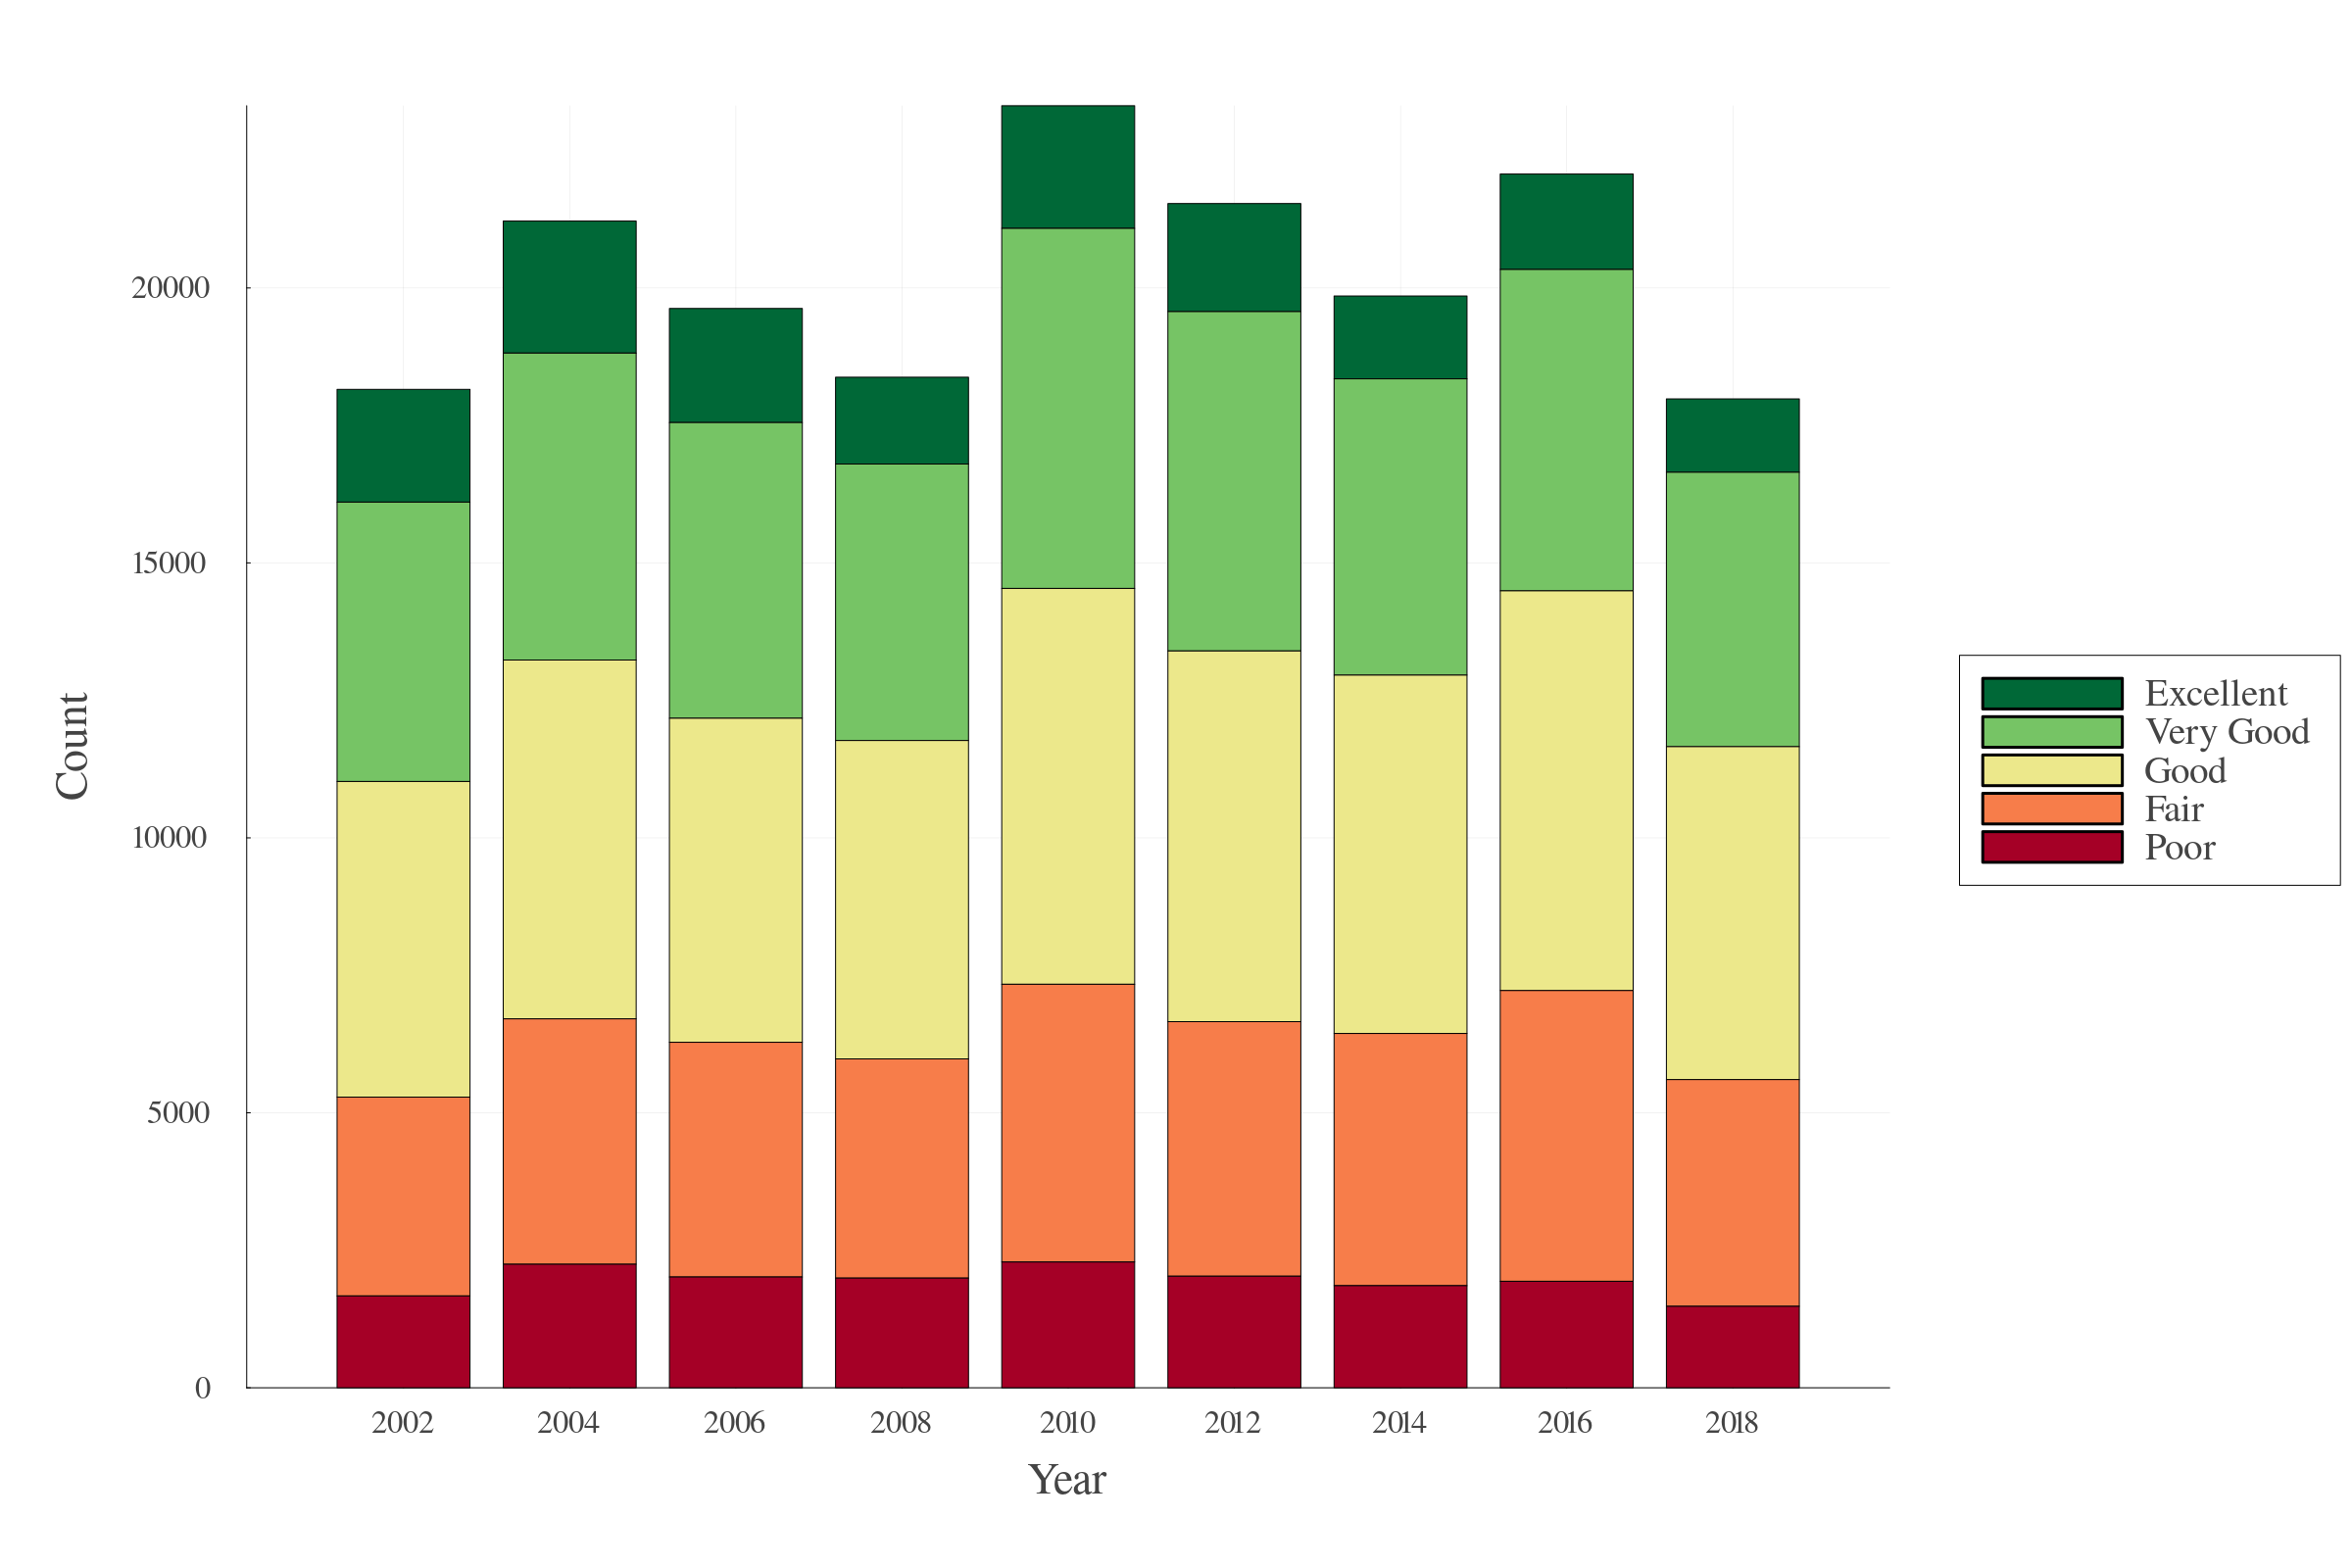
\includegraphics[width=\textwidth]{/Users/paulogcd/Documents/Master_Thesis/working_elements/Draft/output/histogram_1.png}
    \caption{Health Status distribution per Year, from the HRS data.}
\end{figure}

\subsubsection{Climate Data}

Temperature data are drawn from the Berkeley Earth project’s \textit{Land Monthly Average Temperature} dataset, which reports monthly global land surface temperature anomalies through time.
Anomalies are measured relative to the 1951–1980 baseline, with 95\% confidence bounds provided for each month.
Figure 2 shows the upward trend in global average land temperature over time.

The analysis uses global average annual temperature as the climatic variable.
This measure offers a tractable and transparent proxy, avoiding the complexity of regional variation while remaining informative.

Four temperature trajectories are considered for simulation.
The \textit{historical path} rises from 0 to 1.5°C between the mid-20th and mid-21st century. Three additional scenarios, drawn from IPCC projections for 2000–2100 and starting at 0.5°C, reflect broader possibilities: a \textit{pessimistic path} reaching 4°C, an \textit{intermediate path} reaching 3°C, and an \textit{optimistic path} stabilizing at 2°C.
These benchmark paths allow for structured comparisons of long-run effects on health and income.

\begin{figure}[H]
    \centering
    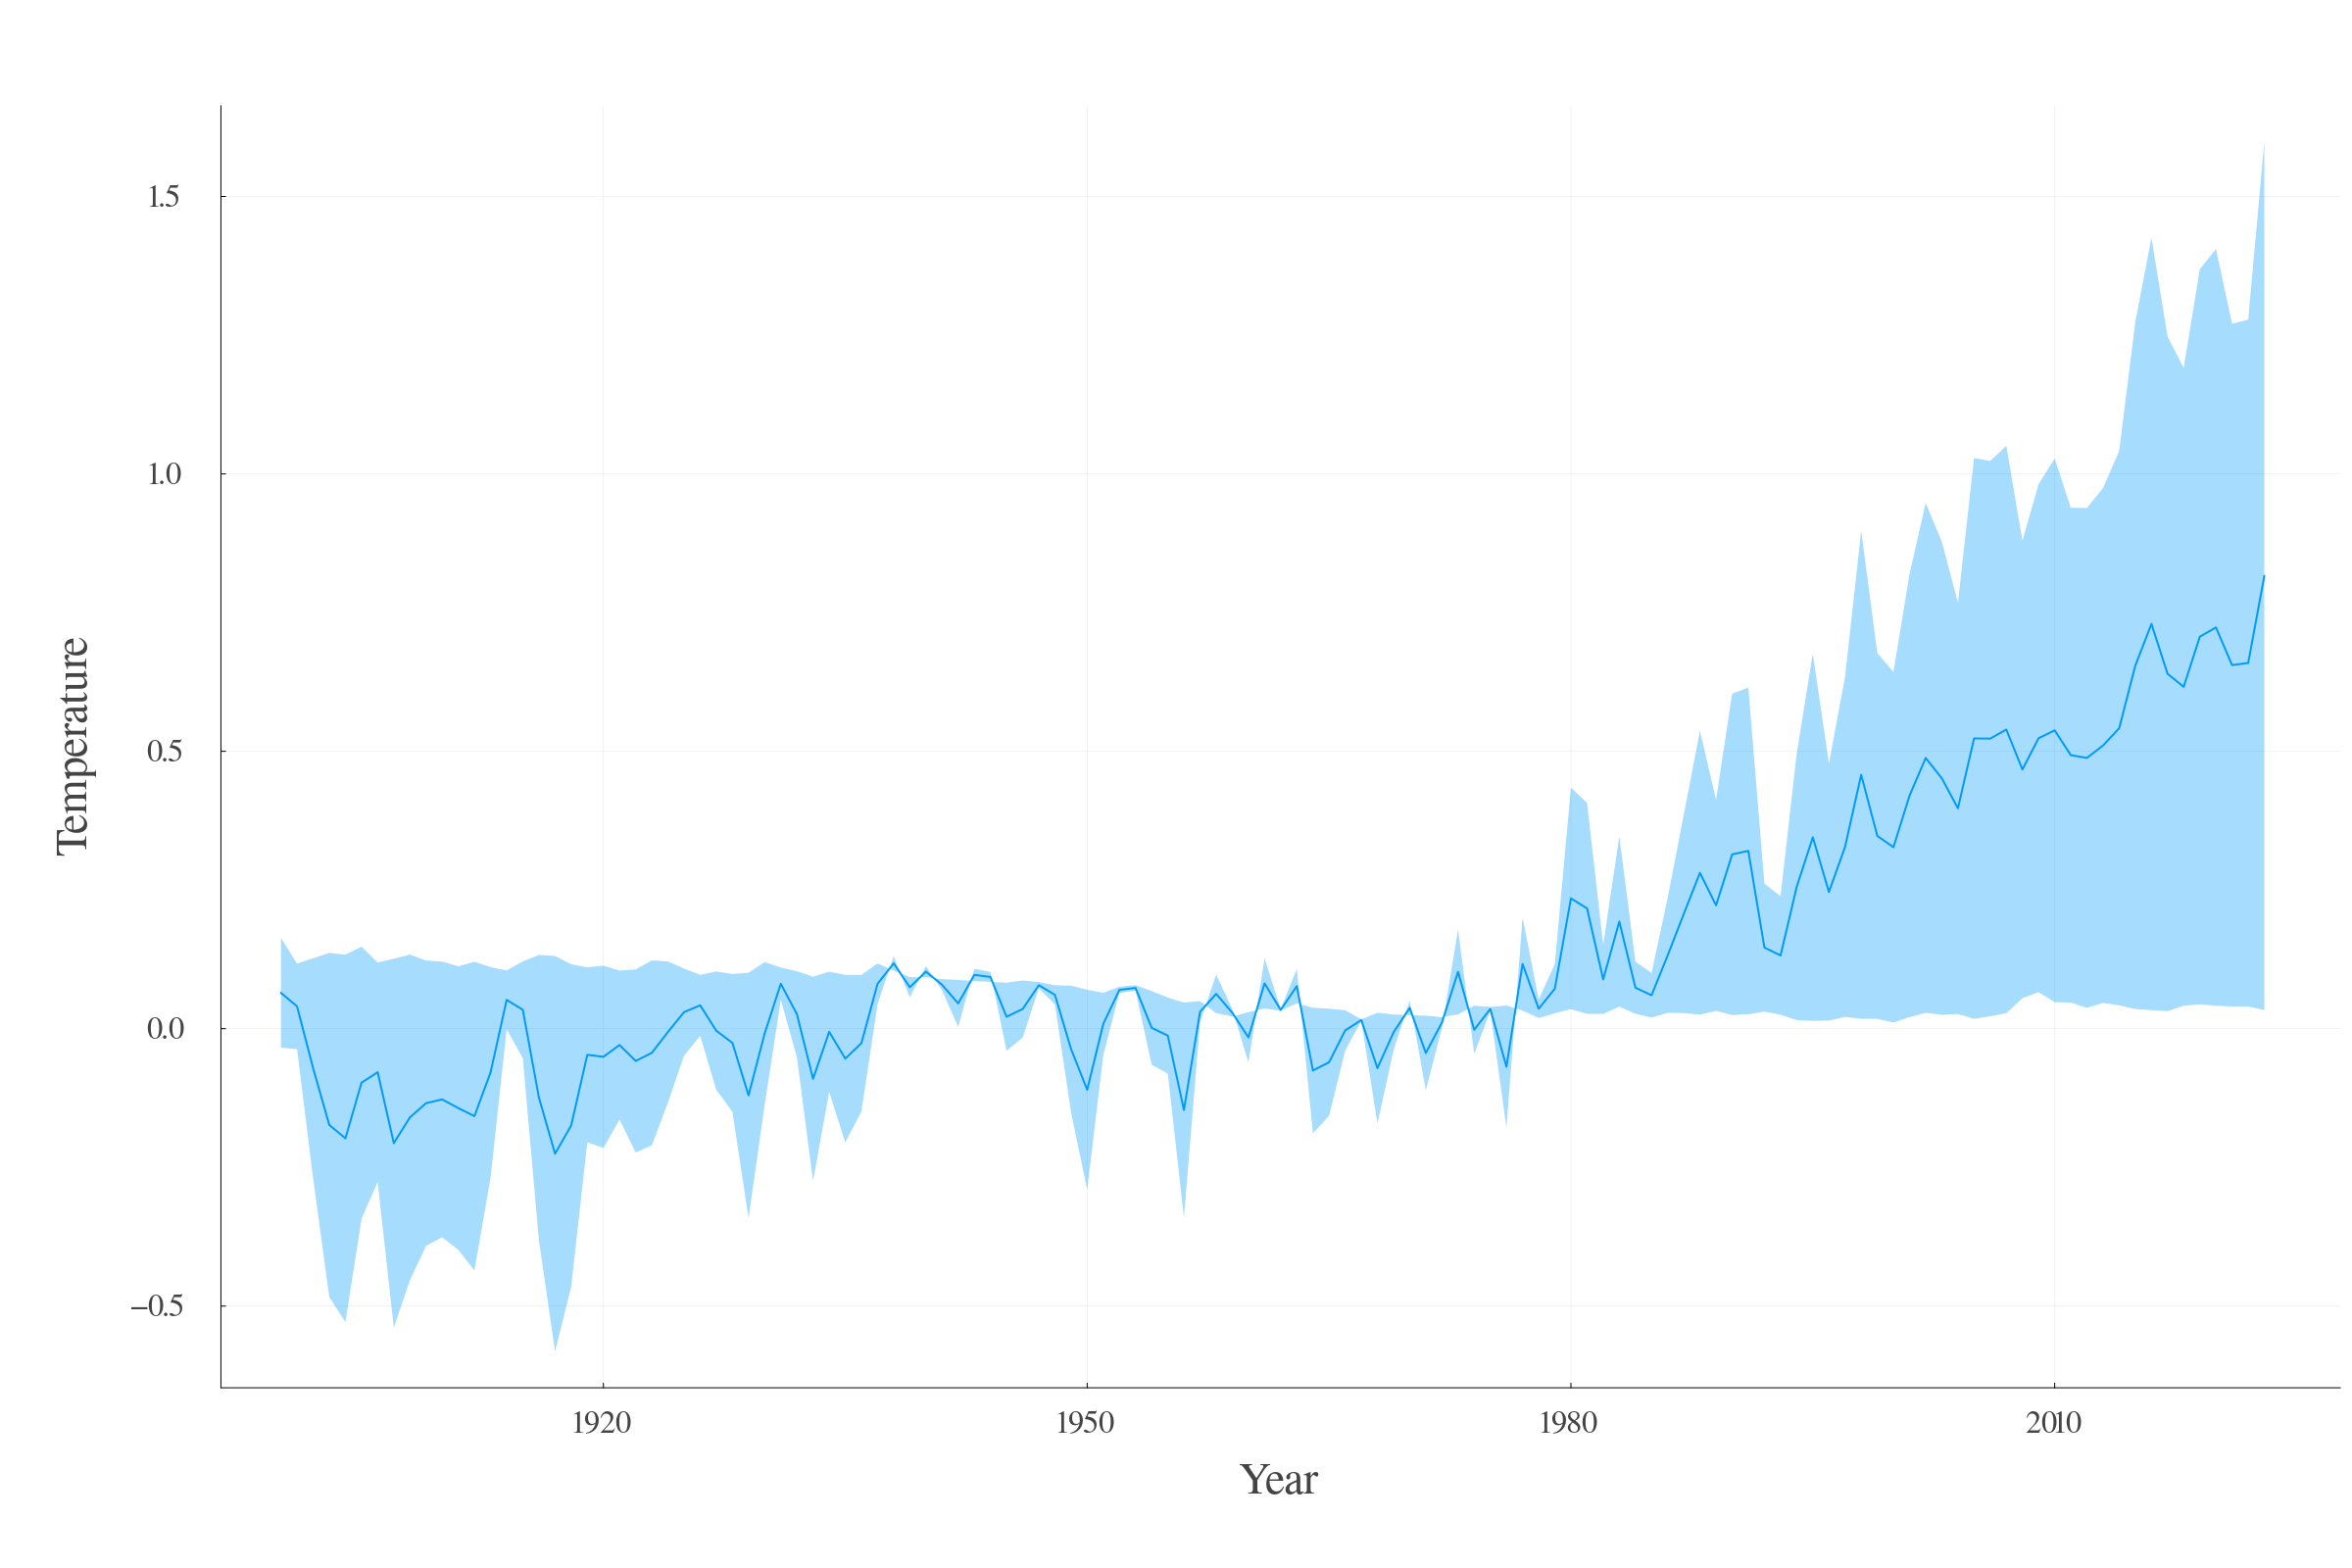
\includegraphics[width=\textwidth]{/Users/paulogcd/Documents/Master_Thesis/working_elements/Draft/output/figure_1.png}
    \caption{Evolution of Global Average Annual Temperature (1900–2022)}
    \caption*{\small The dark blue line plots the global average temperature anomaly relative to the 1951–1980 baseline.
    The light blue shaded area shows the 95\% confidence interval around each year’s estimate, as provided by the Berkeley Earth dataset.}
\end{figure}

\subsubsection{Economic Data}

Finally, economic data from the Federal Reserve Bank of St. Louis (FRED) are used for two purposes. 
Annual U.S. Gross Domestic Product (GDP) figures are employed in preliminary estimation exercises, 
while the long-run average interest rate is used to calibrate the discount factor in the economic model.

\section{Estimation of Health and Survival Dynamics}

This section presents the empirical framework used to estimate
the relationships between temperature,
individual health trajectories, and survival probabilities.
Using microdata from the Health and Retirement Study (HRS),
we focus on modeling health transitions and mortality risk
as functions of recent health status, temperature exposure, and age.

We begin by modeling health dynamics through an ordered response approach that
leverages the five-category self-reported health variable.
We then estimate survival probabilities using a binary outcome model,
again accounting for health and temperature effects.
To address concerns of omitted variable bias and potential collinearity, 
we introduce a Health Proxy, which allows for a tractable way to represent how
temperature might affect transitions via acute health risks. 

The resulting estimates capture a reduced-form
effect of climate variation on health and survival,
through a group of health risk,
and serve as key inputs for the economic
model introduced in the next section.

\subsection{Health Transition}

The Health and Retirement Study (HRS) provides detailed longitudinal data on individuals’ self-reported health, captured across five ordered categories.
To preserve the richness of this variable, it is not recoded into a binary indicator (e.g., “Good” vs. “Bad”) but retained in its full ordinal form, with $H \in \{1,\dots,5\}$ representing states from “Excellent” to “Poor” health.

Given the ordered and discrete nature of the outcome, health transitions are modeled using ordered response models. 
Specifically, the ordered logit, due to its tractability and widespread use in the literature \cite{Wooldridge_2010}.

For computational and identification reasons, we restrict the information set determining current health status to the most recent lag and contemporaneous temperature. That is, rather than modeling the full dependence $f_h(\mathcal{H}_{t-1}, \mathcal{W}_{t})$, we simplify the transition function to:
\[
f_{h}(H_{t-1}, T_{t}),
\]
where $T_t$ is the average annual temperature at time $t$.

Since health status takes values in a finite, ordered set, $f_h$ defines a categorical distribution (sometimes referred to as a generalized Bernoulli), and can be expressed as a transition function indexed by previous health status:
\[
f_{h}(H_{t-1} = j, T_{t}) = f_{h,j}(T_{t}), \quad \forall j \in \{1,\dots,5\}.
\]

To estimate these transition probabilities, one could consider a direct ordered logistic regression with $H_t$ as the dependent variable, and age, temperature, and other controls as covariates. However, this naive approach faces two major challenges. First, omitted variable bias: many unobserved factors, such as access to care or behavioral choices, can affect both health and survival. Second, collinearity: economic controls (such as GDP or health expenditures) are often strongly correlated with temperature trends, making it difficult to isolate causal effects.

Moreover, interaction effects between covariates are likely important.
For example, the impact of a given health state on future transitions may differ substantially by age: 
“Fair” health at age 30 has different implications than at age 80.

To address these concerns, we introduce a two-staged-regression inspired strategy.

We define a composite health shock measure, the \textit{Health Proxy} ($HP_{i,t}$), capturing the burden of recent temperature-sensitive health incidents.
This proxy is constructed as the sum of binary indicators for the presence of the following four health conditions:
\textit{High blood pressure},
\textit{Lung disease},
\textit{Heart condition},
\textit{Stroke}.
Formally:
\[
HP_{i,t} = \text{HighBP}_{i,t} + \text{Lung}_{i,t} + \text{Heart}_{i,t} + \text{Stroke}_{i,t}
\]

We first estimate a linear model for $HP_{i,t}$ as a function of age and temperature:
\[
\widehat{HP}_{i,t}^{I} = \widehat{\beta_0} + \widehat{\beta_A} \cdot \text{Age}_{i,t} + \widehat{\beta_T} \cdot T_t + \widehat{\beta_{A \times T}} \cdot (\text{Age}_{i,t} \times T_t)
\]

This first-stage regression provides a filtered proxy for temperature-induced health risks, which is then used in a second regression to estimate health transition probabilities. Specifically, we regress the probability of transitioning to a new health state on previous health status and the predicted health proxy $\widehat{HP}_{i,t}^{I}$, thus controlling for age and filtering out temperature's indirect effects via acute health events.
This two-step strategy allows us to better identify the effect of 
temperature on acute health state dynamics 
while mitigating omitted variable bias and accounting for age interactions.
\\

The first-stage regression results, presented in Table 1, provide empirical support for the construction of the Health Proxy as a function of age, temperature, and their interaction.
As expected, age is a strong and significant predictor of acute health conditions, with each additional year associated with a 0.02 increase in the composite health burden measure ($p < 0.001$).
The standalone effect of temperature is negative but statistically insignificant, suggesting that average annual temperature alone does not systematically explain acute health conditions in this sample.
However, the interaction term between age and temperature is positive and statistically significant at the 1\% level.
This indicates that the effect of temperature on health burden intensifies with age—a key channel motivating the use of $\widehat{HP}_{i,t}^I$ as a mediator in the second stage.
While the model explains only a modest portion of the variance in health conditions ($R^2 = 0.086$), this is expected given the many unobserved factors—such as genetic predisposition, lifestyle, or access to care—that drive acute health events. However, our primary goal is not to fully explain health shocks, but rather to isolate the marginal effects of temperature and age. In that respect, the significant interaction between age and temperature supports the interpretation of the Health Proxy as a temperature-sensitive health shock, particularly among older individuals.

\begin{table}[H]
    \begin{center}
        \begin{tabular}{lr}
            \toprule
                                    & \multicolumn{1}{c}{HP} \\ 
            \midrule
            (Intercept)              &              -0.487*** \\ 
                                    &                (0.068) \\ 
            Age                      &               0.020*** \\ 
                                    &                (0.001) \\ 
            Temperature              &                 -0.032 \\ 
                                    &                (0.123) \\ 
            Age $\times$ Temperature &                0.005** \\ 
                                    &                (0.002) \\ 
            \midrule
            $N$                      &                182,947 \\ 
            $R^2$                    &                  0.086 \\ 
            \bottomrule
        \end{tabular}
        \caption{Regression of Health Proxy on Age, Temperature, and their interaction.}
    \end{center}
\end{table}


\paragraph{Estimated Health Transition Probabilities.}
The two following figures depict the estimated probabilities of transitioning across self-reported health states as a function of age, conditional on the current health status.
The five health categories considered are \textit{Excellent}, \textit{Very Good}, \textit{Good}, \textit{Fair}, and \textit{Poor}.
These transition probabilities provide a dynamic picture of health deterioration (or improvement) over the life cycle.
For clarity purposes, temperature was not included in these graphics to avoid 3D plotting.
\footnote{Further graphical representations of transition probabilities are available in the Appendix.}
\\

From excellent health, the probability of
remaining in this health state declines steadily with age, while the proba
bility of transitioning to Very Good health increases. Transitions to lower
health states (Good, Fair, Poor) remain unlikely but grow slowly over
time. This indicates that while aging naturally erodes top health status,
the decline is gradual and dominated by moves to slightly lower but still
positive states.

\begin{figure}[H]\label{fig:health_transition_1}
    \begin{center}
        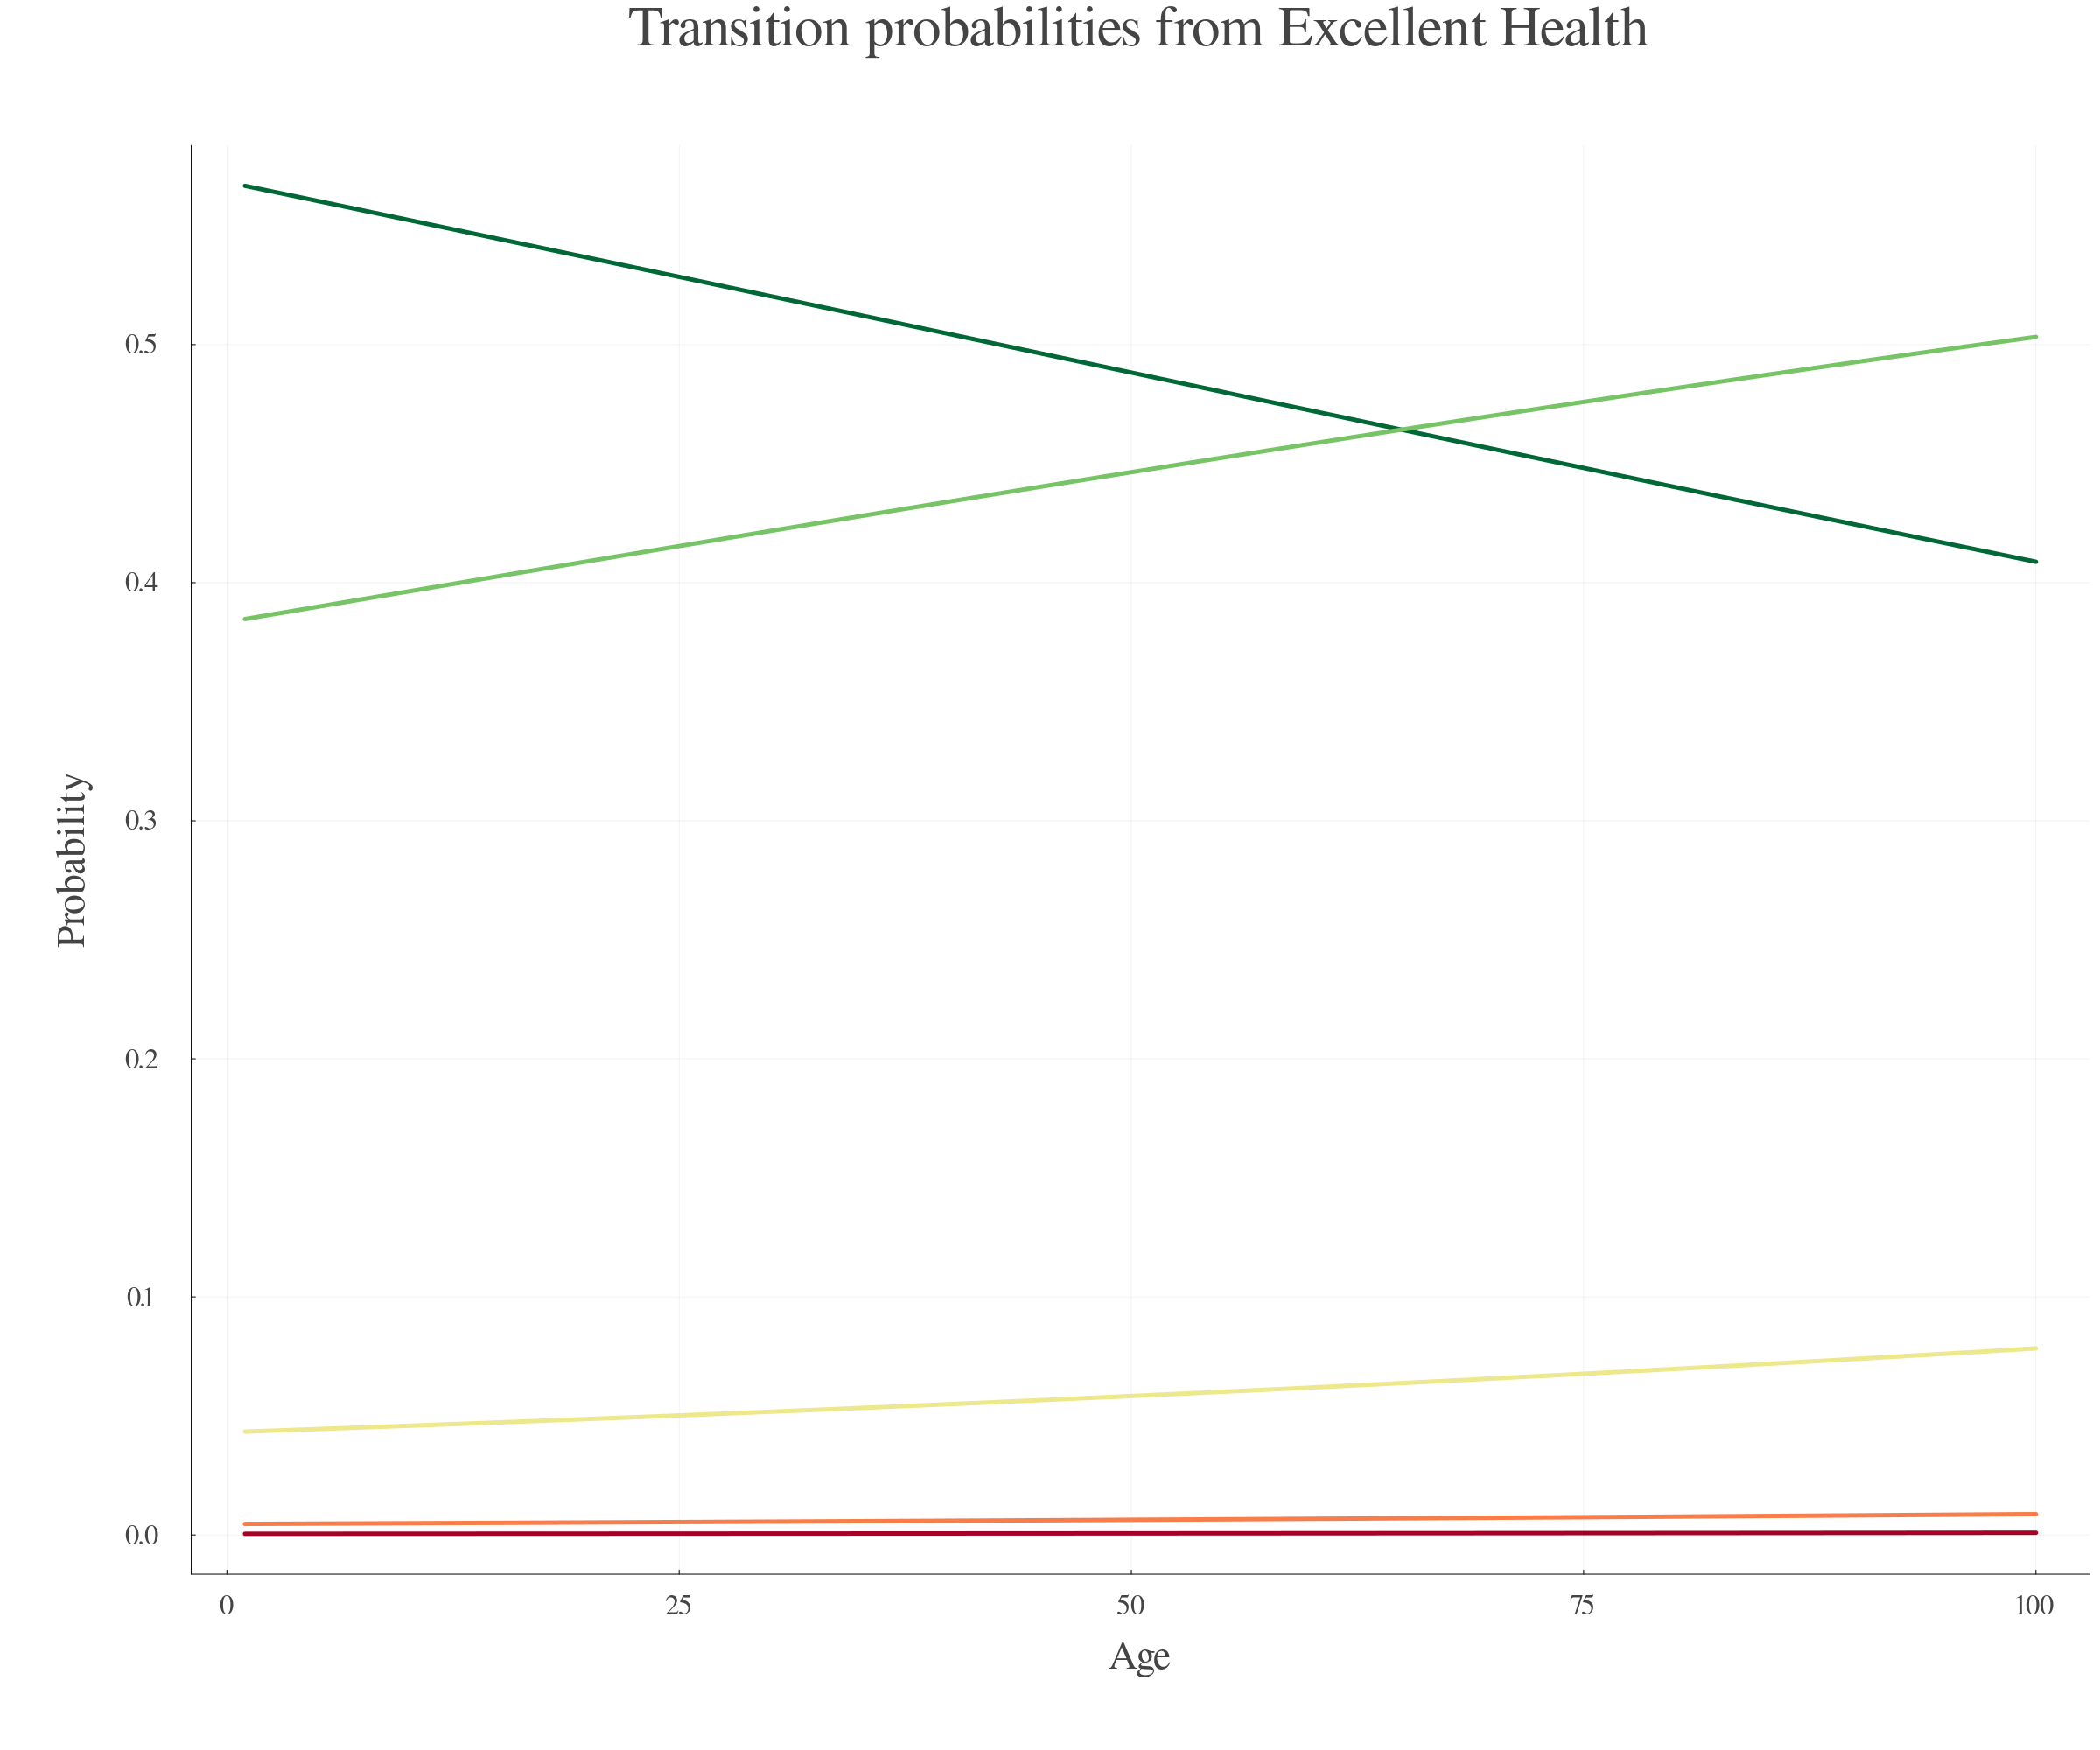
\includegraphics[width=\linewidth]{output/health_transition_1.png}
        \caption{Transition probabilities from Excellent Health}    
    \end{center}
\end{figure}

In the opposite case, the probability of remaining in \textit{Poor} health increases markedly with age, surpassing 60\% by age 100.
Improvements to better health categories become virtually negligible with age, suggesting that \textit{Poor} health is largely an absorbing state for older individuals.
\begin{figure}\label{fig:health_transition_5}
    \begin{center}
        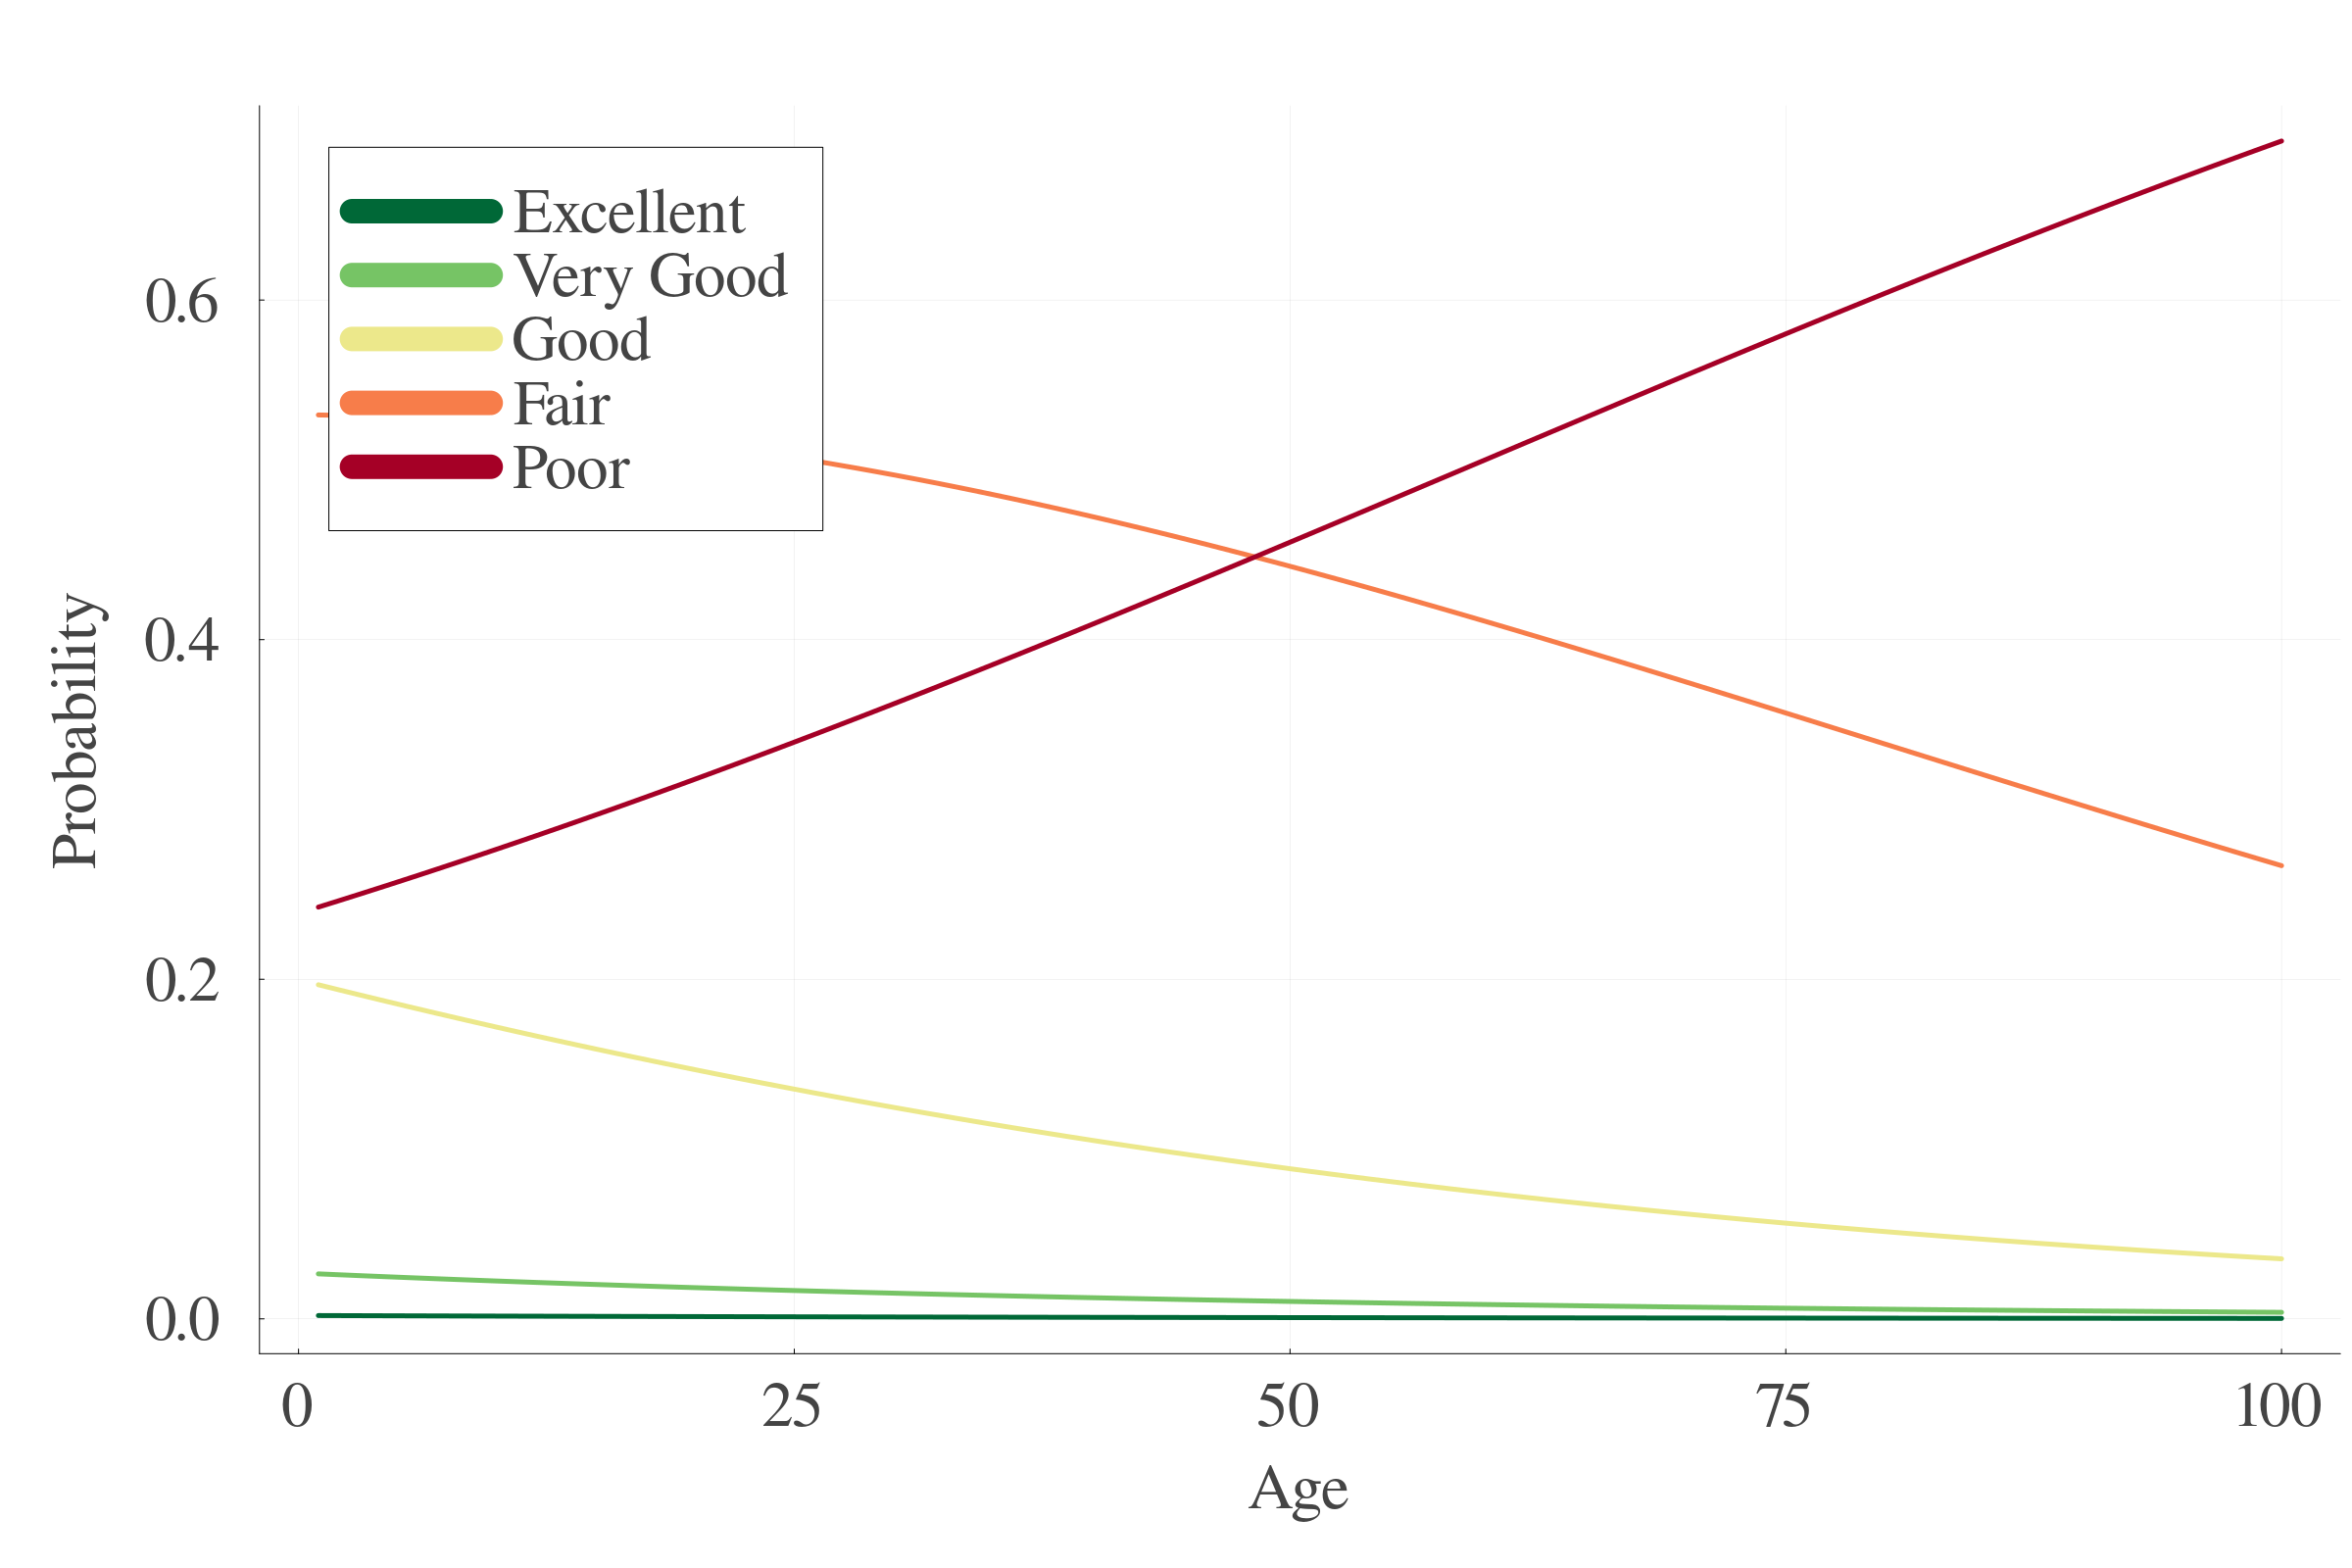
\includegraphics[width=\linewidth]{output/health_transition_5.png}
        \caption{Transition probabilities from Poor Health}   
    \end{center} 
\end{figure}


These estimated transition probabilities highlight the persistent and age-dependent nature of health status. They support the modeling assumption of a health process that becomes increasingly inertial with age, and they reflect the empirical reality that upward health mobility becomes rarer in older populations. This framework is essential for evaluating how external shocks—such as temperature-driven health shocks—interact with baseline health dynamics across the life cycle.
Based on these estimates, 
it is alread possible to perform 
simulations of different groups of individuals with specific temperature trajectories. 
\footnote{A specific illustration is available in the Appendix.}

\subsection{Living Status}
The binary nature of the living status variable allows for a straightforward application of logistic regression.

To estimate the survival probability \( p_t(\mathcal{H}_t, \mathcal{W}_t) \), a naive regression approach would encounter similar issues to those previously discussed.
For instance, estimating a regression using only GDP as a covariate leads to a negative coefficient not only on temperature but also on GDP.
This counterintuitive result reflects a recent trend in the United States, where GDP has continued to grow substantially, while life expectancy has remained stagnant or slightly declined.
As such, preliminary results showed the necessity of adapting the regression specification, as it is done by the Health Proxy $HP_{i,t}$, as explained above.

Using the logistic function \( \Lambda(\cdot) \), we estimate the individual survival probability \( p_{i,t} \) at time \( t \) via the following specification, which incorporates the previously estimated health proxy \( \widehat{HP}_{i,t}^{I} \):

\begin{equation}
    \widehat{p_{i,t}} = \Lambda \left( \widehat{\beta_0} +
    \widehat{\beta_{H}} \cdot Health_{i,t} +
    \widehat{\beta_{HP}} \cdot \widehat{HP}_{i,t}^{I} \right)
\end{equation}

By combining the health transition probabilities with these survival probability estimates, we can simulate and visualize the demographic dynamics of a population over time.
This is illustrated in the next figure, which shows the annual survival probability as a function of both age and health status, based on an initial population of \( N_0 = 10{,}000 \).

\begin{figure}[H]
    \centering
    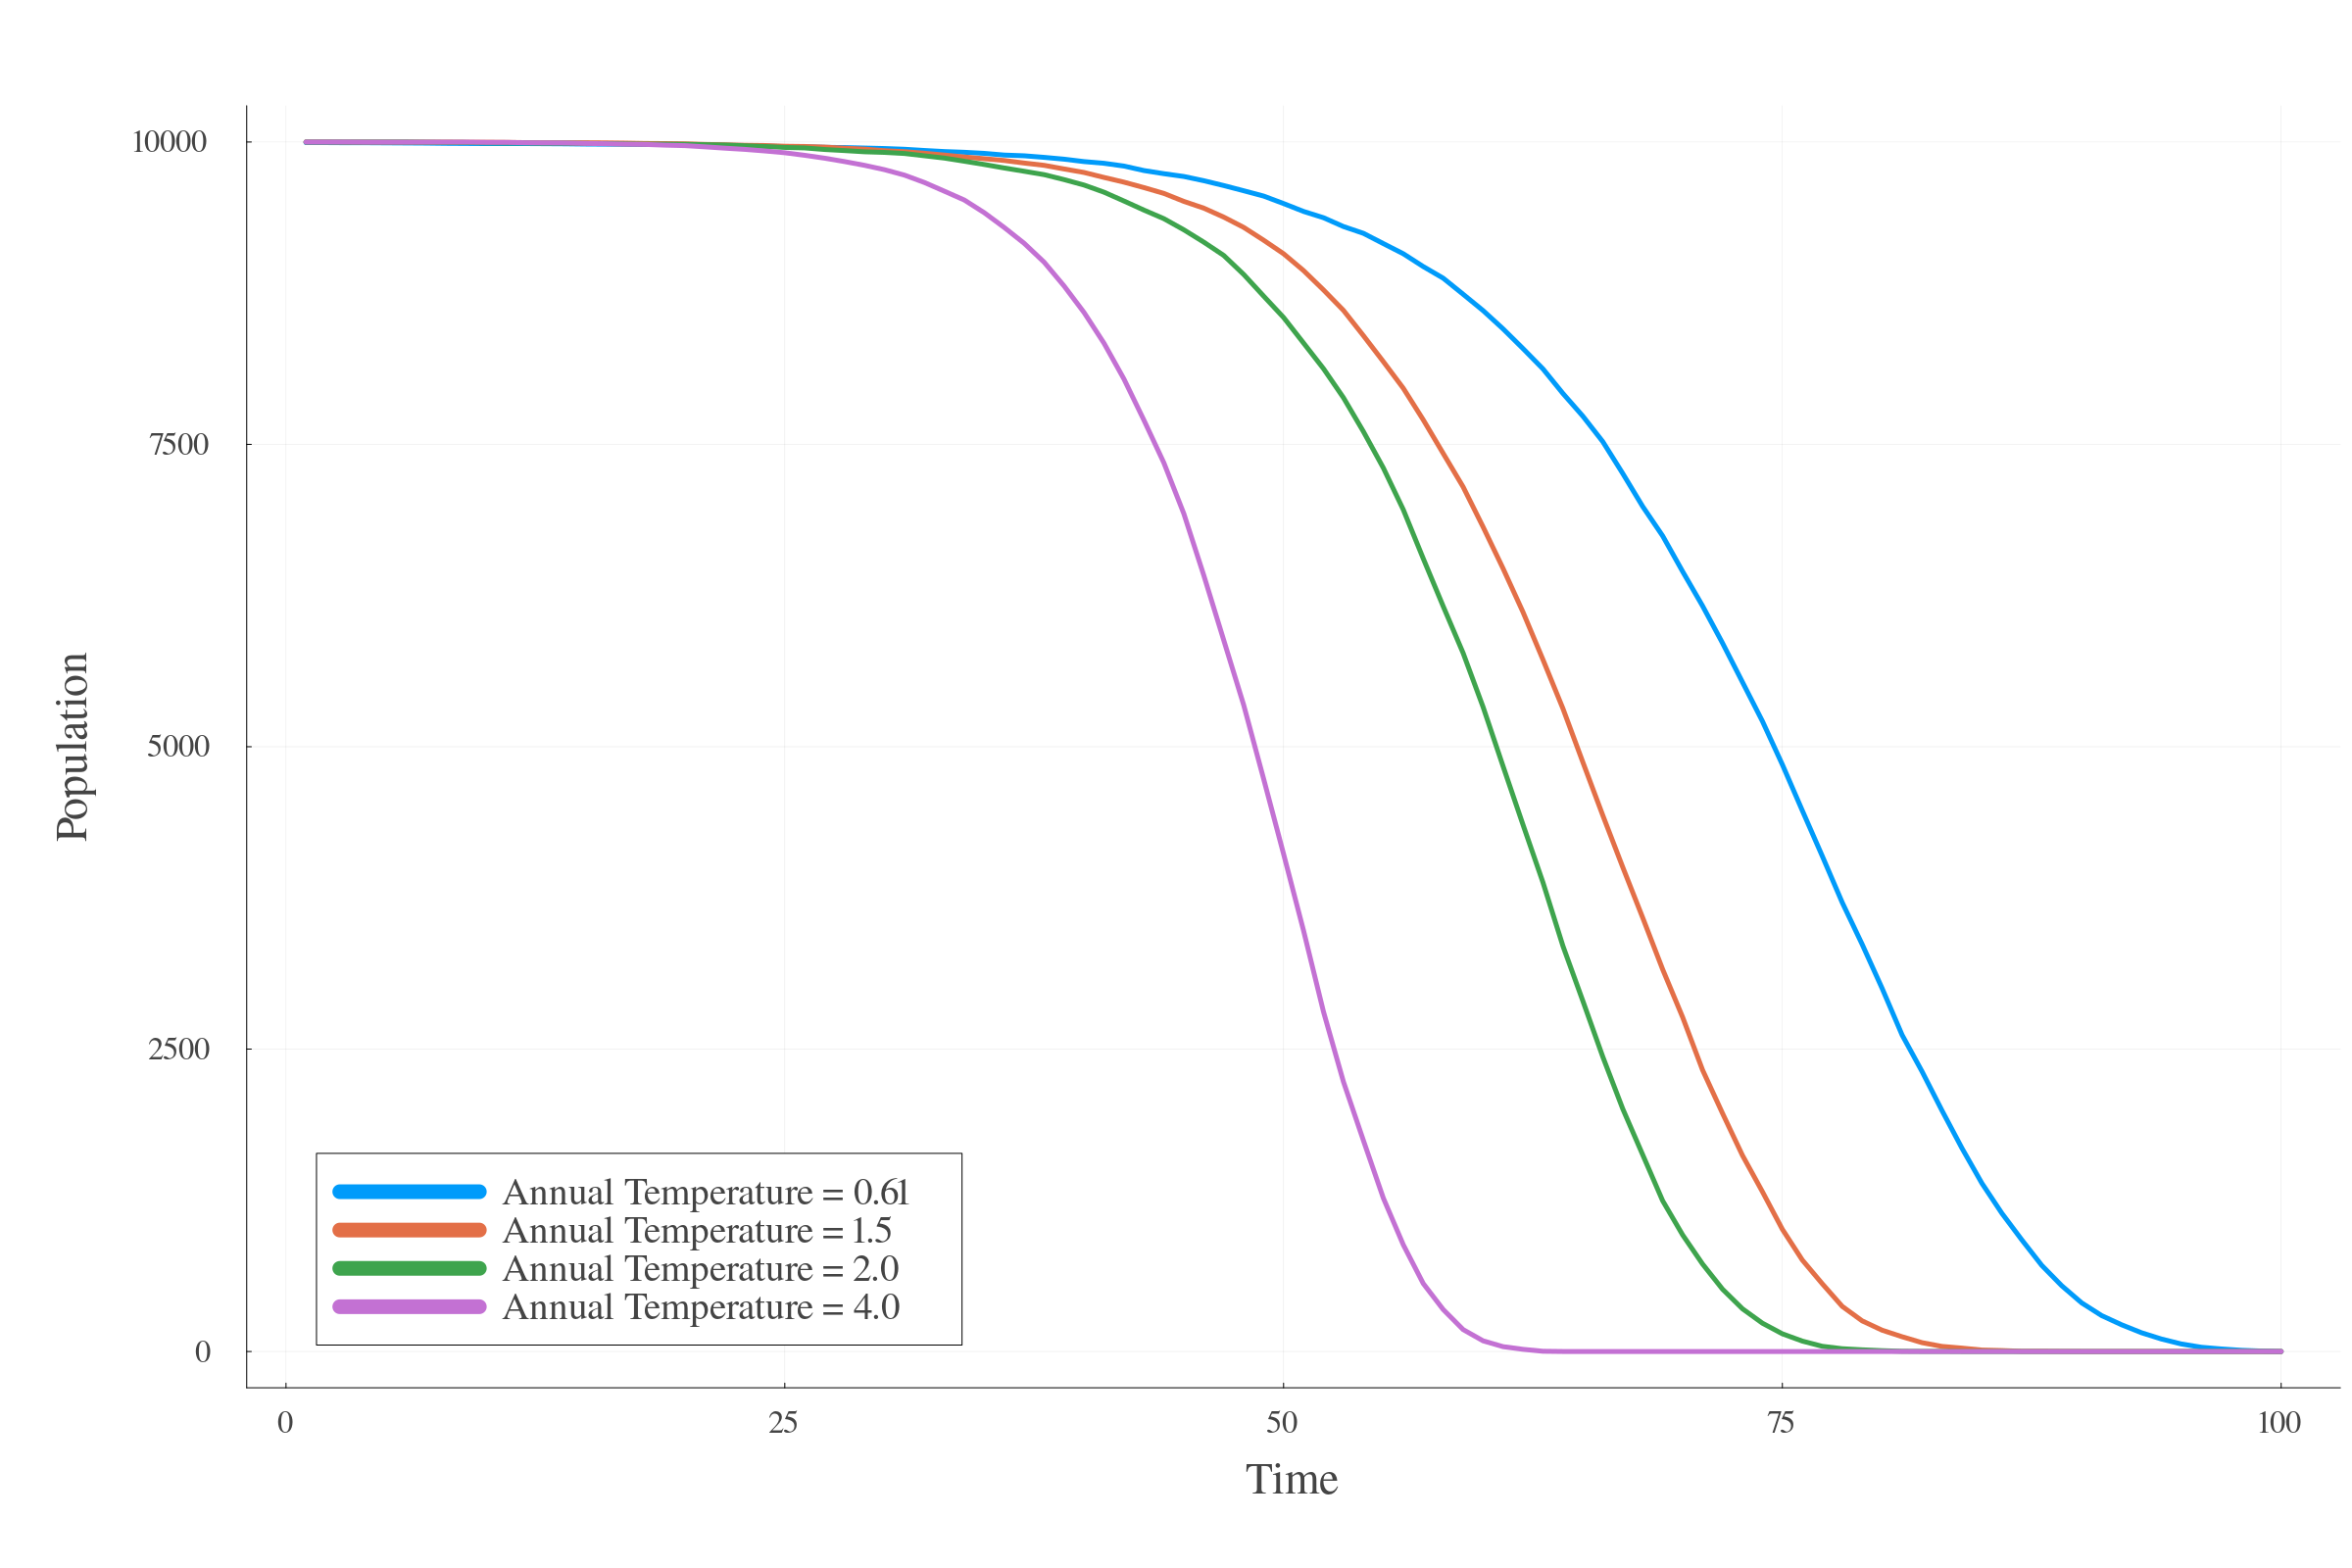
\includegraphics[width=\textwidth]{/Users/paulogcd/Documents/Master_Thesis/working_elements/Draft/output/figure_3.png}
    \caption{Annual probability of survival as a function of age and health status, obtained with \( N_0 = 10{,}000 \).}
    \label{survival_probability}
\end{figure}

Higher temperatures can exacerbate acute health conditions, particularly among vulnerable populations such as the elderly or those with pre-existing health issues.
For instance, extreme heat has been linked to cardiovascular stress, respiratory complications, and increased incidence of heat-related illnesses.
These acute conditions can accelerate transitions from better to worse health states and elevate mortality risk.
Furthermore, temperature interacts with age in a non-linear fashion. Older individuals generally have reduced thermoregulatory capacity, making them more susceptible to heat stress.
As a result, even moderate increases in temperature can disproportionately affect their survival probabilities and hasten deterioration in health status.
Therefore, the negative coefficient on temperature is not merely a statistical artifact but reflects real physiological and epidemiological mechanisms.
This compound influence (affecting both the likelihood of transitioning to a worse health state and the immediate probability of survival) drives the overall negative relationship between temperature and life expectancy observed in our model.

These estimates are now going to be used in 
the economic model.

\section{Model}

This section is dedicated to the formal description of 
the model, as well as its analytical analysis.
First, its main mechanisms will be explained, and then, the 
nonexistence of analytical solution in most cases will be shown.

\subsection{Baseline specification }

The agents maximize: 

$$ \max_{\{c_{t},l_{t},s_{t+1}\}_{t=1}^{100}}{\mathbb{E}\left[\sum_{t=1}^{100} \beta^{t}\cdot u(c_t,l_t)\right]}$$

Their utility function is: 

$$u(c_{t},l_{t}) = \frac{c_{t}^{1-\rho}}{1-\rho}-\xi_{t}\cdot \frac{l_{t}^{1+\varphi}}{1+\varphi}$$

With : 

-  $c_{t}$  the consumption

-  $l_{t}$  the quantity of labor supply provided by the agent

-  $h_{t}$  the health status

-  $w_{t}$  the weather variable, which is here temperature

-  $\xi_{t}$ the labor disutility coefficient

- $\rho$ the risk aversion coefficient

- $\varphi$ the Frisch elasticity of Labor supply.
\\

The agent is subject to the following budget constraint:

$$c_{t} + s_{t+1} \leq l_{t}\cdot z_{t} + s_{t}\cdot(1+r_{t})$$

With: 

-  $c_t$ the consumption at period $t$

-  $s_{t+1}$ the savings for period $t+1$

-  $l_t$ the labor supply provided by the agent at period $t$

-  $z_t$ the productivity at time $t$

-  $s_{t}$ the savings available at the beginning of period $t$

-  $r_{t}$ the interest rate at period $t$

Also, agents are subject to the following borrowing constraint, defined as: 

$$s_{t+1}\geq \underline{s}, \forall t \in [\![1,T]\!]$$


We can note the First Order Conditions, such that: 

\begin{equation}
    c^{-\rho}_{t}\cdot z_{t} = \xi_{t}\cdot l_{t}^{\varphi} \iff
        \begin{cases}
        & c_t = \left[\frac{\xi_{t}\cdot l_{t}^{\varphi}}{z_{t}}\right]^{-\frac{1}{\rho}}\\ 
        & l_{t} = \left[\frac{c_{t}^{-\rho}z_{t}\cdot}{\xi_{t}}\right]^{\frac{1}{\varphi}}
    \end{cases}
\end{equation}
And 
\begin{equation}
    c^{-\rho}_{t} = \beta \cdot \mathbb{E}\left[c^{-\rho}_{t+1}\cdot (1+r_{t+1})\right] + \gamma_{t}
\end{equation}

The first corresponds to the equalization of marginal benefit and
cost of labor, and the second corresponds to the Euler equation.

The first equilibrium condition implies an within decision,
driven by the labor disutility coefficient $\xi$ and the productivity $z$.
There is a unique mapping between consumption and labor at any period, to 
equalize the benefits and the costs of labor.

The second equilibrium condition implies an intertemporal decision.
The marginal utility of consumption at one period must be equal to the 
expected marginal utility of consumption next period, discounted by 
the discounting factor $\beta$ and the interest rate next period $(1+r_{t+1})$, 
plus the marginal benefit of violating the borrowing constraint at the current period. 

It is now important to describe what the Expectation operator $\mathbb{E}$ entails here. 
In a generic formulation, one could expect the uncertainty to affect the interest rate at the next period, 
which is the reason $(1+r_{t+1})$ is within the operator.

Another specification could exclude any uncertainty from 
the interest rate. 
The uncertainty could then come from the health and survival draw. 
If the uncertainty only comes from these two draws, the expectation operator can be formalized such as: 

$$\mathbb{E}\left[c_{t+1}\right] \equiv p_{t+1}(\mathcal{H}_{t},\mathcal{W}_{t}) \cdot c_{t+1}$$

\subsection{Analytical Solution nonexistence}

\textbf{Proposition}
This maximization program is impossible to solve analytically in most cases\footnote{The proof of this proposition is in the Appendix.}.
\\

If we consider the model altogether, it is impossible to describe 
analytically the optimal policy functions of the three choice variables.
While the entire proof is available in the appendix, a quick explanation
is possible here.
First, the objective functions is linear with the savings at next period $s_{t+1}$, 
making it disappear from the F.O.C.s.
This term requires therefore the labor and consumption policies to be solved, 
and then plugged into the budget constraint, to have a solution. 
However, if we try to solve the two other policy functions, 
we end up with transcendental equations of the form $a\cdot x^{\alpha} + b\cdot x + c = 0$, 
with $\alpha\notin \mathbb{N}$. 
These transcendental equations can be overcome with specific combinations 
of parameters, but these are however absurd in our context.
This nonexistence of analytical solution calls therefore for a numerical solving of the model.
The next section discusses the different methods used in order to do so.

\section{Numerical methods}

Several ways have been considered to solve this model numerically. 
This section is dedicated to the presentation of the different methods
used in order to do so. 
First, the auxiliary functions are presented. 
Second, the different main algorithms specifications and their performance are presented. 
Finally, the aggregation methods and different numerical results are discussed.

\subsection{Functions}

This subsection is dedicated to the description of the 
fundamental programmatic functions that were used to solve the model
numerically. 

\begin{itemize}
    \item \textbf{Budget clearing function: } 
    The budget clearing function computes the amount of non used income for a 
    set of state and choice variables. Since at optimal, the budget constraint is binding, 
    the underlying theoretical result indicates that the budget clearing function should be 
    zero. Given the imprecision of numerical methods, the average budget clearing function was used 
    as a measure of the precision performance of each algorithm.

    It is equal to: 
    $$B(s_{t},l_{t},c_{t},s_{t+1})=l_{t} \cdot z_{t} + s_{t}\cdot(1+r_{t}) - s_{t+1} - c_{t}$$

    \item \textbf{Bellman function: }
    The Bellman function takes as an argument the value function next period, 
    and maximizes the current utility plus the discounted value function next period. 

    It is equal to: 
    $$V(s_{t}) = \max_{\{c_{t},l_{t},s_{t+1}\}\in \Gamma(s_{t})} \{u(c_{t},l_{t}) + \beta \cdot V(s_{t+1})\}$$
    With $\Gamma(s_{t})$ the feasibility set given by the state variable $s_{t}$.

    \item \textbf{Backwards function: }
    The backwards function iterates the Bellman function from the last period 
    to the first one. In the case of policy iteration, it iterates over the 
    policy function, and not the value function. It aggregates the optimal decisions 
    and returns a grid of optimal choices associated to each period and state variable value.

    For the pure numerical value function iteration, the backwards function is
    as following: 
    \begin{figure}[H]
    \begin{lstlisting}[basicstyle=\small]
for t from 100 to 1

    if t is equal to 100
        Bellman next period = Vector of zeros
    end

    for s in the possible set of s
        for c,l,s' in the feasible set of the current s value
            
            # We compute the budget clearing: 

            bc = budget_clearing(c,l,s') 

            # If it does not,
            # we set the value function to a very low number.
            
            if bc < 0

                V[c,l,s',s] = -Inf 
            
            # If it does, we compute the value function 
            # for this combination of choice variables.
            
            else if bc >= 0

                V[c,l,s',s] =
                    utility(c,l,s') +
                    beta * probability of survival *
                    Bellman next period[s']
            end
        end
        
        # We set the value function for s and t to
        # the maximum value found.
        
    end

# We set the value function at next period to current one
Bellman_next_period = Value_function[index_s,t]

end
\end{lstlisting}
\caption{Pseudo-code of the backward function.}
\end{figure}

\end{itemize}


\subsection{Algorithms}

This section details the different algorithms
built upon the above-mentioned fundamental functions.
Indeed, if one can think of the pure numerical value function iteration to solve 
the model, multiple approaches exist, that vary depending on the targeted tradeoff 
between precision performance and speed performance\footnote{For more information, the different steps of the algorithms and their source code are available online.
The steps and comments of the present work are available here: \url{https://www.paulogcd.com/Master_Thesis/},
and the documented replication package, coded in Julia, is available here: \url{https://www.paulogcd.com/Master_Thesis_Paulogcd_2025/}.}. 

\subsubsection{Pure numerical value function iteration}

The pure numerical value function iteration algorithm consists
in verifying all possible 
combination of choice variables for each level of state variable 
to determine what is the best possible response given a certain
amount of state variable.

Here, the algorithm goes through all the possible values of
$c$, $l$, and $s'$, without using any approximation obtained 
through the FOC mentioned above. 
This is quite computational-intensive, but 
has the advantage of not using analytical results, 
which can lead to approximation depending on the resolution of the 
ranges used.

\subsubsection{F.O.C. approximated value function iteration}

The FOC approximated value function iteration algorithms
make use of the two expression of consumption and labor supply 
derived from the FOC
seen in the previous section. 
They are faster by orders of magnitudes when compared to the pure numerical 
value function iteration algorithm,
but contain more errors, measured by the budget clearing function\footnote{Note that it is impossible to use the second FOC, i.e. the 
Euler equation, containing the 
Lagrangian multiplier $\gamma_{t}$. 
However, the numerical solving process 
allows for an estimation of $\gamma_{t}$.}.

\subsubsection{Interpolated algorithms}

The interpolated algorithms 
use interpolation techniques to approximate 
the value of the next period Bellman equation. 
This interpolation can be implemented in the pure numerical 
algorithm, and in the FOC-approximated ones. 

They allow for a smoother shape of policy function, 
and have graphical results that are more easily interpretable.
However, their speed
performance is slightly worse, 
and the effect of interpolation on precision
performance is ambiguous. 

\subsection{Performance}

\begin{figure}[H]
    \begin{tabular}{cccc}
    \toprule
    Algorithm & Error & Time (in seconds) & Memory (in Mb)\\
    \midrule
    \makecell{Pure Numerical Value \\ Function Iteration} & 0.0179 & 0.6604 & 1033.4409\\
    \\
    \makecell{FOC approximation 1 \\ (fixing labor supply)} & 0.042 & 0.2506 & 98.1834\\
    \\
    \makecell{FOC approximation 2 \\ (fixing consumption)} & 0.042 & 0.0188 & 55.6981\\
    \bottomrule
    \end{tabular}
    \caption{Algorithms and their performance.\\
    These results were obtained from reduced ranges, but scale exponentially.}
\end{figure}

\subsection{Policy Function Results}

This subsection is dedicated to the presentation of the policy function 
results from the numerical methods. 

The calibration was done following
the used in the found literature, 
and in order to make the numerical resolution possible.
The interest rate and discount factor were obtained after averaging
the past interest rate, from the FRED data mentioned previously.

\begin{table}[H]
\centering
\caption{Model Parameter Values}
\label{tab:parameters}
\begin{tabular}{lc}
\toprule
\textbf{Parameter} & \textbf{Value} \\
\midrule
Risk aversion coefficient ($\rho$) & 1.50 \\
Labor supply Frisch elasticity ($\varphi$) & 2.00 \\
Discount factor ($\beta$) & $\frac{1}{1+r} \approx 0.9825$ \\
Annual interest rate ($r$) &  $0.0178$ (1.78\%) \\
\bottomrule
\end{tabular}
\end{table}

\begin{figure}[H]
    \centering
    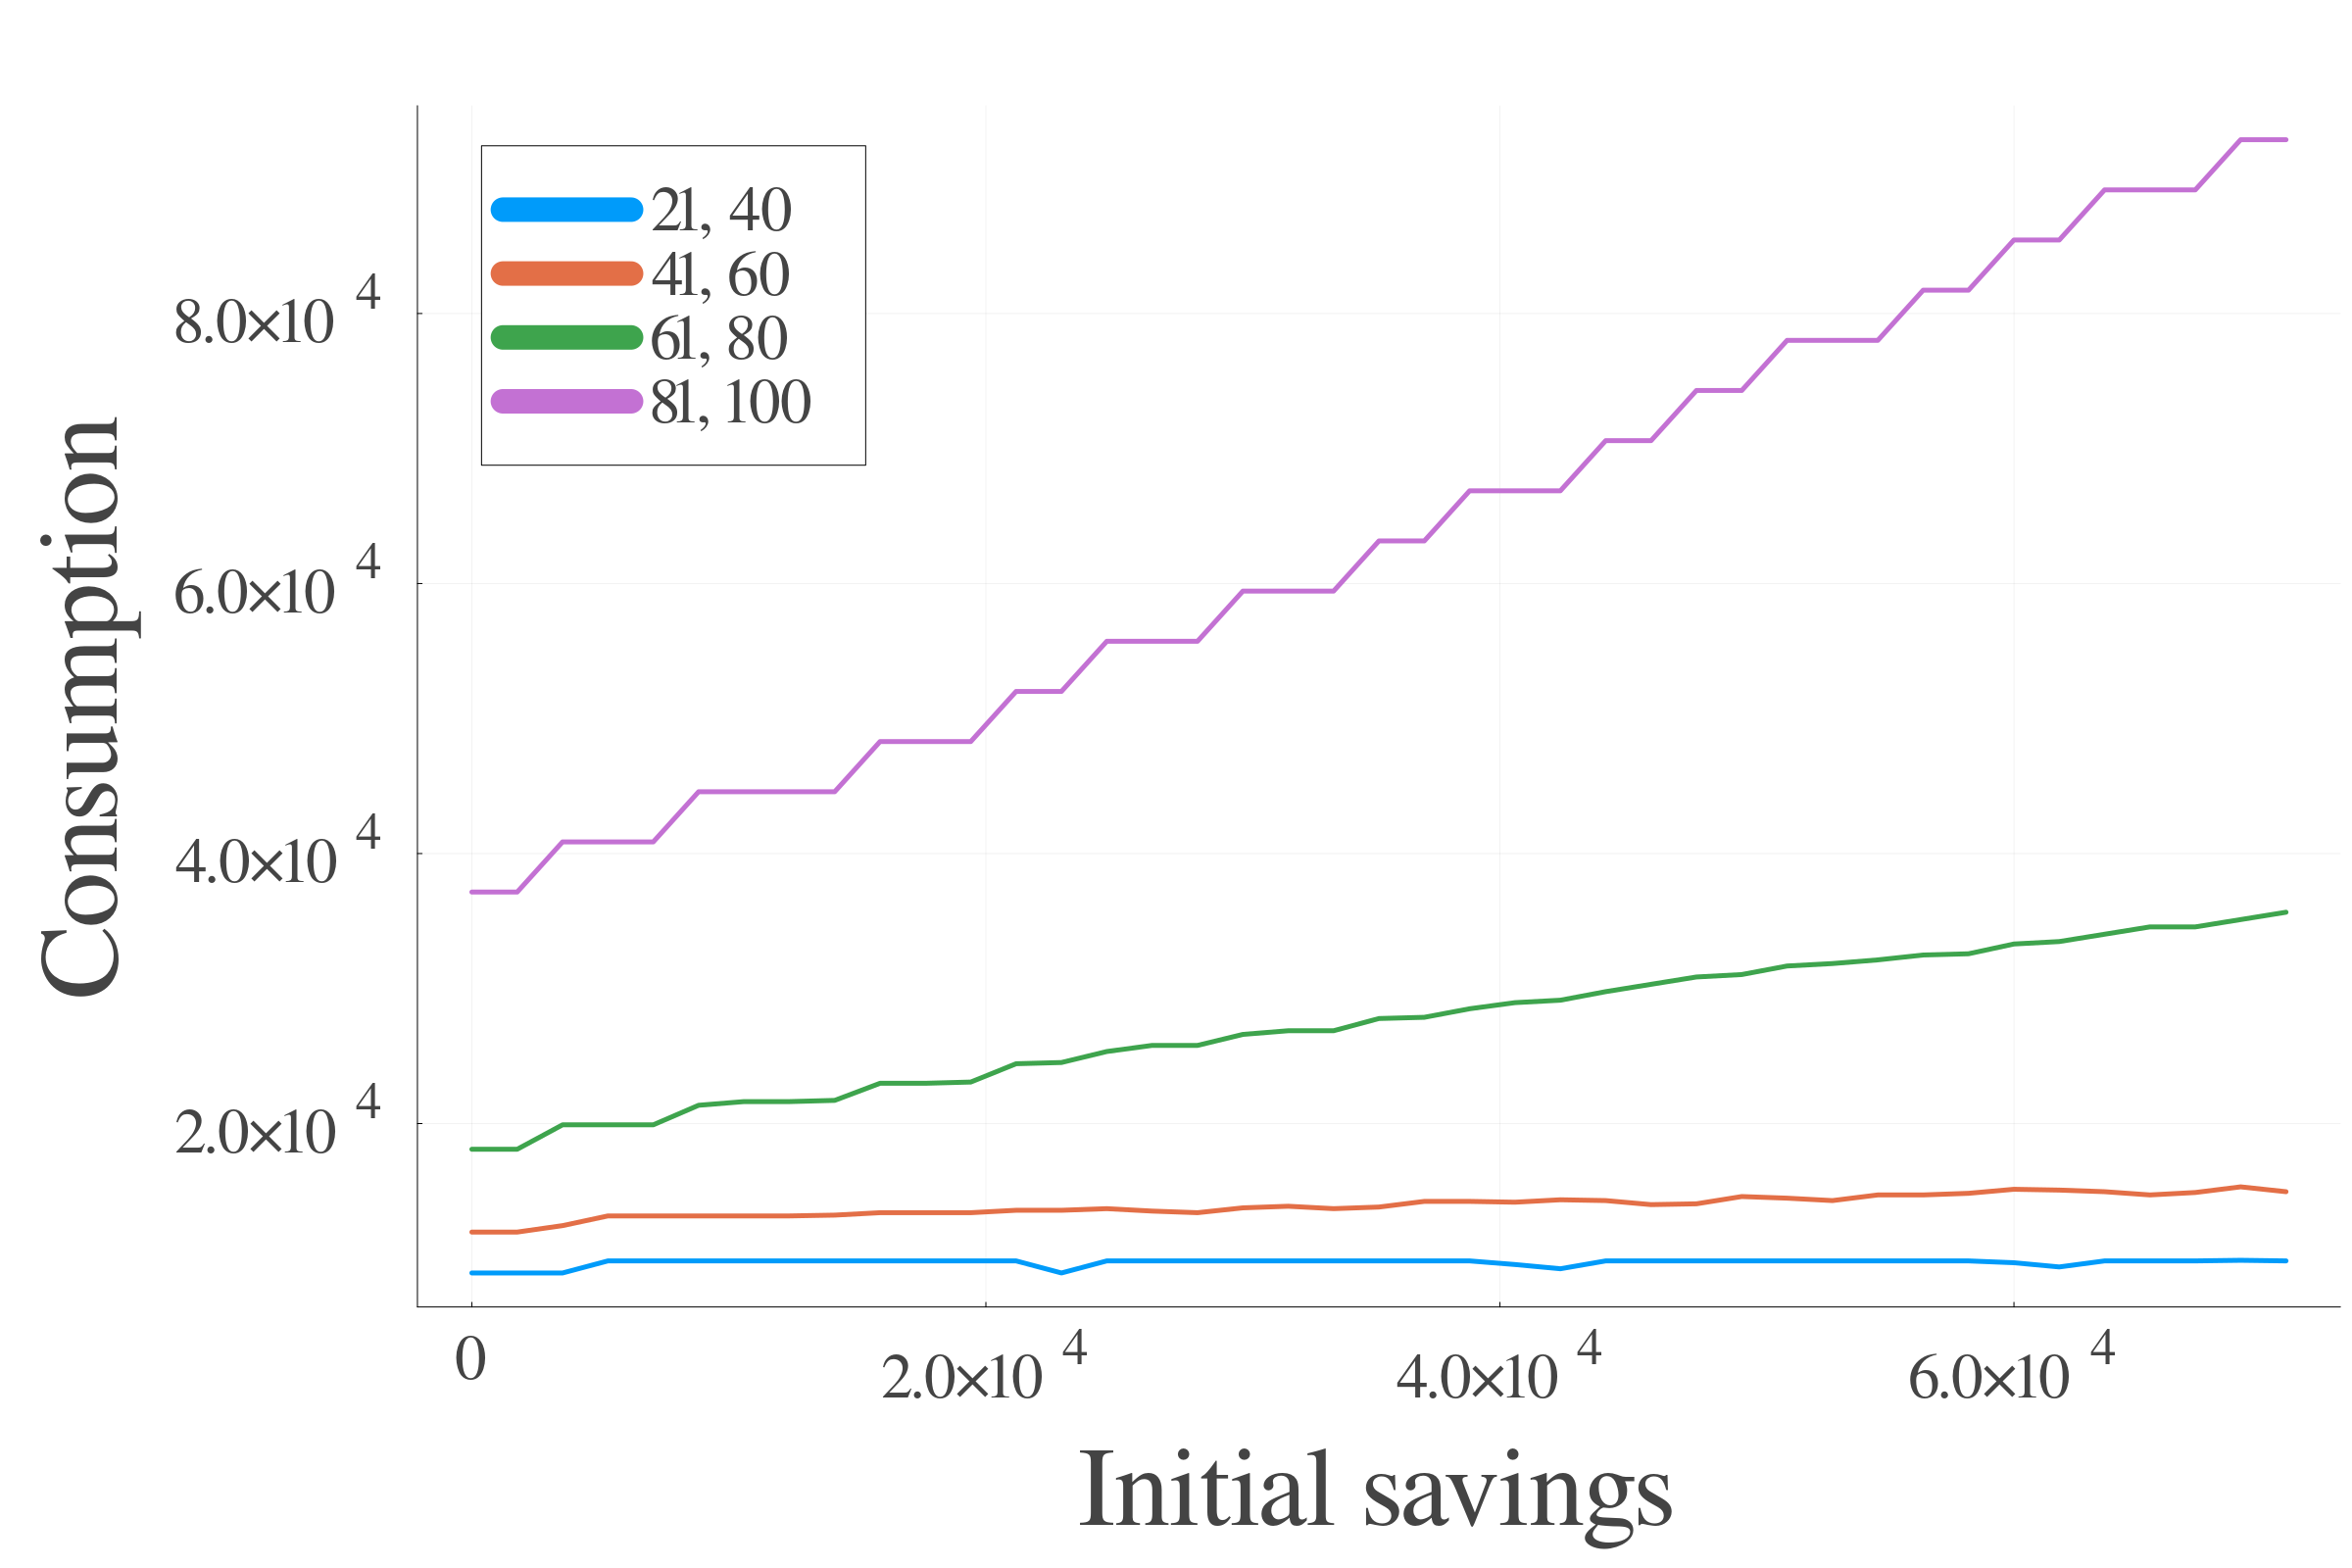
\includegraphics[width=0.7\textwidth]{/Users/paulogcd/Documents/Master_Thesis/working_elements/Draft/output/consumption_policy.png}
    \caption{Consumption policy per age category obtained from the pure numerical value function iteration}
    \label{fig:consumption_policy}
\end{figure}


The labor policy shows the increasing effect of age on
the elasticity between savings and labor income, due to
decreasing survival probabilities.

The savings policy is decreasing with age,
reflecting the lower survival probabitilies as the agents 
become older. 
In the last years, the agents desave, and tend to consume everything they have left. 


\begin{figure}[H]
    \centering
    \begin{minipage}[t]{0.45\textwidth}
        \centering
        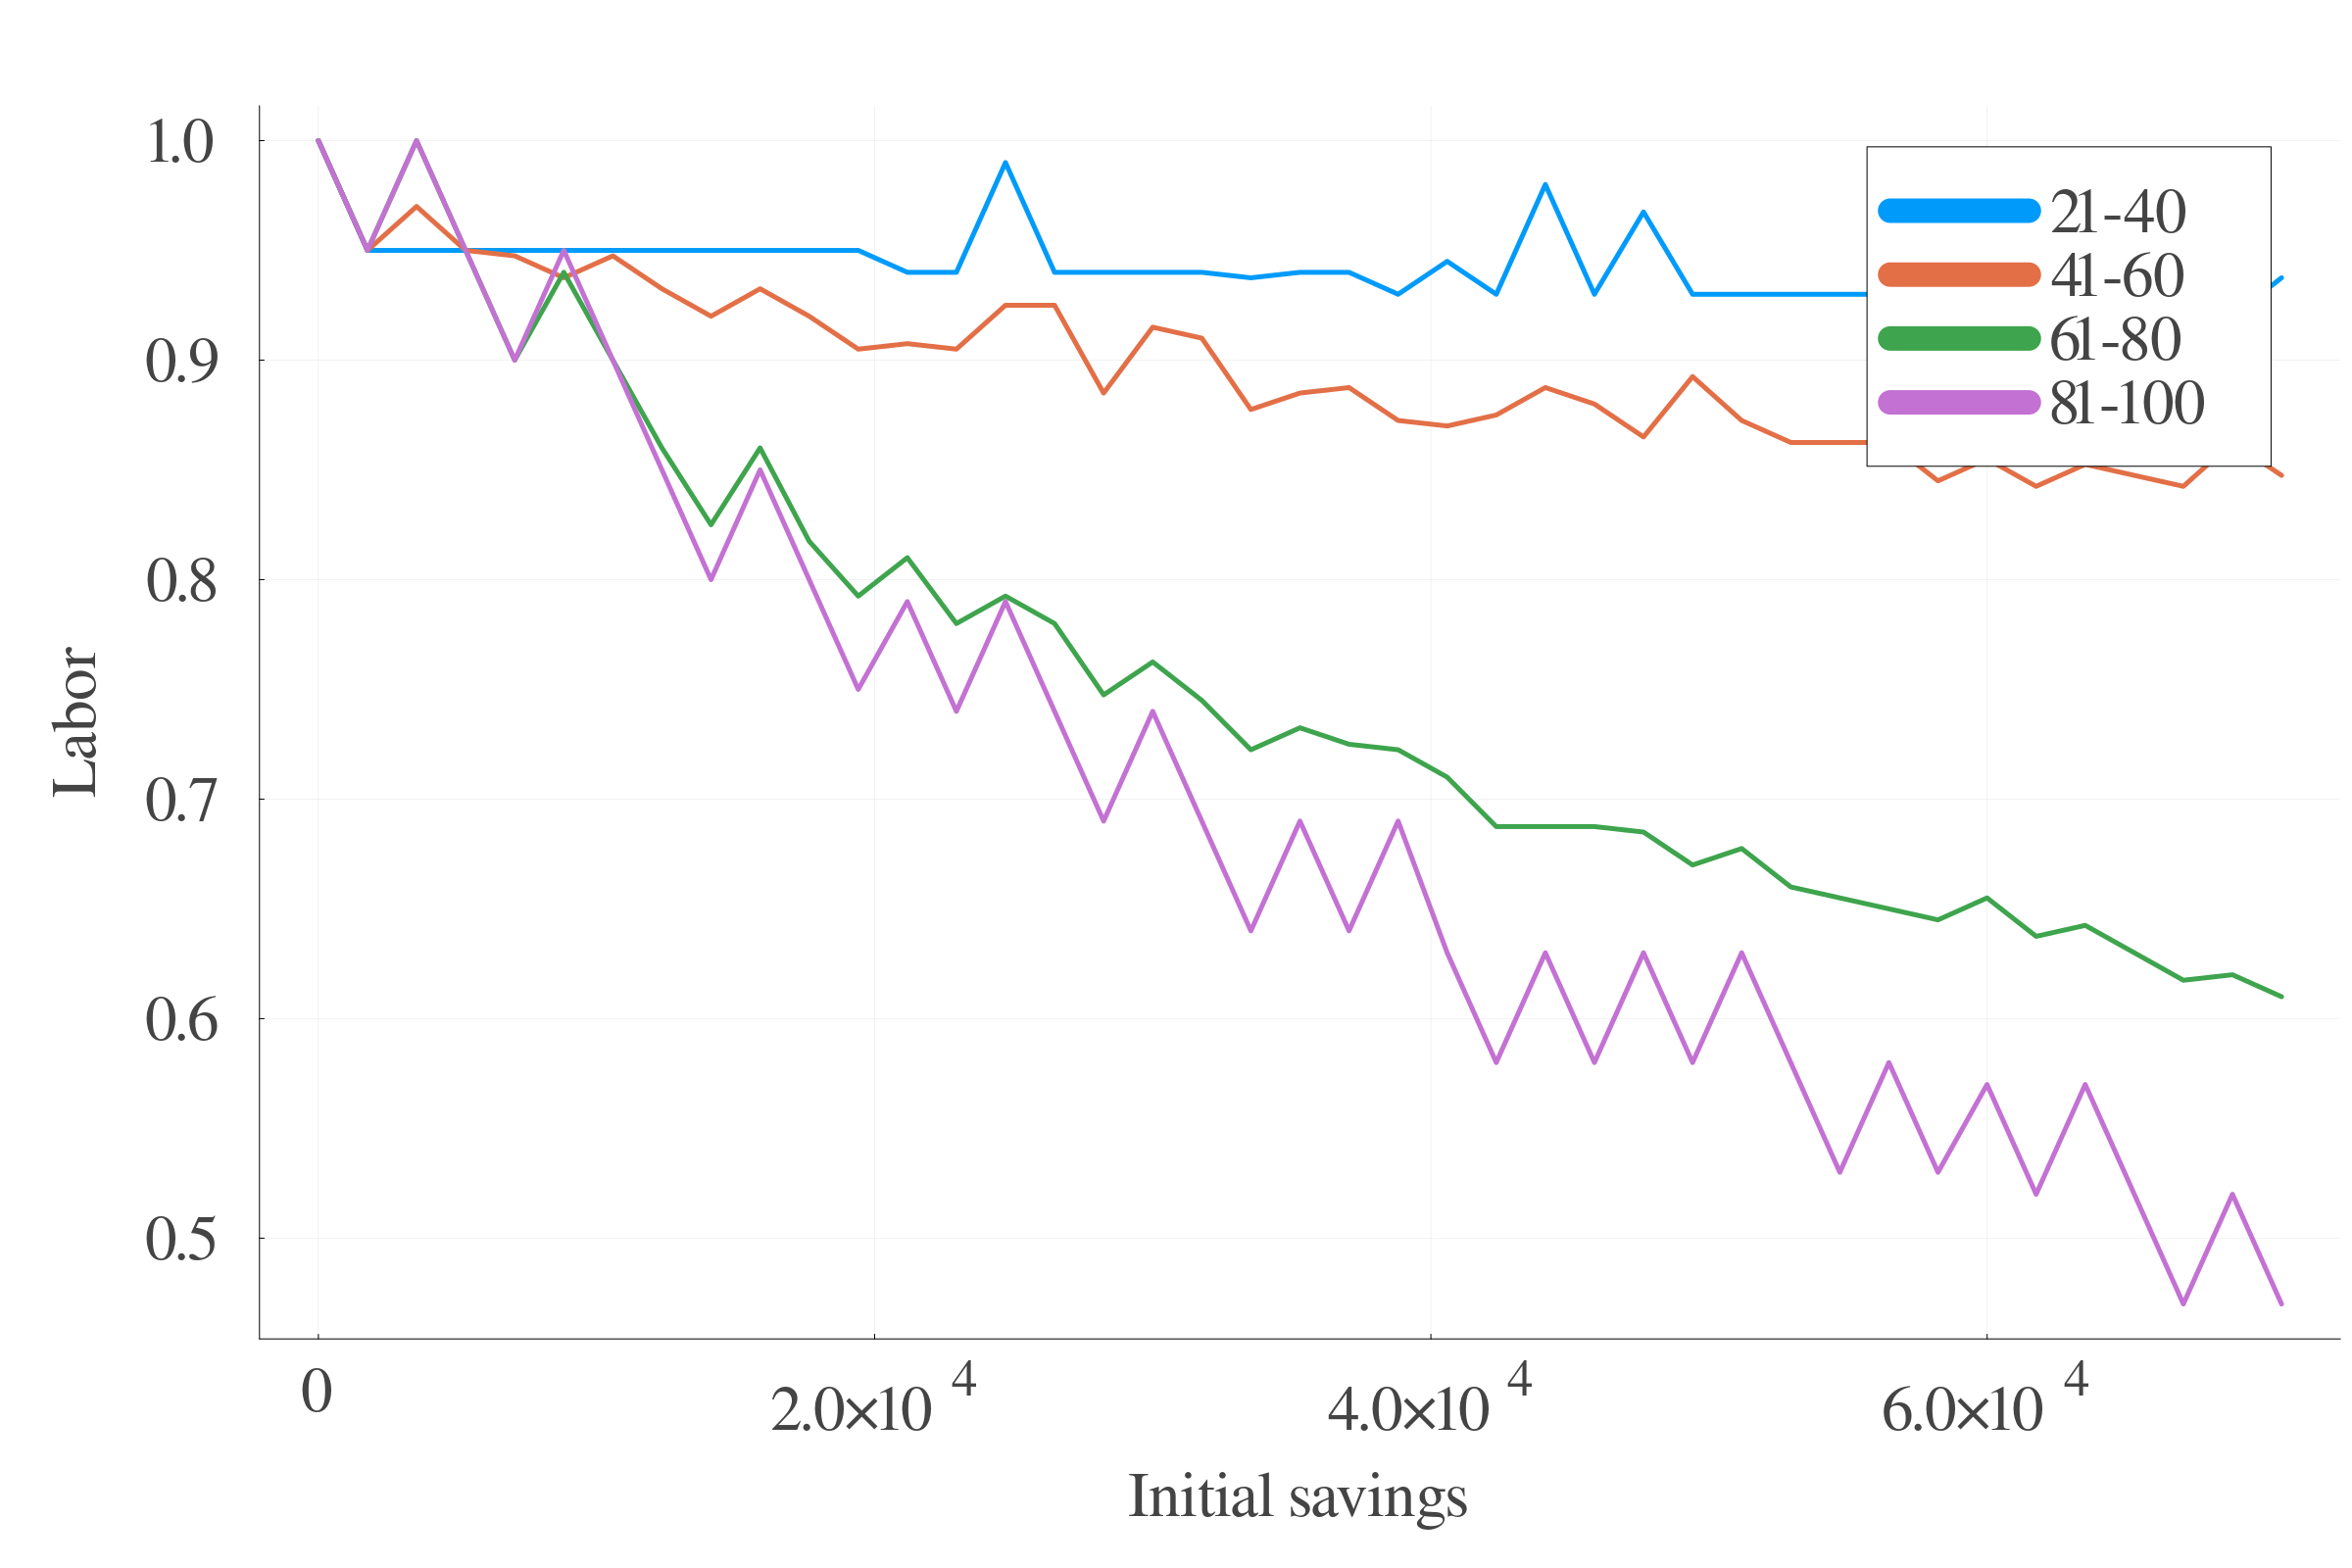
\includegraphics[width=\linewidth]{/Users/paulogcd/Documents/Master_Thesis/working_elements/Draft/output/labor_policy.png}
        \caption{Labor policy per age category}
        \label{fig:labor_policy}
    \end{minipage}
    \hfill
    \begin{minipage}[t]{0.45\textwidth}
        \centering
        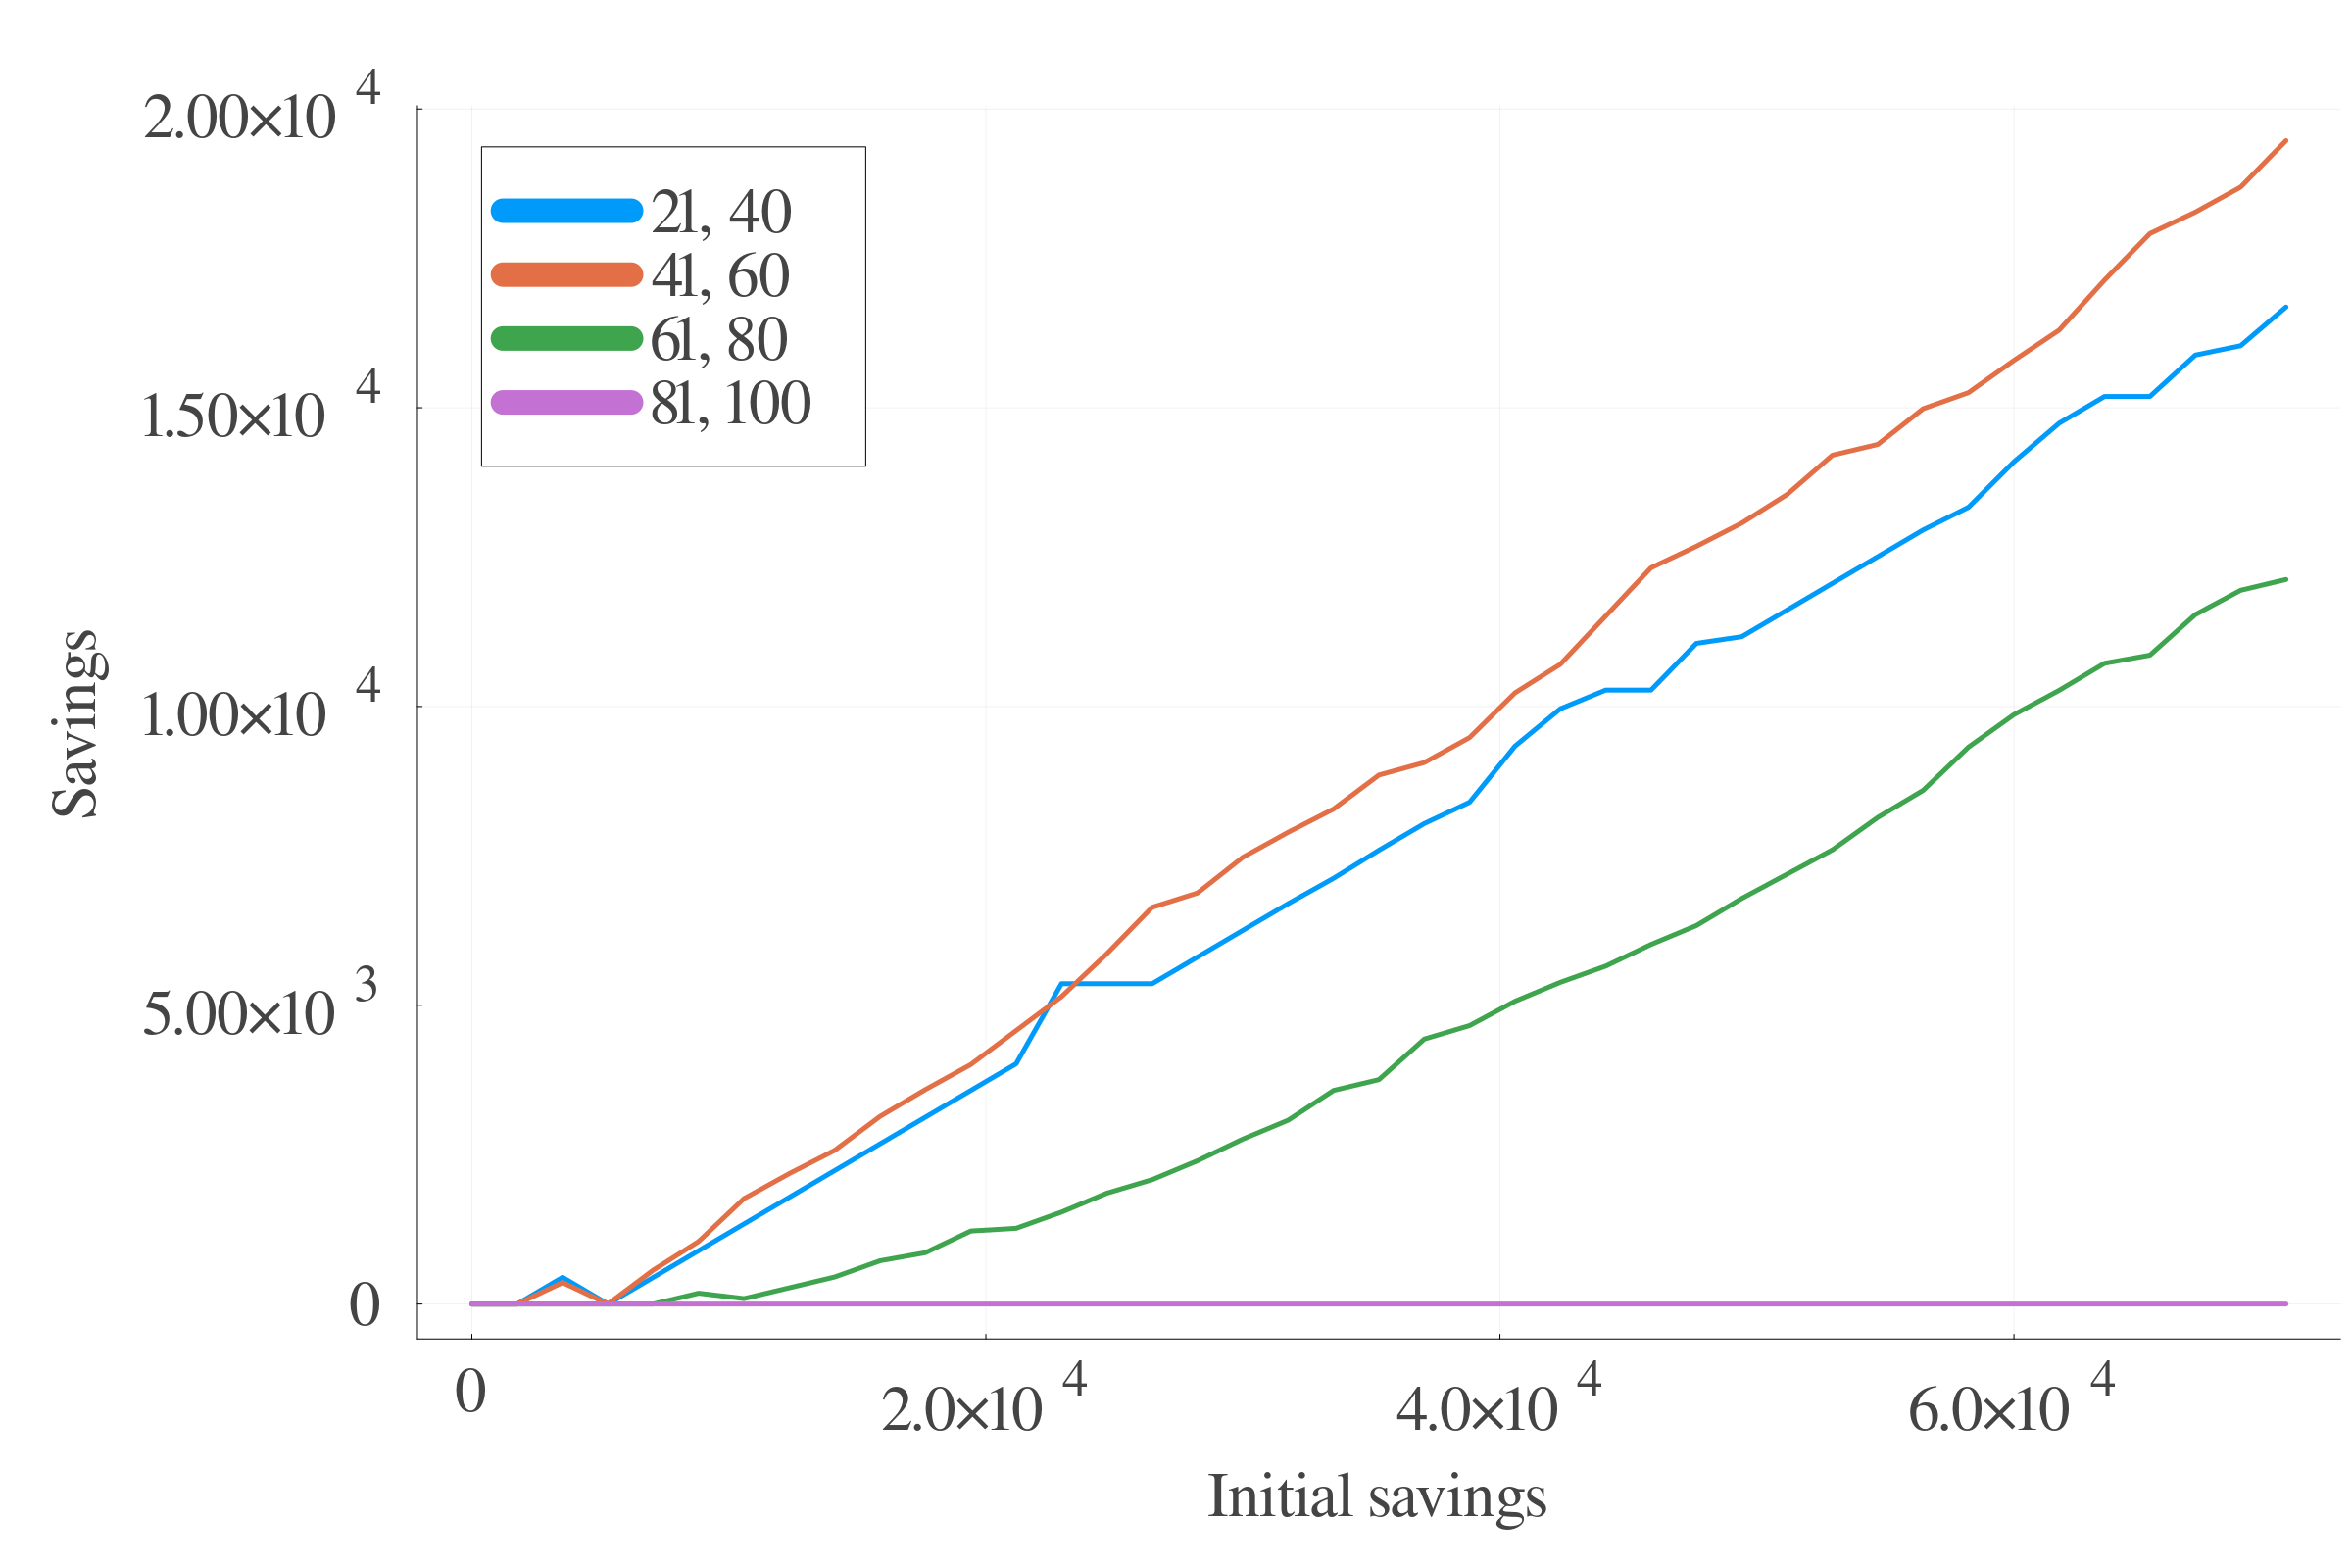
\includegraphics[width=\linewidth]{/Users/paulogcd/Documents/Master_Thesis/working_elements/Draft/output/savings_policy.png}
        \caption{Savings policy per age category}
        \label{fig:savings_policy}
    \end{minipage}
\end{figure}




\section{Results}

This section is dedicated to the presentation of the results of the comparison 
of the life time income between agents in different temperature scenarios. 

\subsection{Lifetime income}

To perform a comparison between different temperatures scenarios,
we first need to precisely characterized the comparison reference, 
i.e. the lifetime income.

A simulation was conducted using a projected temperature trajectory ranging from 0.00 to 1.50 degrees Celsius. This range approximately reflects the temperature increase experienced by the cohort born in the 1950s.

According to data from \cite{Lifetime_income}, the estimated lifetime earnings (in 2020 dollars) for individuals with less than a high school education (LTHS) are \$1,178,000 for men and \$586,000 for women, yielding an average of approximately \$882,000.
For high school graduates, the corresponding figures are \$1,825,000 for men and \$1,351,000 for women.

In light of these benchmarks, a reference value of \$1.45 million was selected to represent a moderate level of lifetime earnings. This serves as the baseline for estimating the economic consequences of temperature-related health shocks over the lifespan of this cohort.

It is important to note, however, that this estimate likely understates the true cost of such shocks. The Health and Retirement Study (HRS) data used in the health transition modeling includes a broader and more educated sample than the average LTHS population. Numerous studies have established that higher educational attainment is associated with improved health outcomes and longer life expectancy. As a result, the health impacts derived from the HRS data are expected to be less severe than those experienced by less educated individuals. Consequently, the simulated economic burden associated with temperature-induced health deterioration may be conservatively estimated.

\subsection{Comparison}

This subsection is dedicated to the comparison between 
populations having different temperature trajectories. 

First, survival probabilities will be compared, 
then, the policy functions will be compared (consumption, labor, savings). 
Finally, the lifetime income will be compared.

The 4 temperature trajectories compared are: 

\begin{itemize}
    \item The past temperature trajectory: From 0.01 to 1.5
    \item The optimistic scenario: From 0.61 to 2.0
    \item The intermediate scenario: From 0.61 to 3.0 
    \item The pessimistic scenario: From 0.61 to 4.0 
\end{itemize}

\subsubsection{Demographic comparison}

\begin{figure}[H]
    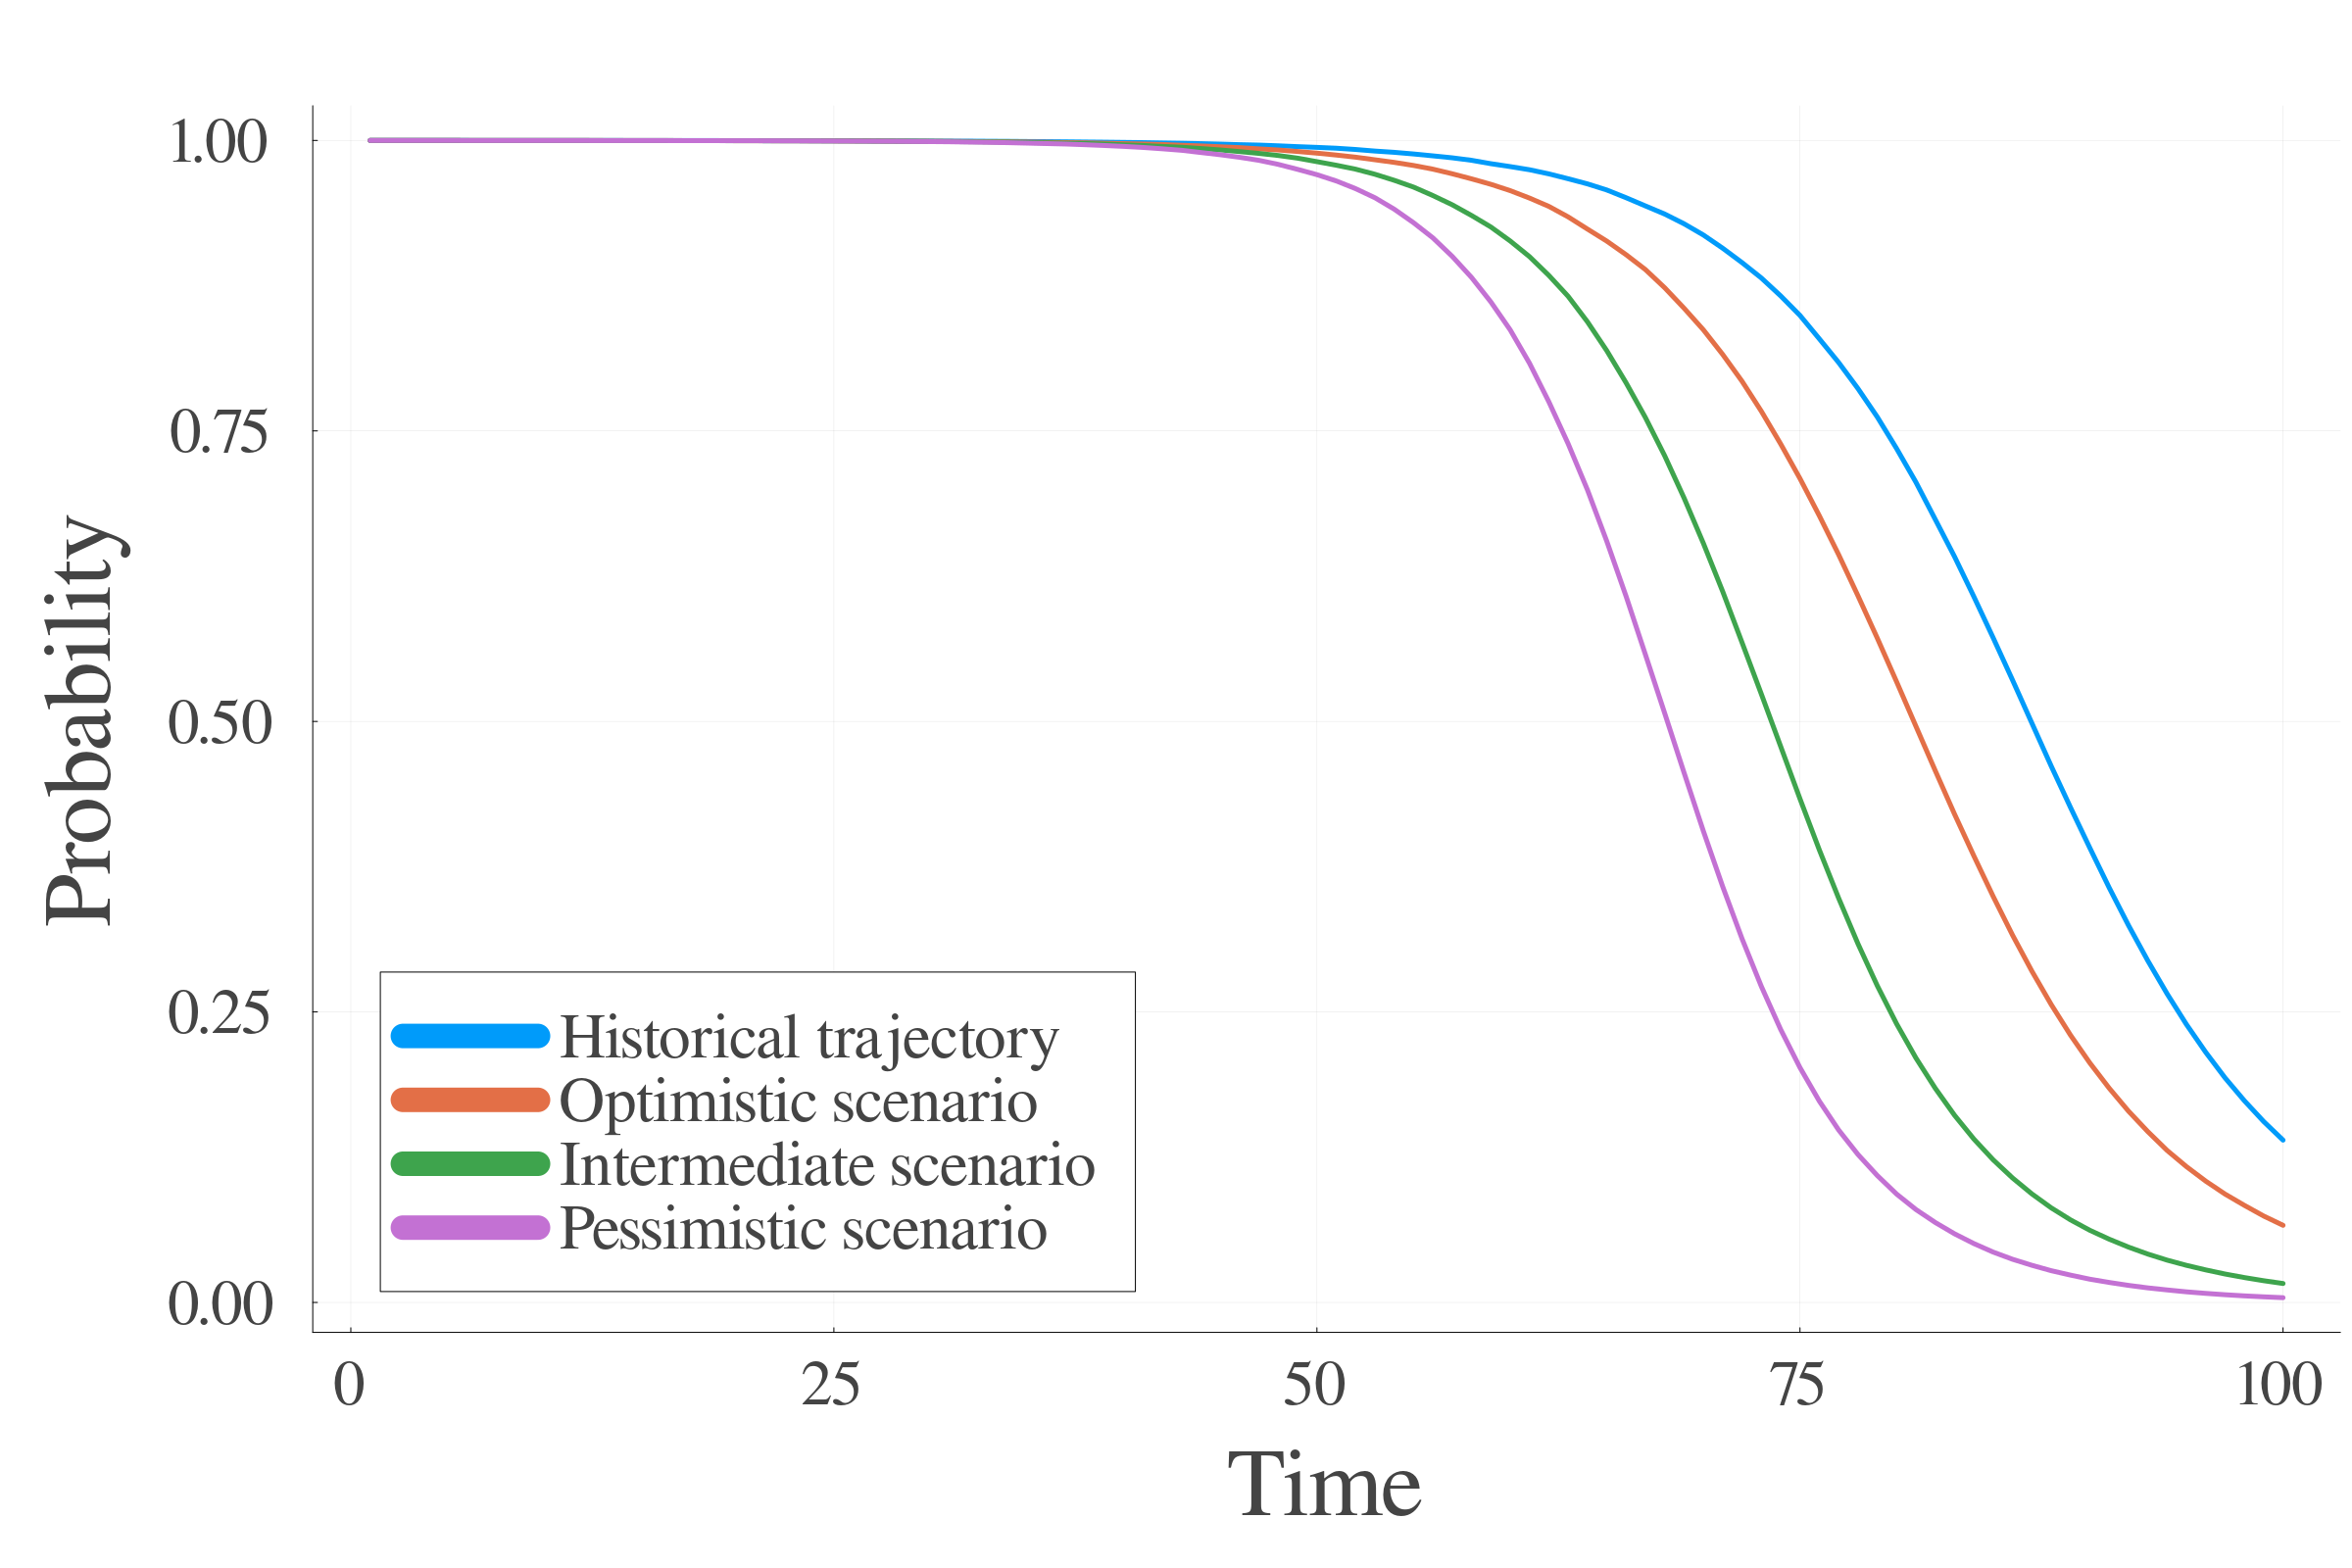
\includegraphics[width=\textwidth]{/Users/paulogcd/Documents/Master_Thesis/working_elements/Draft/output/demographic_comparison.png}
    \caption{Survival probability comparison}
\end{figure}

The following demographic comparison illustrates the heterogeneous impact of varying temperature trajectories on population survival probabilities across the life cycle.
The depicted survival curves reveal a clear downward shift and accelerated decline under more adverse climate scenarios (intermediate and pessimistic), particularly at older ages.
This suggests a significant temperature-induced mortality risk, consistent with findings in environmental epidemiology linking higher temperatures to increased incidence of acute health events and exacerbated chronic conditions.
The divergence in survival probabilities across the simulated temperature paths underscores the substantial demographic consequences of unchecked climate change, implying a contraction in expected lifespan and a potential alteration of the age structure of the population.
These demographic shifts, in turn, have profound implications for labor supply, human capital accumulation, and the sustainability of social insurance systems, as explored further in the subsequent analysis of policy functions and lifetime income.

\subsubsection{Policy functions comparison}

One possible way to compare policy functions across populations are 
the computation of a policy function average throughout all ages. 

\begin{figure}[H]
    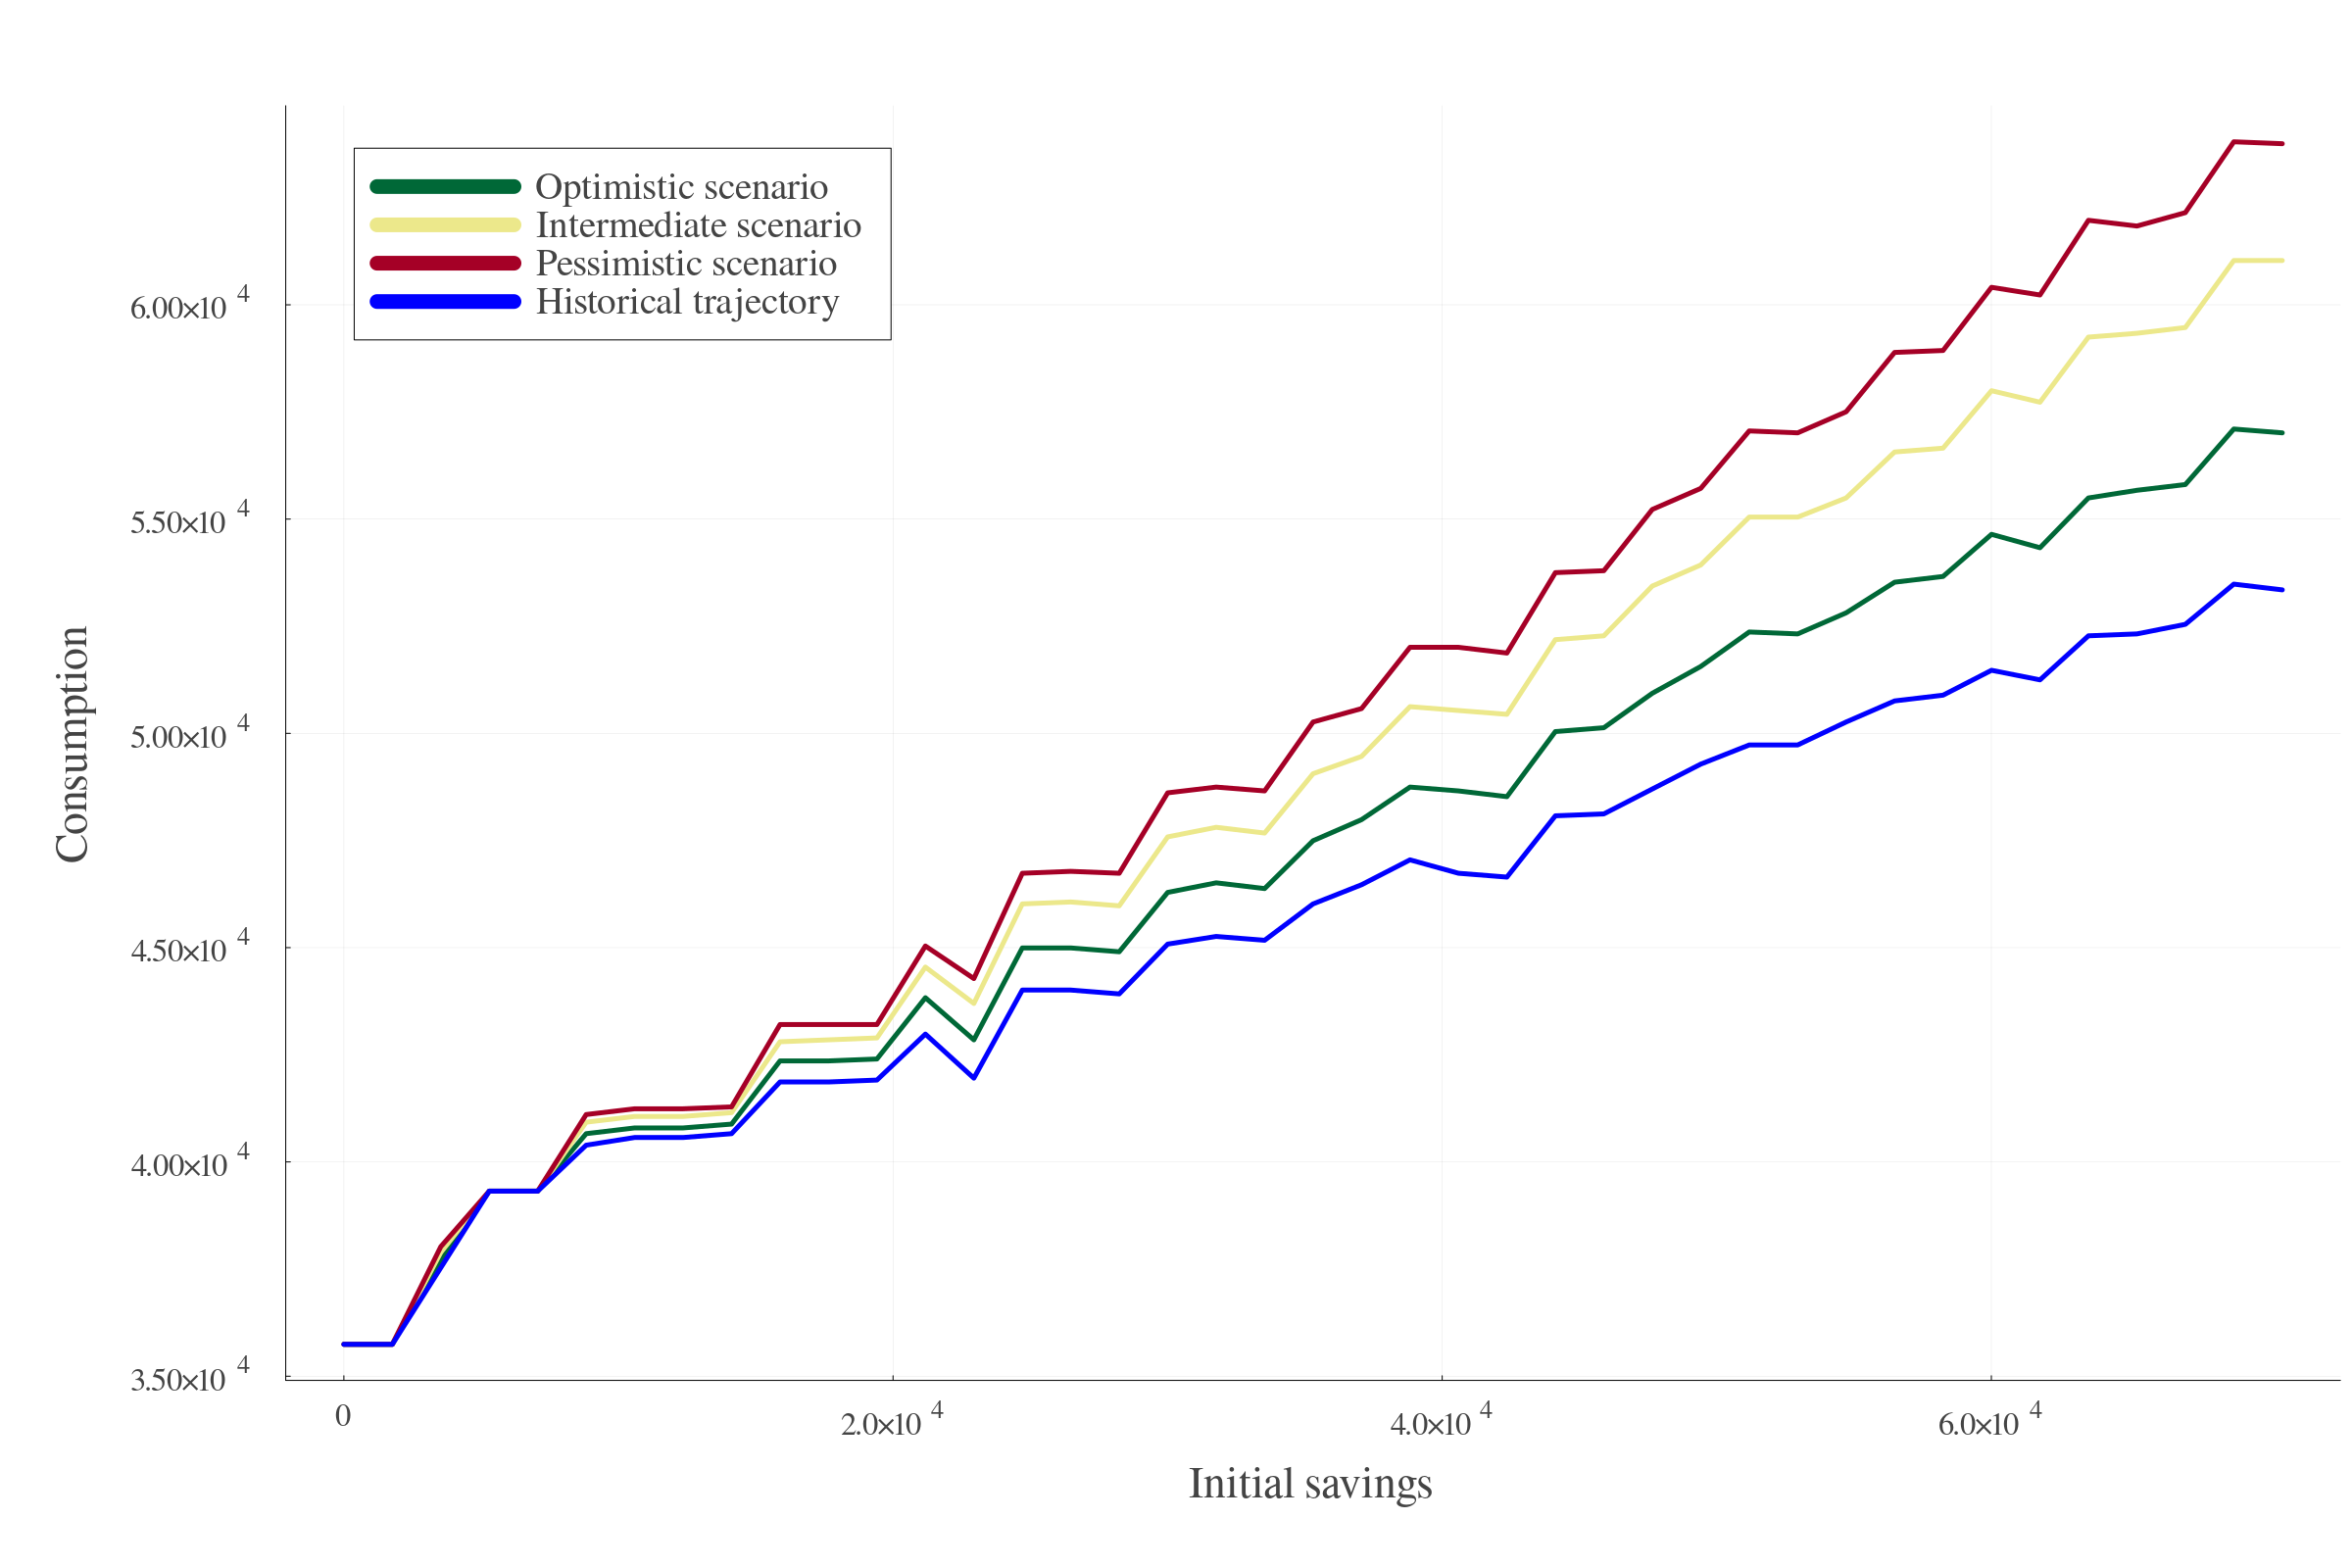
\includegraphics[width=\textwidth]{/Users/paulogcd/Documents/Master_Thesis/working_elements/Draft/output/consumption_comparison.png}
    \caption{Consumption policy comparison}
\end{figure}

\begin{figure}[H]
    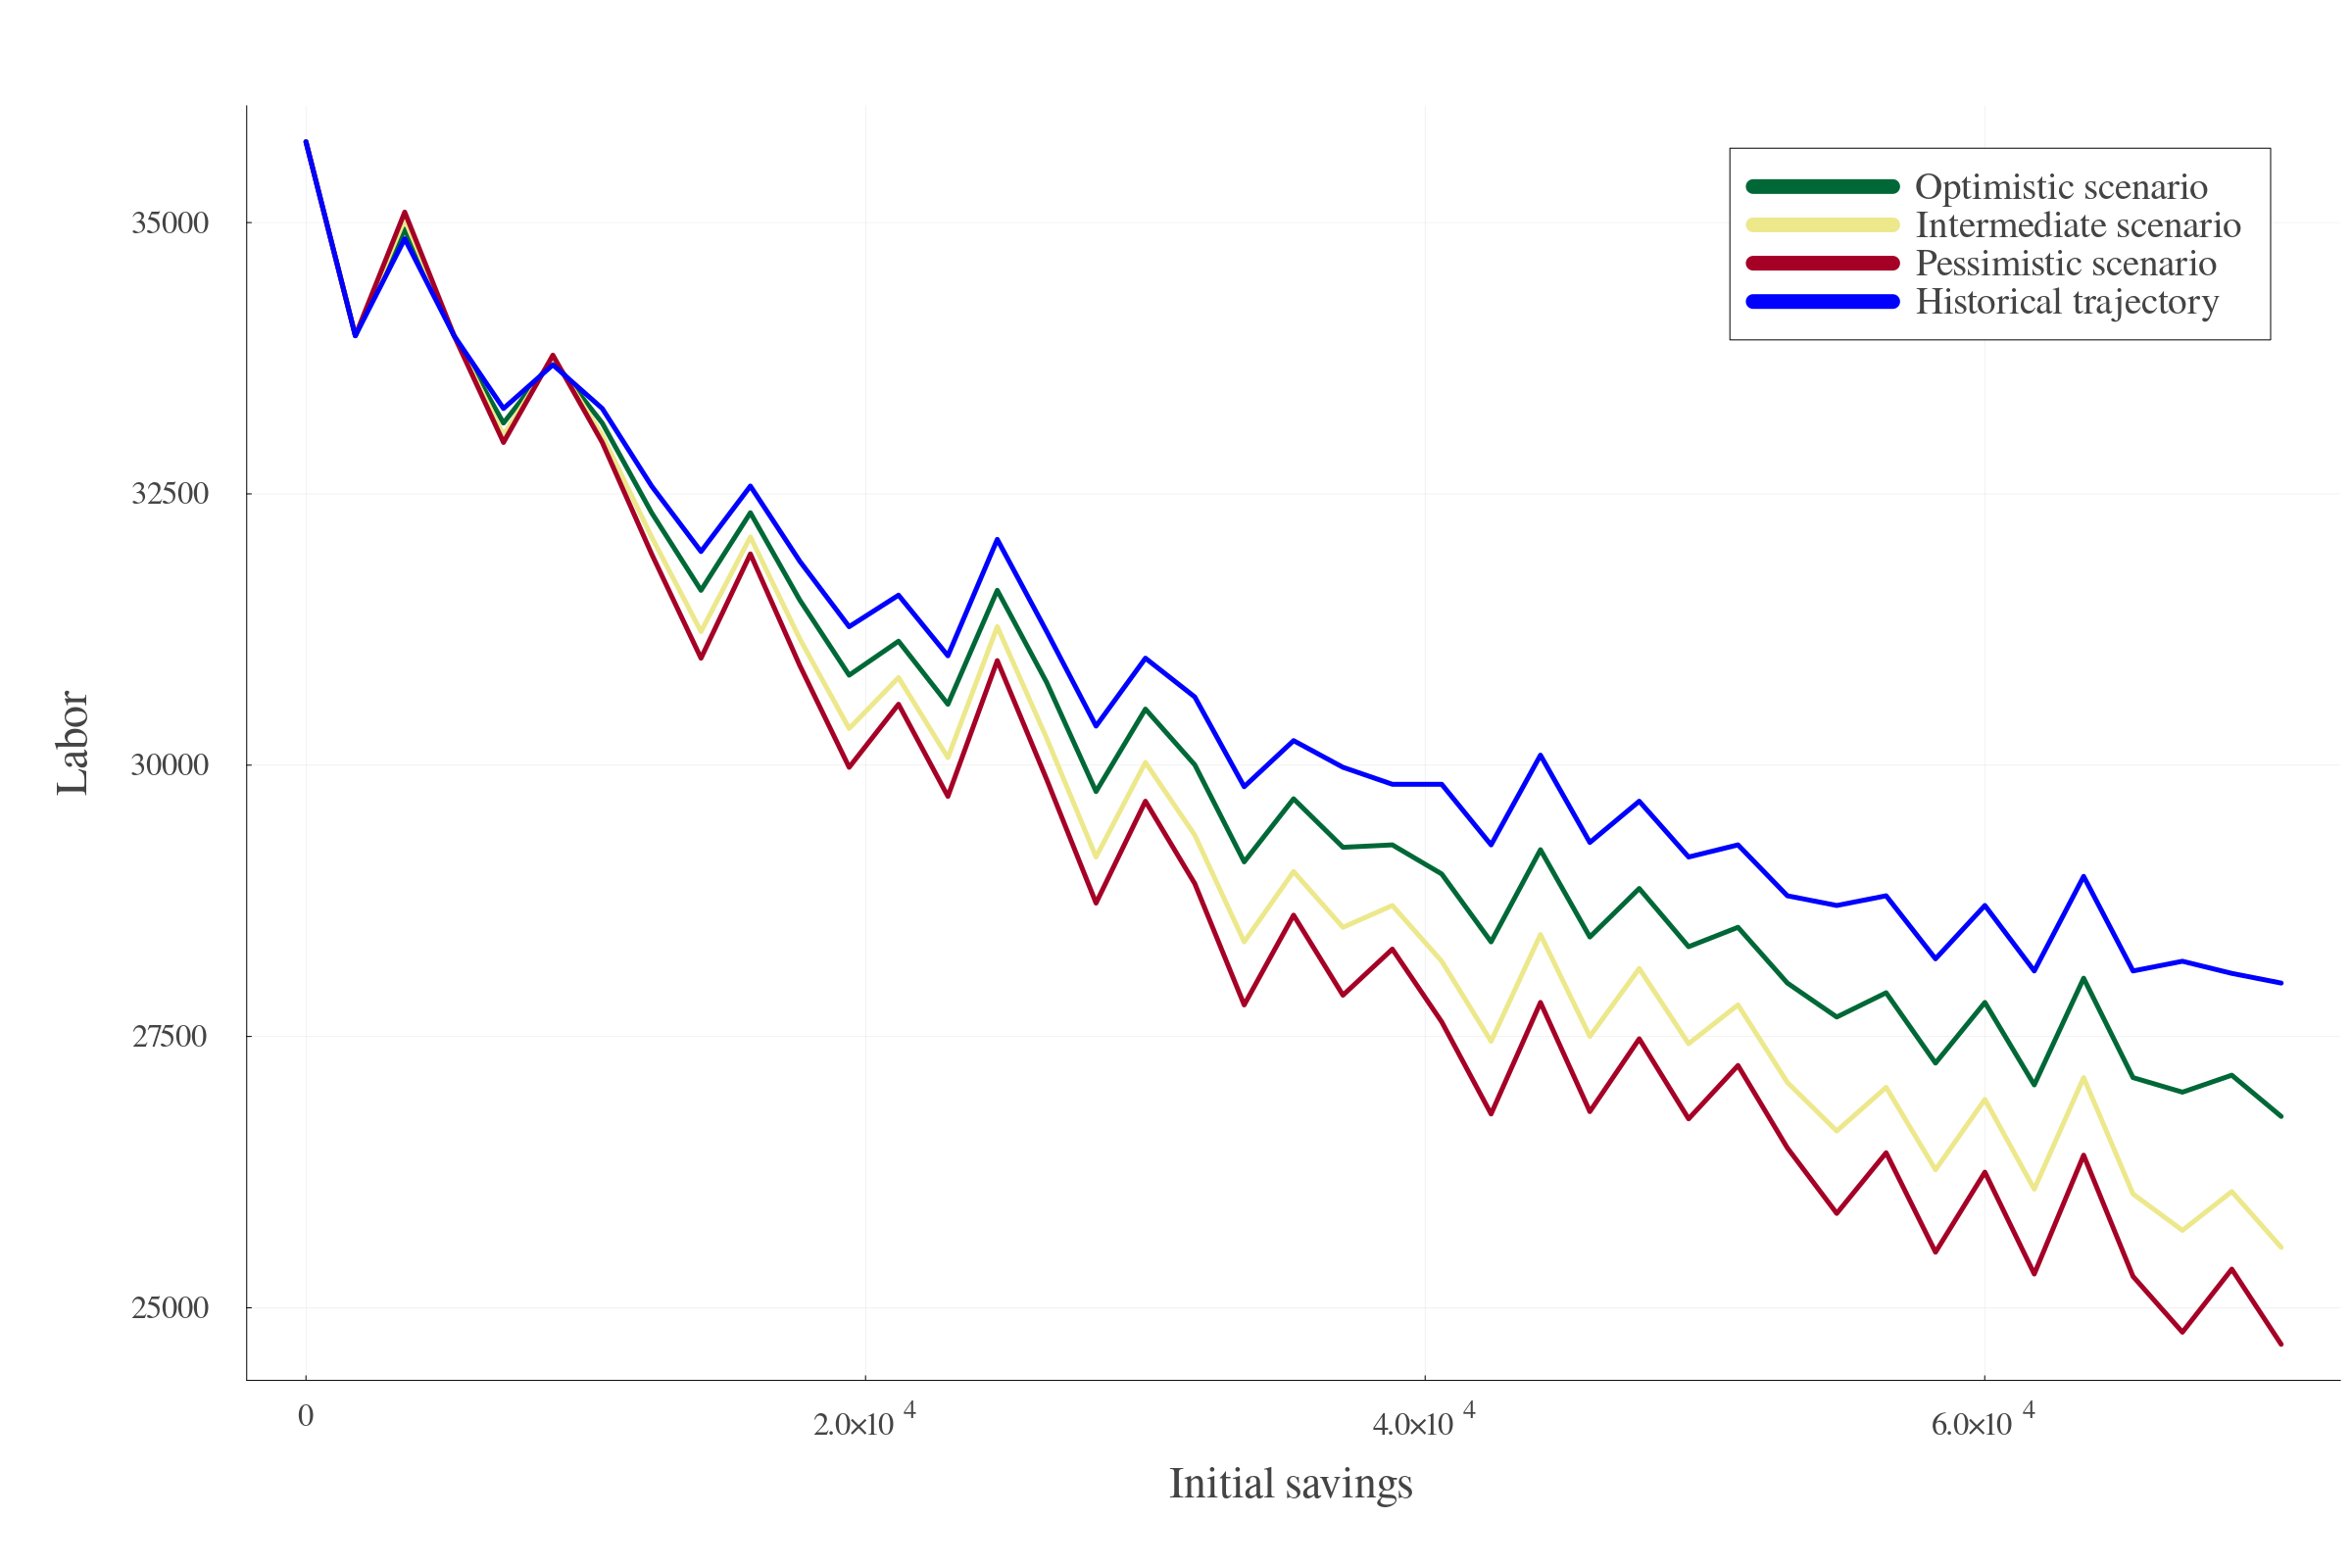
\includegraphics[width=\textwidth]{/Users/paulogcd/Documents/Master_Thesis/working_elements/Draft/output/labor_comparison.png}
    \caption{Labor policy comparison}
\end{figure}

The comparison of optimal policy paths across varying temperature trajectories reveals a discernible loss attributable to demographic dynamics.
Specifically, this loss arises from temperature-induced shifts in survival probabilities over time.
As higher temperatures adversely affect health transitions and increase mortality risk (particularly among older or more vulnerable individuals) the resulting demographic structure alters the expected lifetime utility and economic behavior of agents.

This demographic distortion reduces the effectiveness of policy instruments optimized under baseline conditions, thereby generating inefficiencies.
The magnitude of the loss reflects both the direct impact of elevated temperatures on survival probabilities and the indirect effect on population composition, labor force participation, and the intertemporal allocation of resources. In this context, the demographic channel becomes a critical mechanism through which climate change translates into long-term economic costs, even in the absence of immediate productivity shocks.

\subsubsection{Lifetime income comparison}

The deterioration in lifetime income resulting from temperature-related health shocks is substantial and operates through multiple, compounding channels. Elevated temperatures are empirically associated with a higher incidence of acute health events—such as cardiovascular and respiratory crises—that not only increase short-term morbidity and mortality but also reduce long-term functional capacity. These effects are particularly pronounced among older adults and individuals in fragile health, whose ability to remain in the labor force or engage in productive activities declines disproportionately.

\begin{figure}[H]
    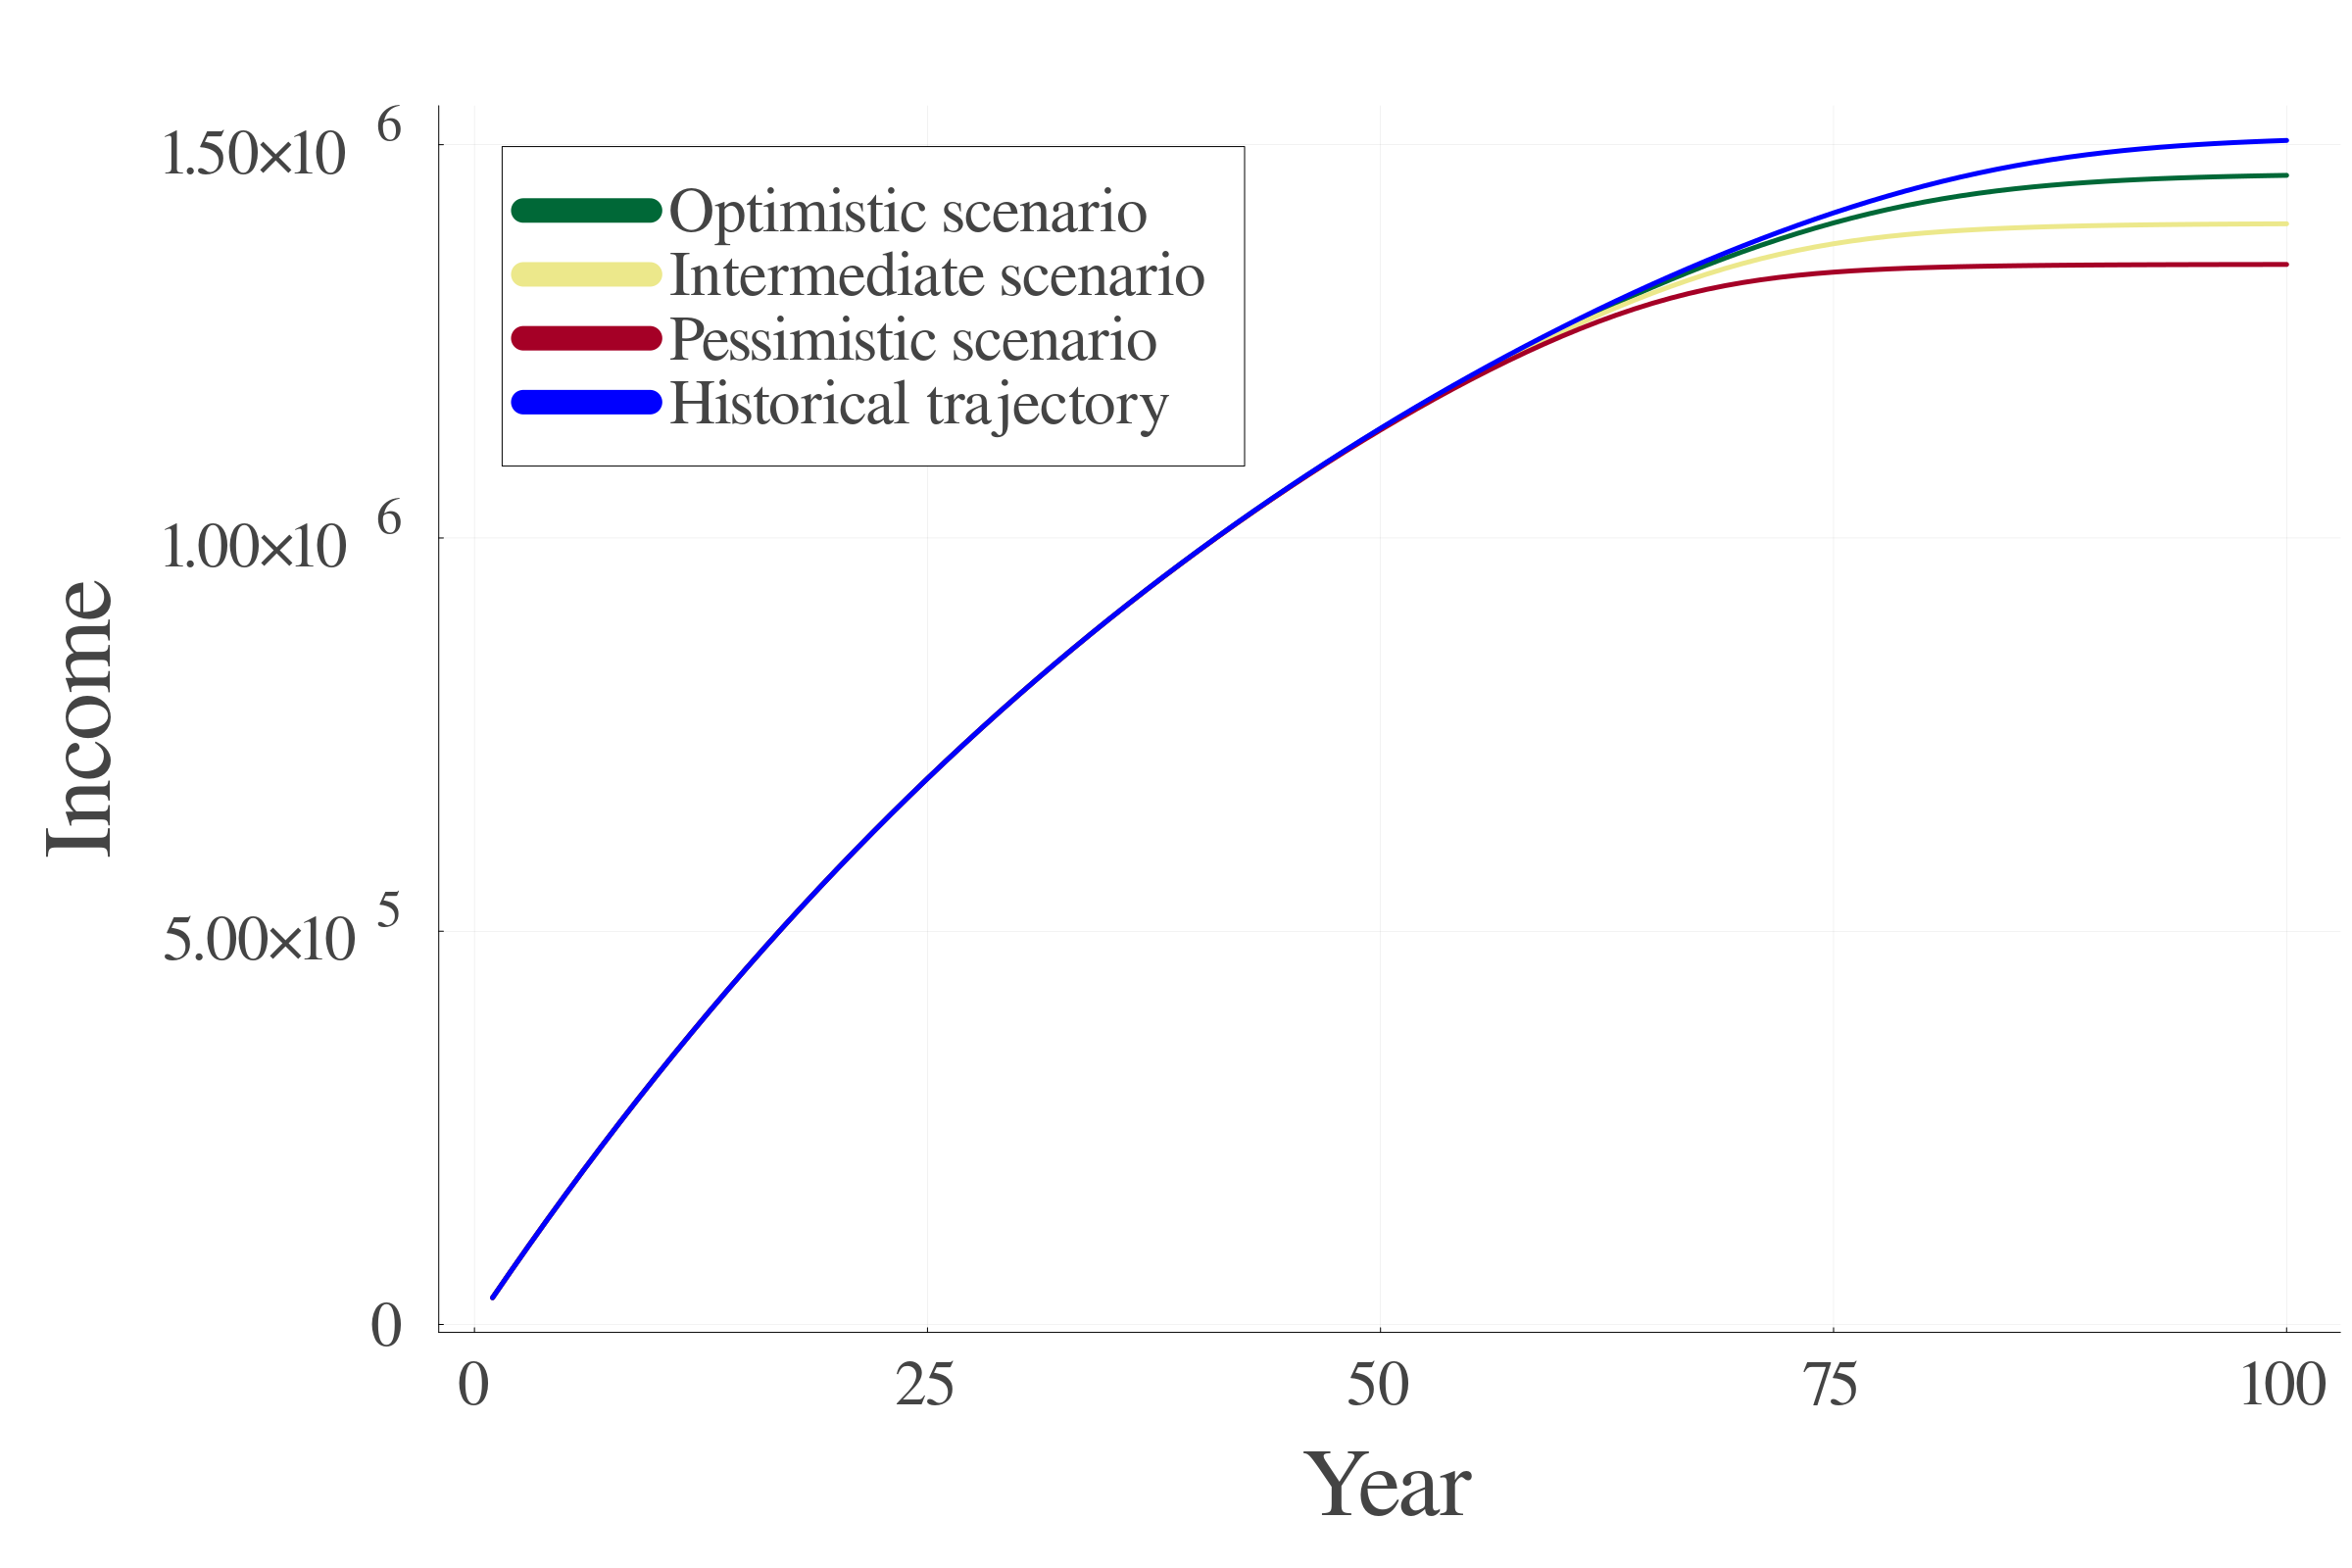
\includegraphics[width=\textwidth]{/Users/paulogcd/Documents/Master_Thesis/working_elements/Draft/output/lifetime_income_comparison.png}
    \caption{Expected lifetime labor income, at each period.}
\end{figure}

Simulations suggest that even modest increases in average temperature over the life course can translate into significant reductions in expected lifetime income.
This arises not only from premature mortality but also from suboptimal health states that lower utility and earning potential throughout the individual’s remaining life. Therefore, the macroeconomic cost of climate-related health deterioration should be understood as not merely a public health challenge but a fundamental constraint on human capital and economic resilience.
In this sense, the lifetime income loss induced by change in survival probabilities due to acute health conditions provoked by temperature changes amounts to approximately \$110,000 of 2020, when taking the lifetime income of the High School Graduates of the 1950s generation (\$1.45 Mio) as the reference point.

\section{Discussion}

This paper quantifies the lifetime economic cost of temperature-induced health deterioration by integrating empirical estimates of health and survival dynamics into a structural life-cycle model. The results highlight two key mechanisms: (1) temperature-driven health shocks reduce survival probabilities, particularly among older and vulnerable populations, and (2) these shocks propagate through individual adjustments in labor supply, savings, and consumption, culminating in significant lifetime income losses (approximately \$110,000 per capita under pessimistic warming scenarios).

The estimated policy functions align with life-cycle theory: savings peak in mid-life and decumulate with age, while labor supply declines as health deteriorates.
This attempts to complement the literature on climate-economy feedbacks (Burke et al., 2015; Bilal \& Kanzig, 2024) by isolating the role of health-mediated channels absent collective adaptation.

The empirical health transitions, estimated via a two-stage ordered-response framework, confirm that temperature exacerbates acute conditions (e.g., cardiovascular stress) and accelerates transitions to poorer health states.
This mirrors findings by Barreca et al. (2016) on temperature-mortality adaptation but extends them to the economic individual choices.

\subsection{Limitations}

Nonetheless, this present work suffers from multiple methodological limitations.

First, by its econometrical strategy to assess the relationships between health, temperature, and survival.
Nordhaus called Climate Change "The Ultimate Challenge for Economics" \citep{Nordhaus_2019}, did the current work manage to tackle it? 
Needless to say, the econometric strategy of the current work is far from being flawless.
The use of two estimates in the detailed three stages regression approach still does not eliminate estimation bias.

Two other elements add up to the inherent econometric hurdle of temperature causal inference 
First, due to the reliance on the Self-Reported Health.
This reliance may understate severe clinical conditions.
Future work could integrate biomarkers (e.g., NHANES data) to capture latent health risks.
Second, due to the limitations of the proposed and used Health Proxy,
that does not capture fully neither isolate perfectly the effect of temperature on health.

At this stage, it is important to acknowledge that, while the proposed estimation strategy may be subject to bias and potential collinearity with omitted variables, it nonetheless serves a meaningful purpose within the context of the model. Although establishing strict causal inference is constrained by data limitations and identification challenges, the estimated relationships still offer valuable descriptive insights into the dynamics between temperature and health outcomes. In this regard, the economic model built upon these estimators provides a credible framework for exploring and quantifying the broader economic consequences of temperature-induced health shocks. Rather than seeking definitive causal claims, the model emphasizes the structural and behavioral implications of observed patterns, thereby offering a clearer understanding of how environmental stressors translate into long-term economic costs.

Another important limitation of this work comes from its integration of temperature variability:
Using annual averages masks acute shocks (e.g., heatwaves), which may have nonlinear effects on health (IPCC, 2022).
High-frequency data could refine the health proxy.

The third major flaw of this work is its abstraction from general equilibrium effects (e.g., wage adjustments, health investment).
A richer framework could include endogenous labor demand or public adaptation policies.

Finally, it could be interesting to introduce educational heterogeneity for two reasons. 
Not only would it create heterogeneity at the productivity level, but it would also interact with 
the health and survival probabilities.
Furthermore, the baseline lifetime income estimate (\$1.45M) likely understates costs for less-educated groups, who face higher climate vulnerability (Deryugina \& Hsiang, 2017).
Disaggregating by socioeconomic status could be a priority for future research.

\section{References}

\printbibliography[heading=none]

\newpage
\section{Appendix}

\subsection{Health Transition Probabilities}

\begin{figure}[H]\label{fig:health_transition_2}
    \begin{center}
        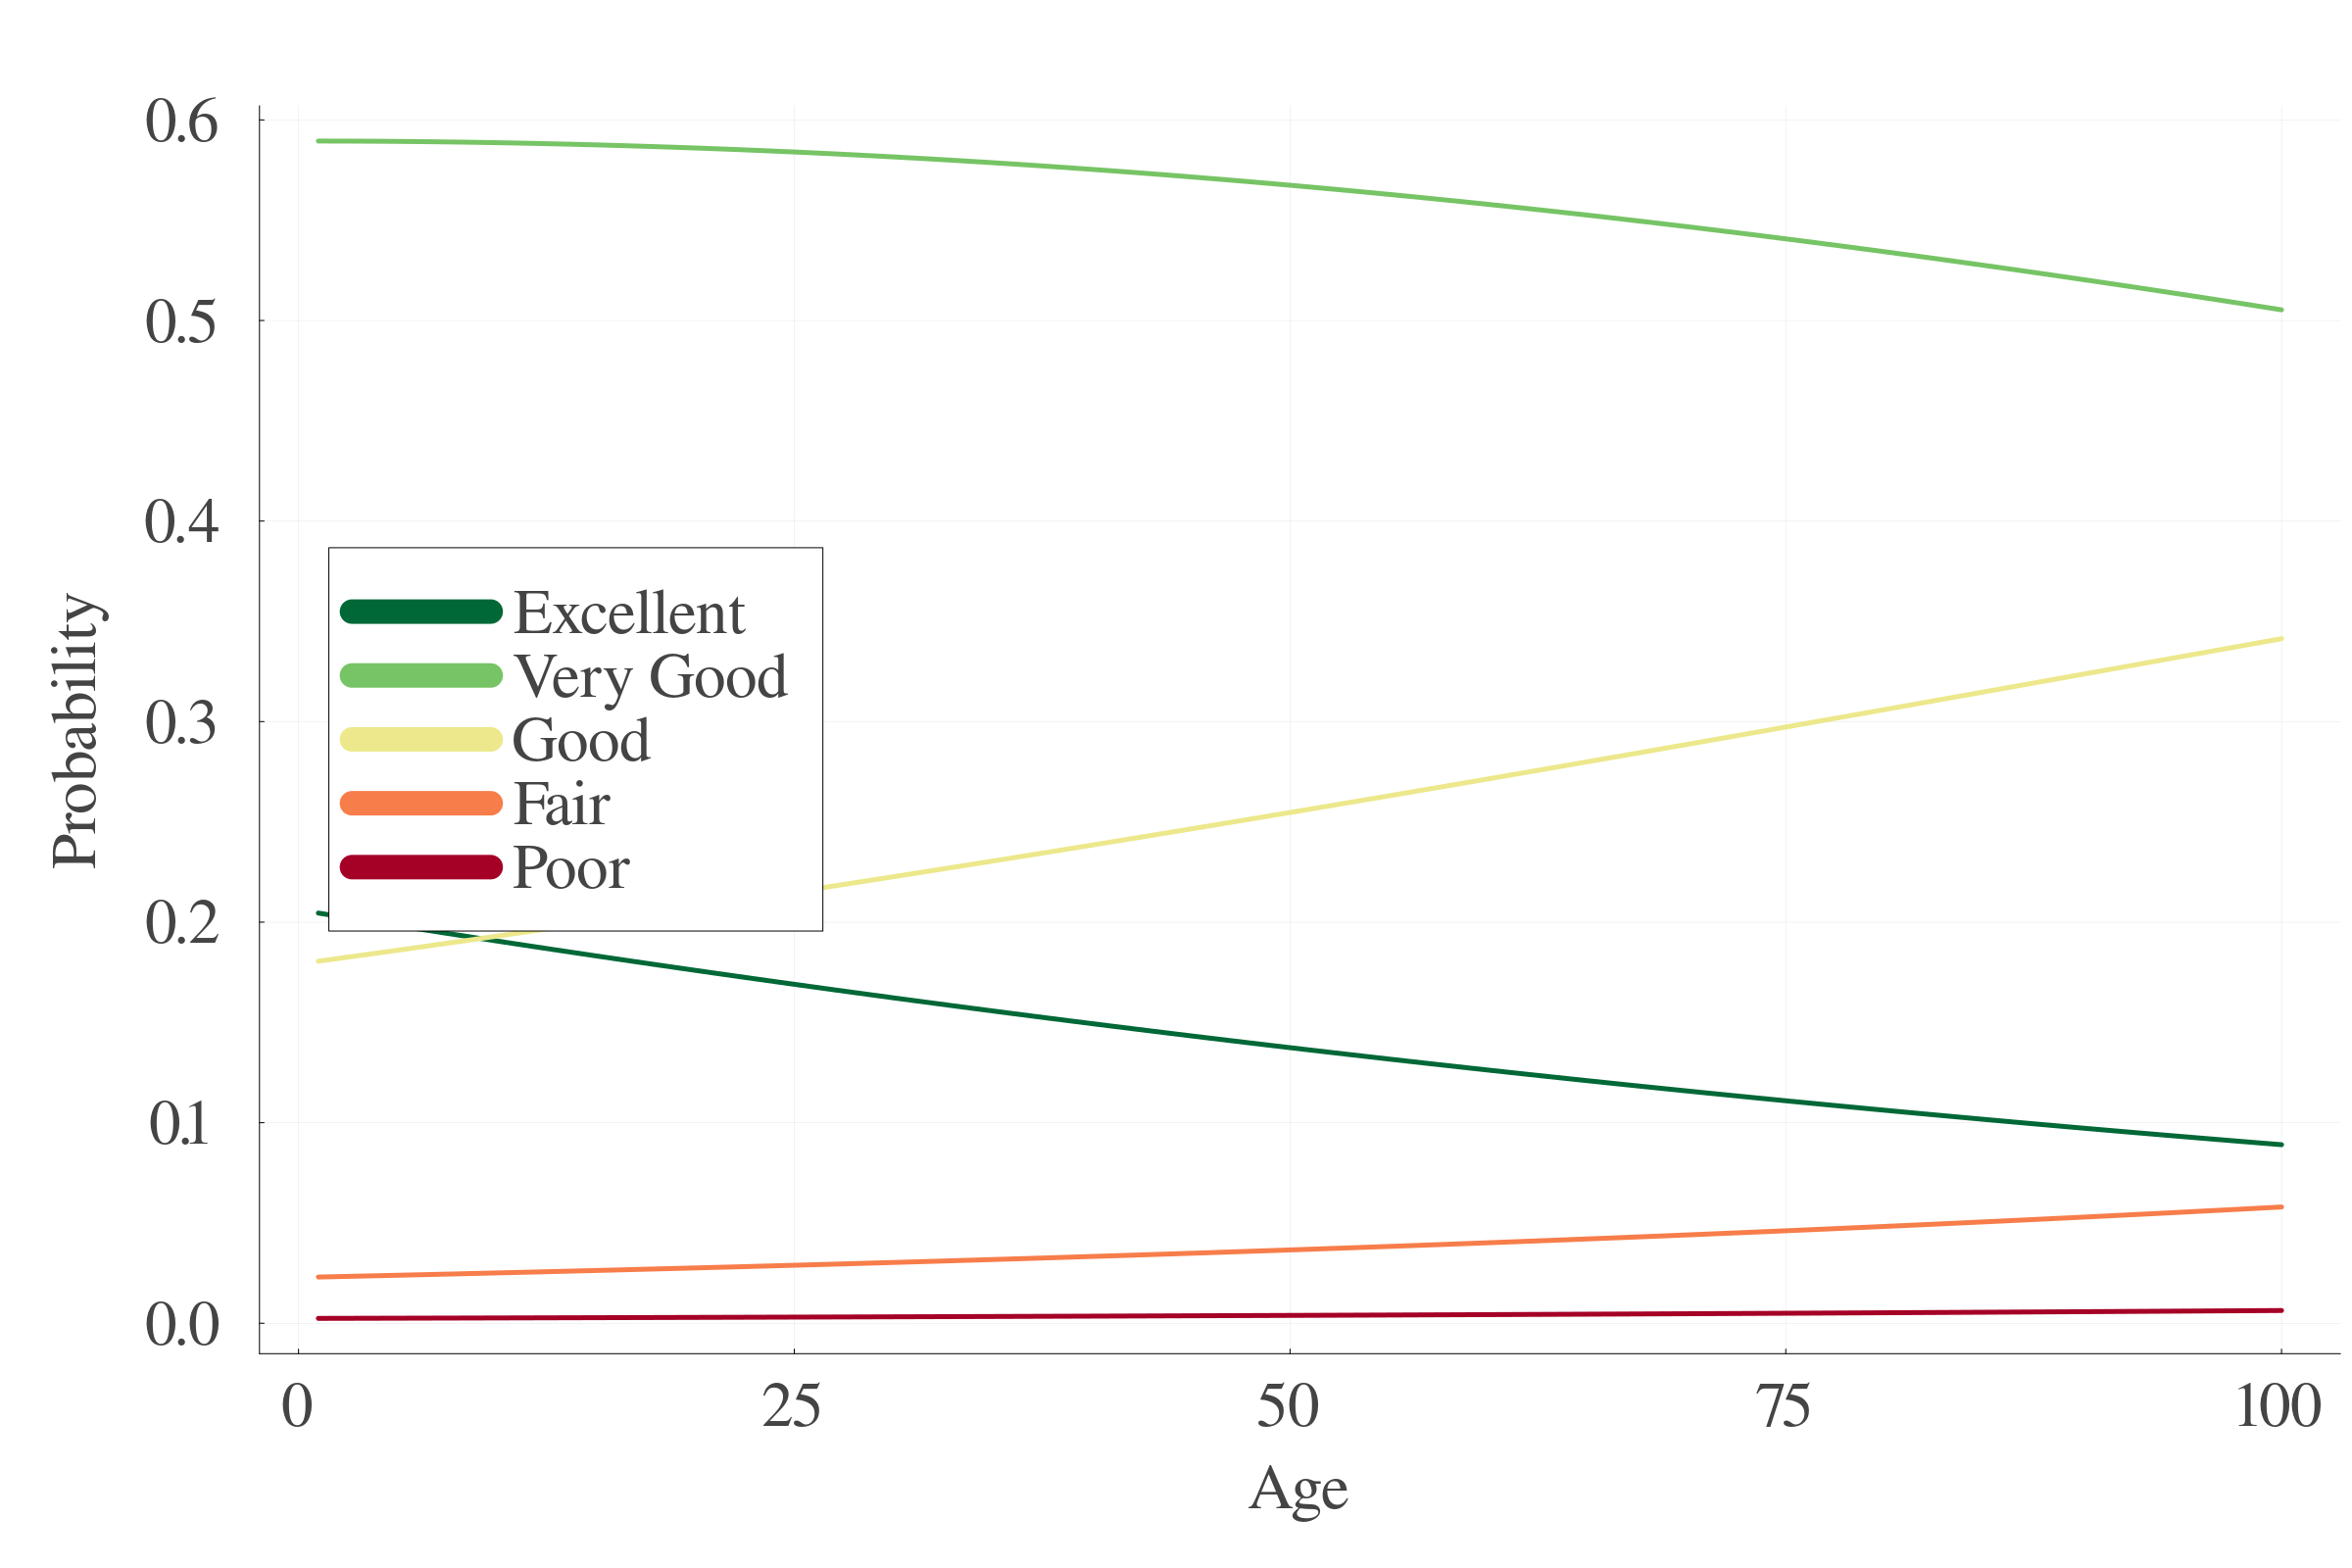
\includegraphics[width=0.4\linewidth]{output/health_transition_2.png}
        \caption{Transition probabilities from Very Good Health}    
    \end{center}
\end{figure}

\begin{figure}[H]\label{fig:health_transition_3}
    \begin{center}
        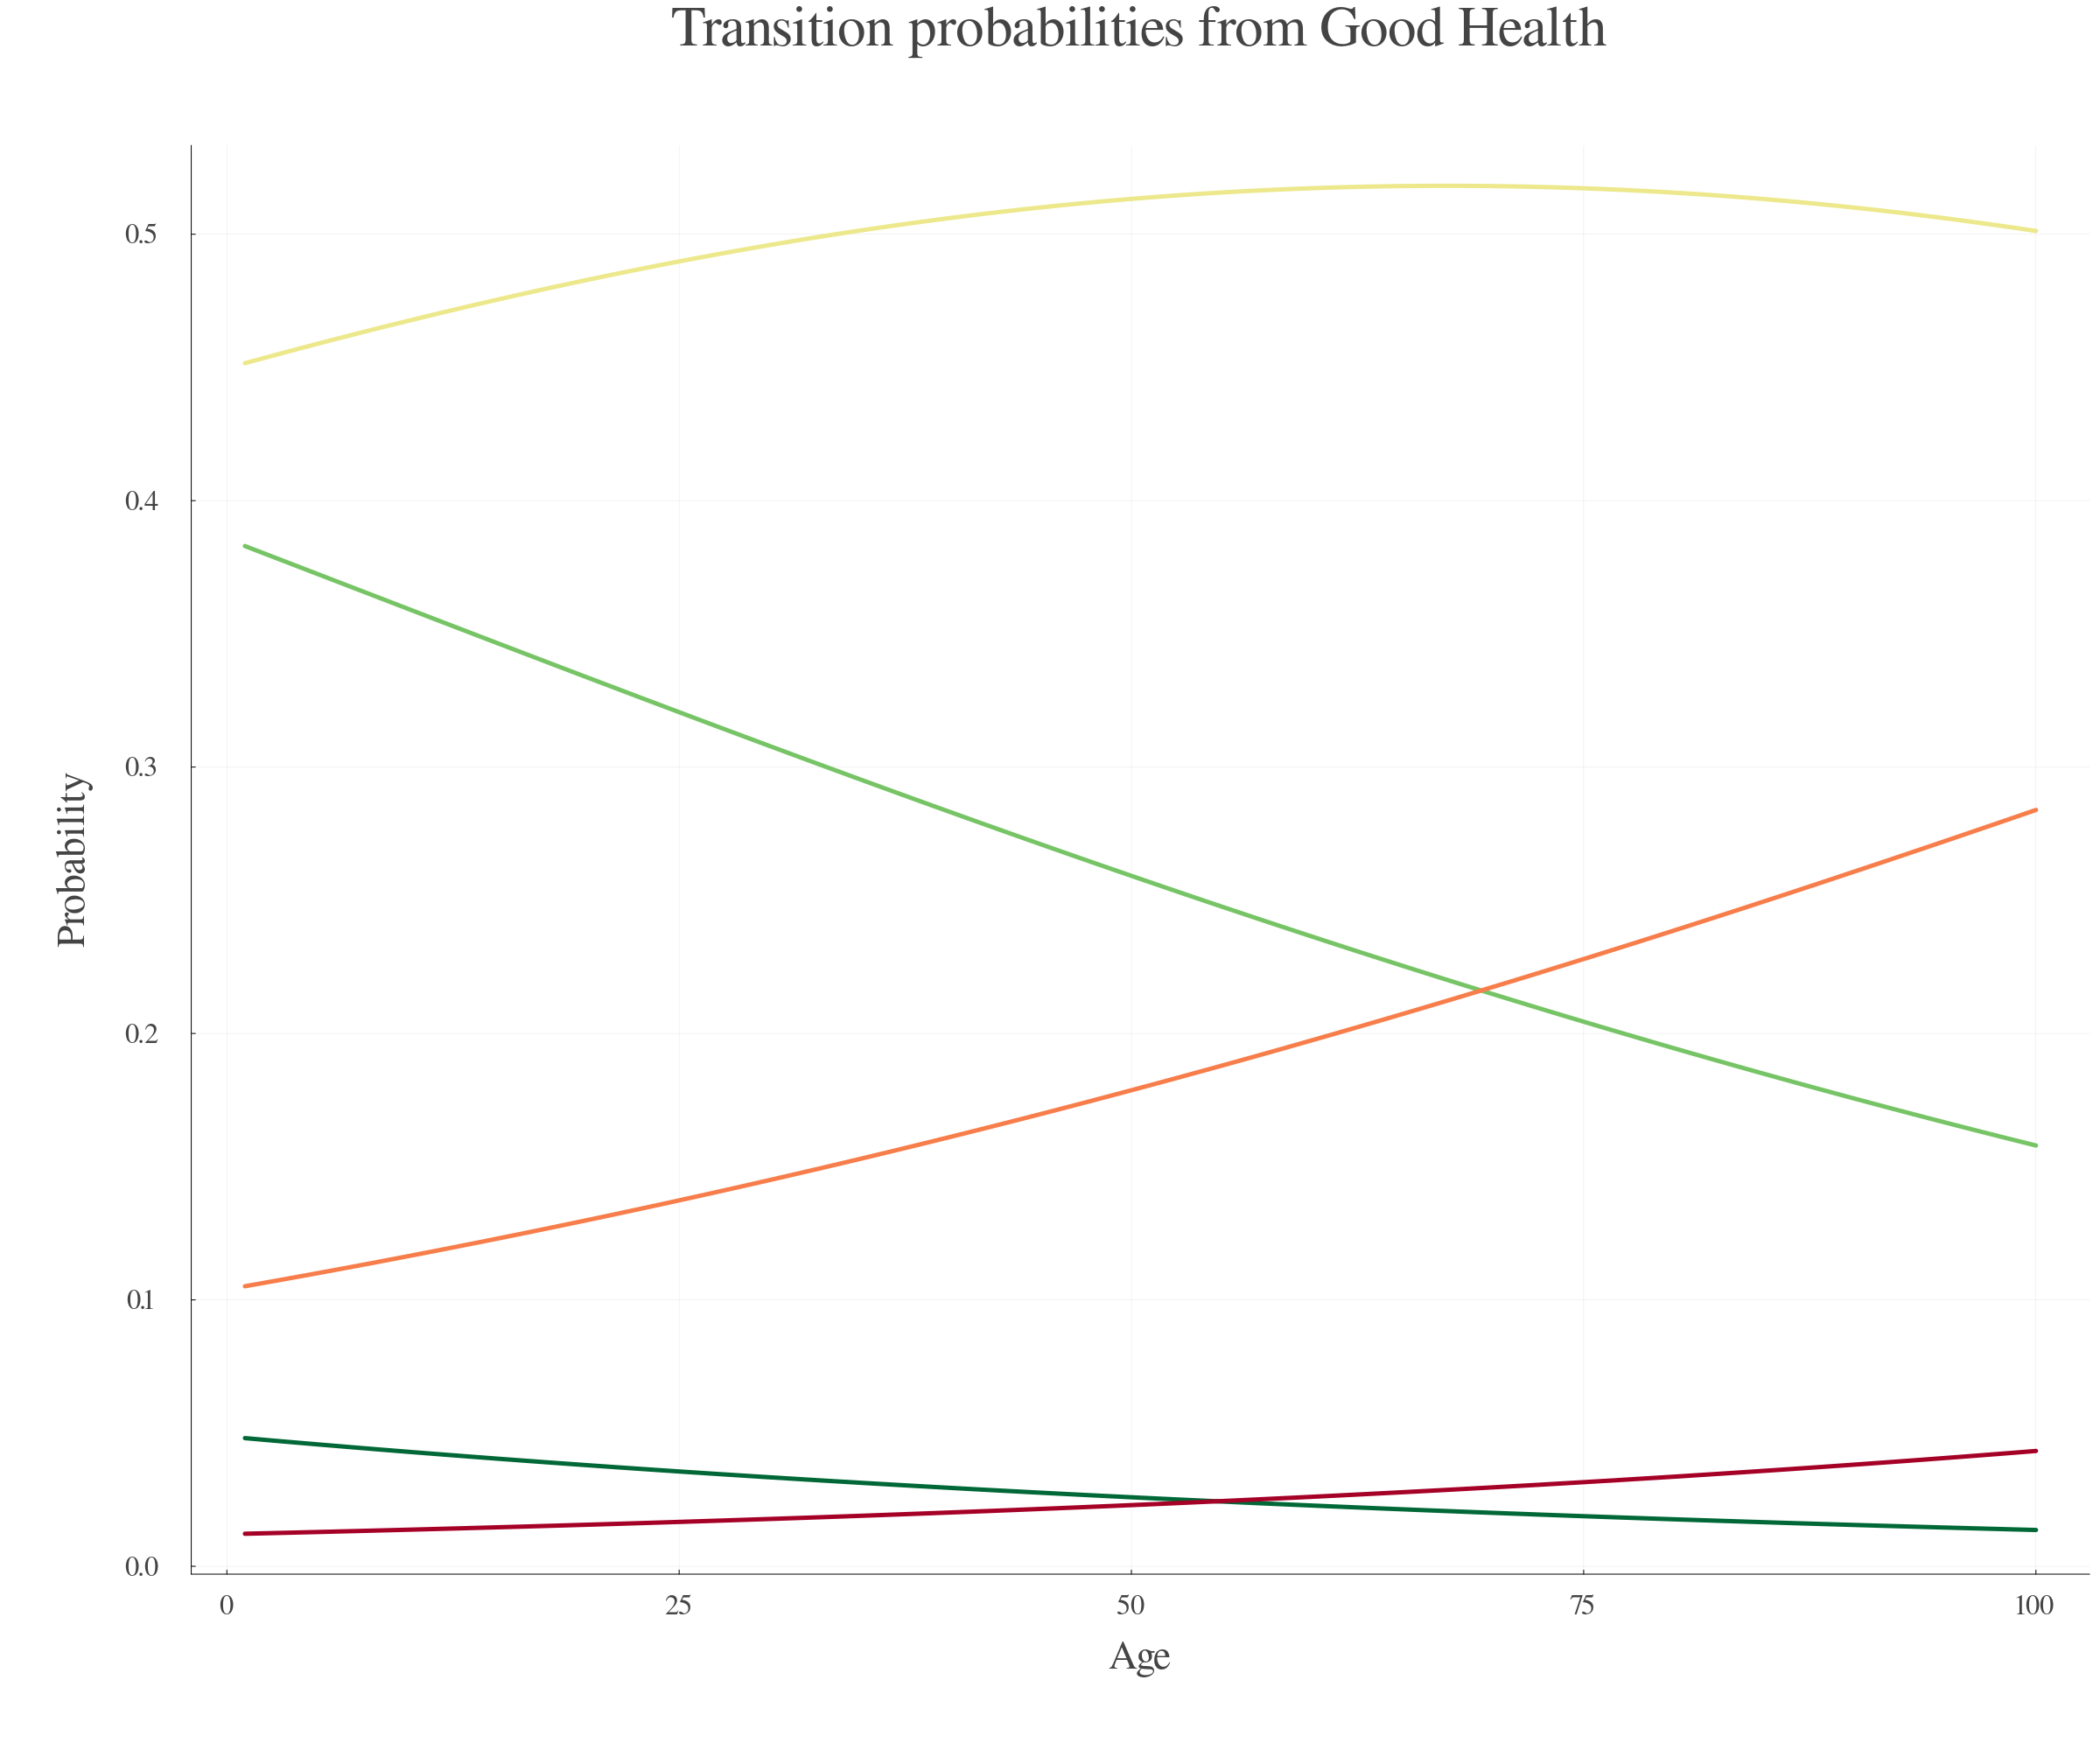
\includegraphics[width=0.4\linewidth]{output/health_transition_3.png}
        \caption{Transition probabilities from Good Health}  
    \end{center}  
\end{figure}

\begin{figure}[H]\label{fig:health_transition_4}
    \begin{center}
        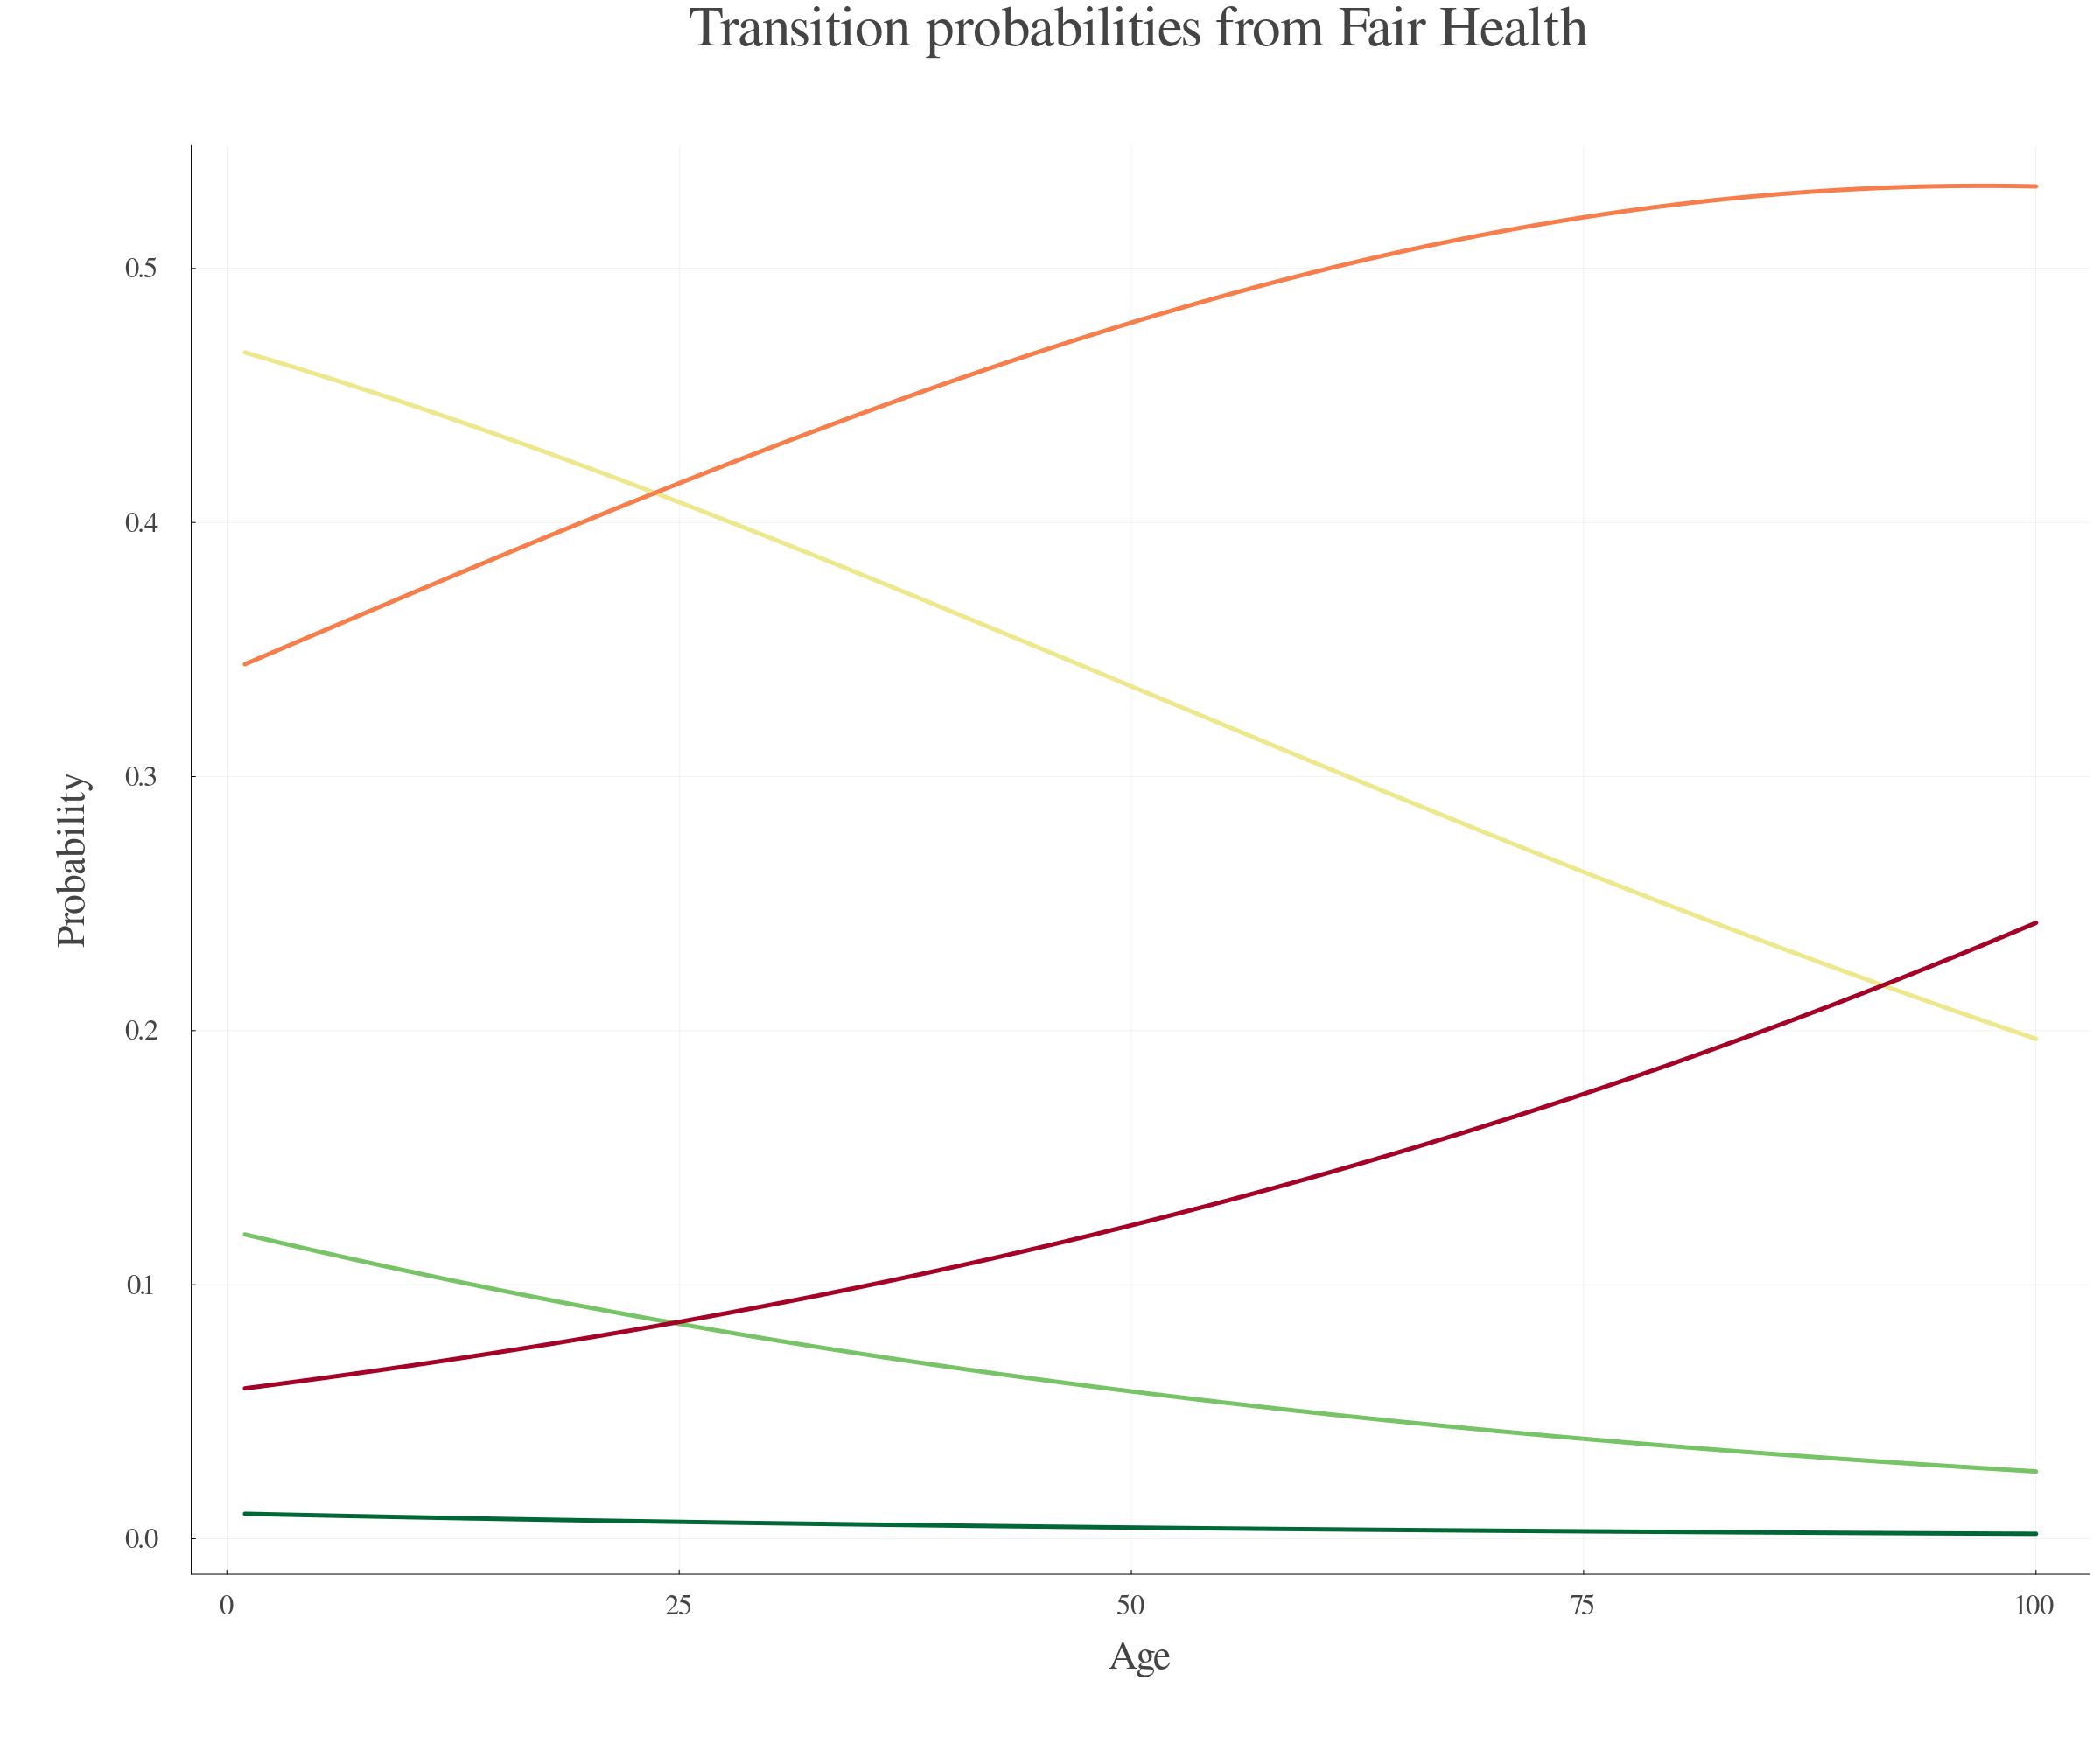
\includegraphics[width=0.4\linewidth]{output/health_transition_4.png}
        \caption{Transition probabilities from Fair Health}    
    \end{center}
\end{figure}

\subsection{Health simulation}

\begin{figure}[H]
    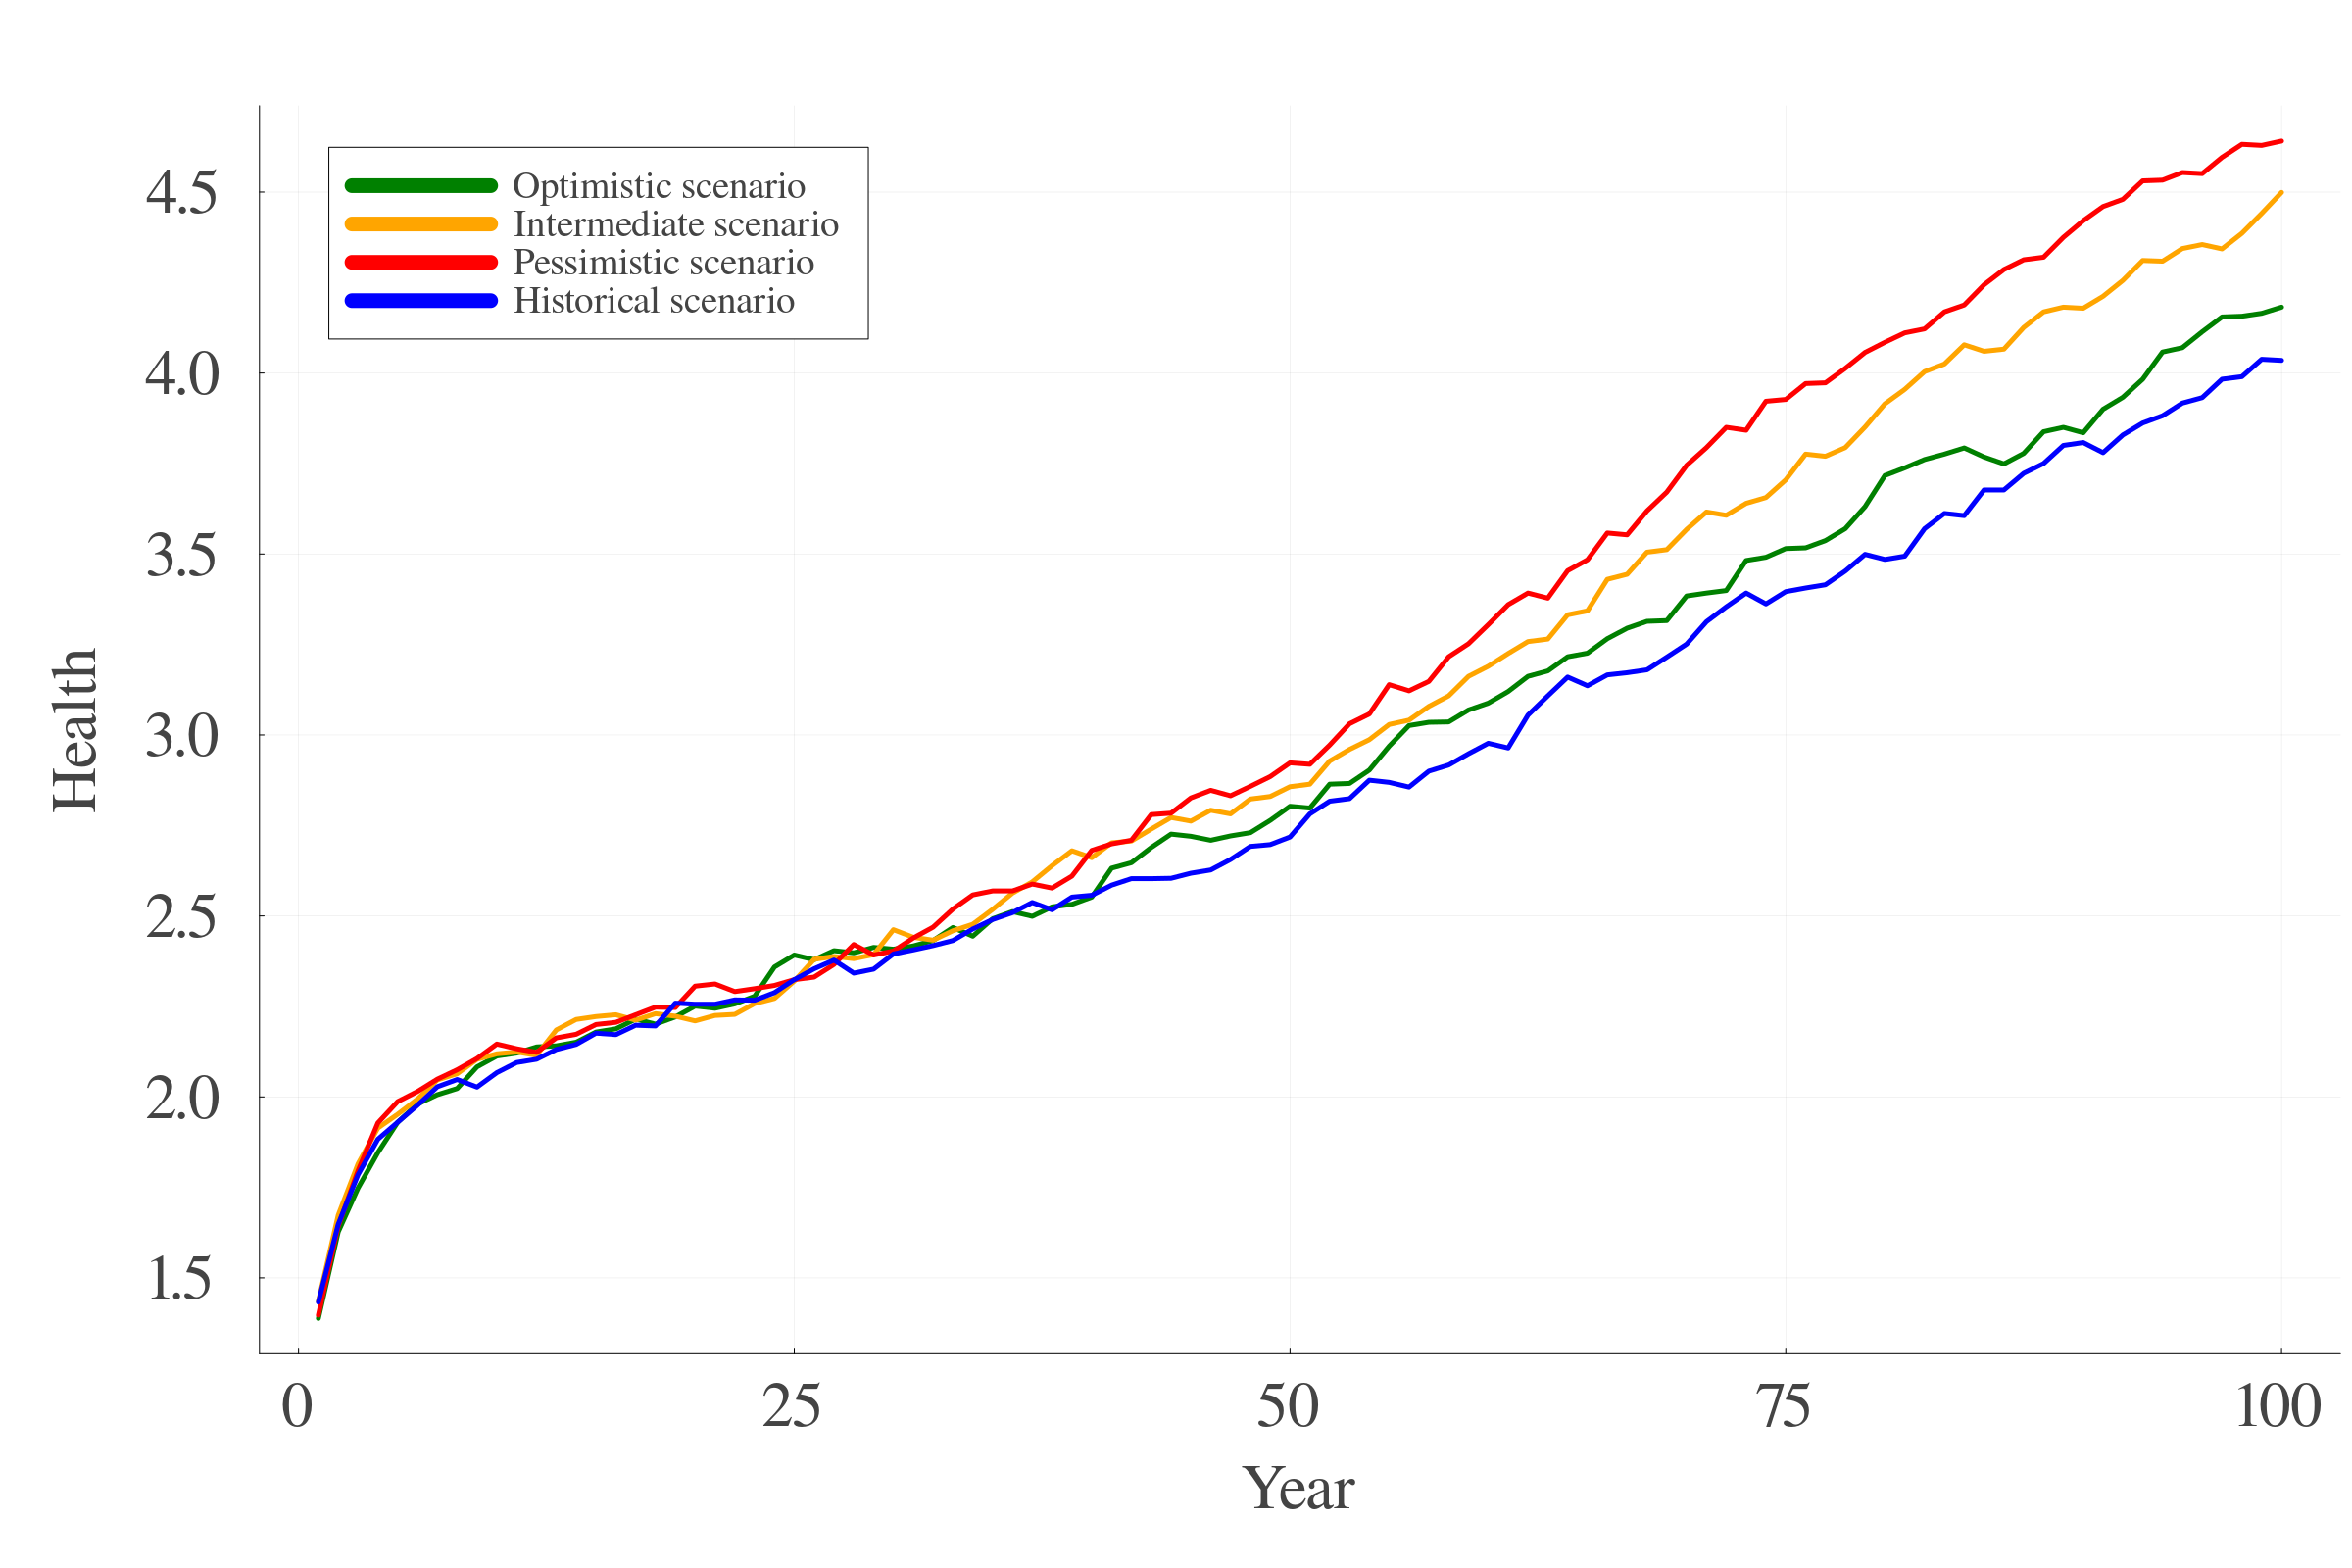
\includegraphics[width=\textwidth]{/Users/paulogcd/Documents/Master_Thesis/working_elements/Draft/output/average_health.png}
    \caption{Annual average health status as a function of temperature scenarios.}
\end{figure}

\subsection{Proof of Impossibility}

This section is dedicated to the proof that the maximization program
has no analytical solution in most cases.

Iwill show this absence of analytical solution by attempting to solve it in three different 
ways: First by using the Budget Constraint binding, then by using the F.O.C. and the Budget Constraint,
and lastly trying to go to the last period to solve it recursively. 

\subsubsection{Maximization program}

$$ \max_{\{c_{t},l_{t},s_{t+1}\}_{t=1}^{100}}
{\mathbb{E}\left[\sum_{t=1}^{100} \beta^{t}\cdot \frac{c_{t}^{1-\rho}}{1-\rho}-\xi_{t}\cdot \frac{l_{t}^{1+\varphi}}{1+\varphi}\right]}$$

Subject to budget and borrowing constraints:

$$c_{t} + s_{t+1} \leq l_{t}\cdot z_{t} + s_{t}\cdot(1+r_{t})$$

$$s_{t+1}\geq \underline{s}, \forall t \in [\![1,100]\!]$$

\subsubsection{Budget constraint binding}

A first solving attempt consists in assuming that the budget constraint binds.
We can then obtain the following expression for consumption: 

$$c_{t} = l_{t}\cdot z_{t} + s_{t}\cdot(1+r_{t}) - s_{t+1}$$

Plugging it into the maximization program, we obtain:

$$ \max_{\{l_{t},s_{t+1}\}_{t=1}^{100}}
{\mathbb{E}\left[\sum_{t=1}^{100} \beta^{t}\cdot \frac{\left(l_{t}\cdot z_{t} + s_{t}\cdot(1+r_{t}) - s_{t+1}\right)^{1-\rho}}{1-\rho}-\xi_{t}\cdot \frac{l_{t}^{1+\varphi}}{1+\varphi}\right]}$$

The F.O.C. with respect to labor implies: 

\begin{equation}
    l_{t}^{\varphi}\cdot \xi_{t} = \left[l_{t}\cdot z_{t} + s_{t}\cdot(1+r_{t})- s_{t+1}\right]^{-\rho}\cdot z_{t}
\end{equation}

We can develop the decomposition of consumption if and only if $\rho \in \mathbb{N}$.
Indeed, this equation is of form $x = (x-\alpha)^{\beta} \cdot z$.
With $\beta\notin \mathbb{N}$, is a transcendental equation.

\subsubsection{F.O.C. and Budget clearing}

We can now try to compute the F.O.C. first, and then make use of the Budget Constraint.
The Lagrangian function associated witht the maximization program of the agent is: 
\begin{equation}
    \begin{split}
        \mathcal{L}(c_{t},l_{t},s_{t+1};\lambda_t,\gamma_{t}) &
        = \mathbb{E}\Big[\sum_{t=1}^{100} \beta^{t}\cdot ((\frac{c_{t}^{1-\rho}}{1-\rho}-\xi_{t}\cdot\frac{l_{t}^{1+\varphi}}{1+\varphi}) \\
        & +\lambda_{t}\cdot \left(l_{t}\cdot z_{t}+s_{t}\cdot (1+r_{t})-c_{t}-s_{t+1}\right) \\ 
        & + \gamma_{t}\cdot \left(s_{t+1}-\underline{s}\right))\Big] \\ 
    \end{split}
\end{equation}

The First Order Conditions are the following:

$$\frac{\partial \mathcal{L}}{\partial c_{t}} = 0 \iff c_{t}^{-\rho} = \lambda_{t}$$


$$\frac{\partial \mathcal{L}}{\partial l_{t}} = 0 \iff \lambda_{t}\cdot z_{t} = \xi_{t}\cdot l_{t}^{\varphi}$$


$$\frac{\partial \mathcal{L}}{\partial s_{t+1}} = 0 \iff \lambda_{t} = \beta \cdot \mathbb{E}\left[\lambda_{t+1}\cdot (1+r_{t+1})\right] + \gamma_{t}$$

We first note that we must obtain a closed-form solution for $c_{t}$ and $l_{t}$ to obtain 
the optimal value of $s_{t+1}$. 
Indeed, since $s_{t+1}$ is linear in $\mathcal{L}$, we would need to plug the closed-form
solutions of $c_{t}$ and $l_{t}$ in the budget constraint. \\

Replacing the expression of $\lambda_{t}$ in the two other equation yields: 

\begin{equation}
    c^{-\rho}_{t}\cdot z_{t} = \xi_{t}\cdot l_{t}^{\varphi} \iff
        \begin{cases}
        & c_t = \left[\frac{\xi_{t}\cdot l_{t}^{\varphi}}{z_{t}}\right]^{-\frac{1}{\rho}}\\ 
        & l_{t} = \left[\frac{c_{t}^{-\rho}z_{t}\cdot}{\xi_{t}}\right]^{\frac{1}{\varphi}}
    \end{cases}
\end{equation}
And 
\begin{equation}
    c^{-\rho}_{t} = \beta \cdot \mathbb{E}\left[c^{-\rho}_{t+1}\cdot (1+r_{t+1})\right] + \gamma_{t}
\end{equation}

Assuming that the budget constraint binds, it becomes, as previously seen:

$$c_{t} + s_{t+1} = l_{t}\cdot z_{t} + s_{t}\cdot(1+r_{t})
\iff 
c_{t} = l_{t}\cdot z_{t} + s_{t}\cdot(1+r_{t}) - s_{t+1} 
$$

This leads to the following equation system: 

$$
\begin{cases}
    & c_t = \left[\frac{\xi_{t}\cdot l_{t}^{\varphi}}{z_{t}}\right]^{-\frac{1}{\rho}} \\
    & c_{t} = l_{t}\cdot z_{t} + s_{t}\cdot(1+r_{t}) - s_{t+1} 
\end{cases}
$$

$$\iff$$
$$ \left[\frac{\xi_{t}\cdot l_{t}^{\varphi}}{z_{t}}\right]^{-\frac{1}{\rho}} = l_{t}\cdot z_{t} + s_{t}\cdot(1+r_{t}) - s_{t+1} $$
$$\iff$$
$$ l_{t}^{-\frac{\varphi}{\rho}} \cdot \left(\frac{\xi_{t}}{z_{t}}\right)^{-\frac{1}{\rho}} = l_{t}\cdot z_{t} + s_{t}\cdot(1+r_{t}) - s_{t+1} $$
$$\iff$$
$$ l_{t}^{-\frac{\varphi}{\rho}} \cdot \left(\frac{z_{t}}{\xi_{t}}\right)^{\frac{1}{\rho}} - l_{t}\cdot z_{t} - s_{t}\cdot(1+r_{t}) - s_{t+1} = 0 $$

This is a transcendental equation of form 
$x^{\alpha}\cdot b - x\cdot y - c = 0$,
which admits a solution if and only if $-\frac{\varphi}{\rho} \in \mathbb{N}$.
This condition seems unrealistic in our context: 

\begin{itemize}
    \item $-\varphi >0$ implies that labor has a decreasing disutility,
    which makes the maximization program absurd.
    \item $-\rho >0$ implies a risk-loving agent, which changes 
    drastically the framework of our model, and would require another whole 
    interpretation.
\end{itemize}

Note that if we set $-\rho\in\mathbb{N}$ and further develop the last equation in the 
budget constraint binding attempt, we end up with the same condition.

\subsubsection{Backwards solving attempt}

If we try to solve it backwards, we now go to the last period. 
At the last period, $s_{t+1} = \underline{s}$ for sure:
Since there is no future, 
the agent will borrow as much as they can,
or will at least not save anything more than what is imposed 
by the constraint. 

For simplification, let $\underline{s}$ be fixed such that: $\underline{s} = 0$.
The new optimality condition is: 

\begin{equation}
    l_{t}^{\varphi}\cdot \xi_{t} = \left[l_{t}\cdot z_{t} + s_{t}\cdot(1+r_{t})\right]^{-\rho}\cdot z_{t}
\end{equation}

Although we simplified the term at the exponential of which 
we have $-\rho$, this is still a transcendental equation due to the sum 
of labor income and income coming from savings of last period, 
and the problem remain the same.

\end{document}